%instiki:category: FisicaSubatomica
\chapter{Principio Gauge Local}
\label{cha:princ-gauge-local} %noinstiki
%instiki:
%instiki:***
%instiki:
%instiki:[[NotasFS|Tabla de Contenidos]]
%instiki:
%instiki:***
%instiki:
%instiki:* [Ecuaci\'on de klein-Gordon](#ecuacion-de-klein)
%instiki:
%instiki:* [Campos escalares complejos](#camp-escal-compl)
%instiki:
%instiki:* [Invarianza gauge local abeliana](#invar-gauge-local)
%instiki:
%instiki:* [Aplicaci\'on a la mec\'anica cu\'antica](#aplic-la-mecan)
%instiki:
%instiki:* [Invarianza gauge local no abeliana](#invar-gauge-local-2)
%instiki:
%instiki:* [Invarianza gauge local para un grupo semisimple](#invar-gauge-local-1)
%instiki:
%instiki:* [$\Phi$ como un triplete de $SU(2)$](#phi-como-un)
%instiki:
%instiki:* [Problemas](#problemas-3)
%instiki:
%instiki:***
%instiki:


\section{Electrodinámica Cuántica}
\label{sec:electr-cuant}

Para hacer el Lagrangiano en ec.~\eqref{eq:115qft} invariante gauge local bajo $U(1)_Q$, procedemos de la forma usual. El campo transforma como
\begin{align}
  \psi\to\psi'=e^{-i\theta(x)Q}\psi\nonumber\\
  \bar{\psi}\to\bar{\psi}'=\bar{\psi}e^{i\theta(x)Q}\,,
\end{align}
donde $Q$ es el generador de carga eléctrica en unidades de la carga del electrón.

La derivada covariante se define de manera que transforma de la misma forma que el campo, introduciendo el campo gauge $A^\mu$
\begin{equation}
  \label{eq:202qft}
  \partial^\mu\to\mathcal{D}^\mu=\partial^\mu-ieQA^\mu\,,
\end{equation}
donde $e$ es la carga eléctrica del electrón. De esta forma, si $\psi_e$ es el campo que representa al electrón
\begin{align}
  eQ \psi_e=e(-1)\psi_e=-e \psi_e\,.
\end{align}

El Lagrangiano correspondiente a la interacción de un fermión y el campo electromagnético corresponde al Lagrangiano de Dirac con la derivada normal reemplzada por la derivada covariante, y el correspondiente término cinético invariante gauge y de Lorentz asociado al nuevo campo introducido en la derivada covariante: $A^\mu$. Este campo es necesario para compensar los cambios en la energía y momentum que sufre el electrón como consecuencia de imponer la invarianza de la Acción bajo un cambio de fase local 
\begin{equation}
  \label{eq:201qft}
  \mathcal{L}=\overline{\psi}\left(i\gamma^\mu\mathcal{D}_\mu-m\right)\psi -\tfrac{1}{4}F^{\mu\nu}F_{\mu\nu},
\end{equation}
y es invariante bajo transformaciones locales $U(1)_Q$. Desarrollando la expresión anterior, tenemos
\begin{align}
    \mathcal{L}&=\bar{\psi}\left[i\gamma^\mu\left(\partial_\mu-ieQA_\mu\right)-m\right]\psi -\tfrac{1}{4}F^{\mu\nu}F_{\mu\nu}\nonumber\\
    &=\bar{\psi}\left(i\gamma^\mu\partial_\mu-m\right)\psi+eQ\bar{\psi}\gamma^\mu\psi A_\mu -\tfrac{1}{4}F^{\mu\nu}F_{\mu\nu}.
\end{align}
Este Lagrangiano da lugar a la Acción de la teoría conocida como Electrodinámica Cuántica (QED de sus siglas en inglés).

Aplicando las ecuaciones de Euler-Lagrange para $\bar{\psi}$, tenemos
\begin{align}
  (i\gamma^\mu\partial_\mu-m)\psi+eQ\gamma^\mu A_\mu\psi=0\nonumber\\
  (i\gamma^\mu\partial_\mu-i^2eQ\gamma^\mu A_\mu-m)\psi=0\nonumber\\
  [i\gamma^\mu(\partial_\mu-ieQA_\mu)-m]\psi=0\nonumber\\
  (i\gamma^\mu\mathcal{D}_\mu-m)\psi=0.
\end{align}
Que corresponde a la ecuación de Dirac en presencia del campo electromagnético. Mientras que para el campo $A^\mu$, tenemos
\begin{align}
  -\frac{1}{4}\partial_\mu\left[\frac{F^{\rho\eta}F_{\rho\eta}}{\partial\left(\partial_\mu A_\nu\right)}\right]-eQ\bar{\psi}\gamma^\rho\psi\frac{\partial A_\rho}{\partial A_\nu}&=0\nonumber\\
  \partial_\mu F^{\mu\nu}&=-eQ\bar{\psi}\gamma^\nu\psi
\end{align}
Definimos entonces la corriente electromagnética generada por el fermión como
\begin{equation}
  \label{eq:222qft}
  j^\mu=-eQ\bar{\psi}\gamma^\mu\psi.
\end{equation}
De nuevo, la aparición de la interacción electromagnética es una consecuencia de la invarianza gauge local. 

El cálculo directo de la  corriente 
\begin{align}
  J^\mu&=\frac{\partial\mathcal{L}}{\partial\left(\partial_\mu\psi\right)}\delta\psi+\delta\bar{\psi}\frac{\partial\mathcal{L}}{\partial\left(\partial_\mu\bar{\psi}\right)}\nonumber\\
  &= i\overline{\psi}\gamma^\mu(-i \theta(x) Q ) \psi
  &= \theta(x) Q\overline{\psi}\gamma^\mu \psi\,,
\end{align}
y para la ecuación de Dirac, a diferencia de la ecuación de Schrödinger, la corriente de probabilidad tiene la misma forma que la corriente electromagnética.

De esta manera podemos reescribir el Lagrangiano en términos de un Lagrangiano libre y otro de interacción
\begin{align}
  \mathcal{L}=\mathcal{L}_{\text{free}}+\mathcal{L}_{\text{int}}\,,
\end{align}
\begin{align}
  \mathcal{L}_{free}=&\bar{\psi}\left(i\gamma^\mu\partial_\mu-m\right)\psi-\tfrac{1}{4}F^{\mu\nu}F_{\mu\nu}\nonumber\\
  \mathcal{L}_{\text{int}}=&eQ\bar{\psi}\gamma^\mu\psi A_\mu\,.
\end{align}
Para la QED sólo hay un término de interacción que es suficiente para explicar todos los fenoménos electromagnéticos y su interacción con la materia. Este esta representado por el diagrama de Feynman mostrado en la Figura \ref{fig:feynmanruleqed}

\begin{figure}
  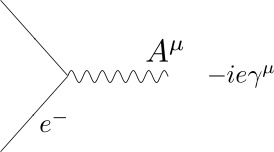
\includegraphics{feynmanruleqed} % in feynmanrules.svf as a Layer
  \caption{Feynman rule for QED}
  \label{fig:feynmanruleqed}
\end{figure}

La repulsión electromagnética esta representada por la figura \ref{fig:qedrepulsion}. En la Figura (a) el primer electrón emite un fotón y se dispersa, mientras que el segundo absorbe el fotón y se dispersa en la dirección opuesta. En la Figura (b) el primer electón absorve el fotón emitido por el segundo electrón. Los dos diagrams se representa por uno único con el fotón en horizontal como se muestra en la Figura (c).

\begin{figure}
  \centering
  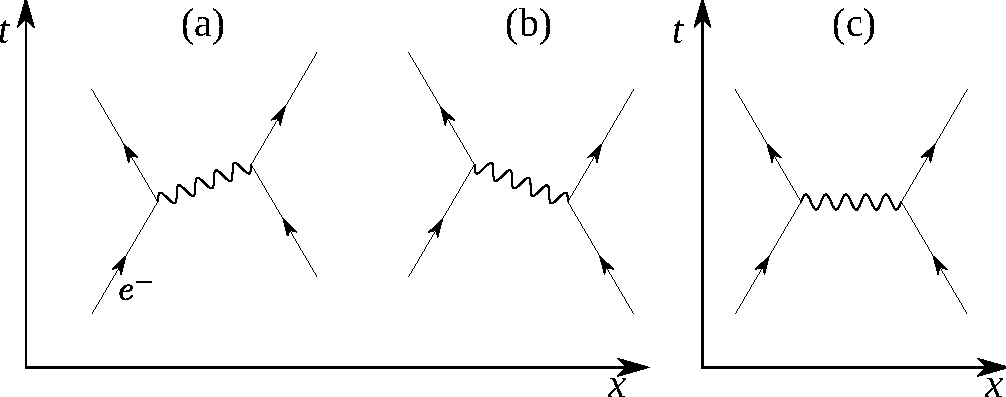
\includegraphics{qedrepulsion}
  \caption{Electromagnetic repulsion. The diagrams (a) and (b) are summarized in the diagram (c)}
  \label{fig:qedrepulsion}
\end{figure}


%Intentando obtener el operador Hamiltoniano y demás:
%  \begin{align}
%   T^\mu_\nu=&\frac{\partial\mathcal{L}}{\partial\left(\partial_\mu\psi\right)}\partial_\nu\psi+\partial_\nu\bar{\psi}\frac{\partial\mathcal{L}}{\partial\left(\partial_\mu\bar{\psi}\right)}-\mathcal{L}\delta^\mu_\nu\nonumber\\
%   =&i\bar{\psi}\gamma^\mu\partial_\nu\psi-\mathcal{L}\delta^\mu_\nu\,.
% \end{align}
% La expresión para $T^0_i$ es la misma que antes
% \begin{align}
%   T^0_0=i\psi^\dagger\partial_0\psi-i\psi^\dagger\partial_0\psi-i\psi^\dagger\gamma^0\gamma^i\partial_i\psi+m\psi^\dagger\psi-eQ\bar{\psi}\gamma^\mu\psi A_\mu +\tfrac{1}{4}F^{\mu\nu}F_{\mu\nu}.
% \end{align}



\section{Cromodinámica Cuántica}
\label{sec:inter-fuert}
Los protones, neutrones, piones, kaones y demás hadrones, son partículas compuestas de constituyentes elementales llamados quarks. Por ejemplo los protones, neutrones y piones están constituidos de quarks up y down. Los hadrones están dividos en  bariones, $B$, constituidos de tres quarks, y los mesones, $M$, de dos. Para satisfacer el principio de exclusión de Pauli, y justificar el confinamiento de los hadrones, se requiere que cada quark contenga $N_c$ cargas diferentes, llamadas cargas de color, de manera que la carga de color de un hadrón sea cero. Muchos resultados experimentales respaldan la existencia de tres cargas de color para cada quark, $N_c=3$. De este modo cada quark $q=u,d,c,s,t,b$ viene en tres colores
\begin{equation}
  q_\alpha=q_1,q_2,q_3=q_r,q_b,q_g,
\end{equation}
donde los últimos subíndices hacen referencia a los colores red, blue, green. De este modo los Bariones y mesones están descritos por combinaciones singletes de color del tipo $q_r q_b q_g$ y $q_r\bar{q}_r$,
\begin{equation}
\label{eq:199qft}
  B=\frac{1}{\sqrt{6}}\epsilon_{\alpha\beta\gamma}
  \left|q_\alpha q_\beta q_\gamma\right\rangle \qquad M=\frac{1}{\sqrt{3}}\delta^{\alpha\beta}\left|\bar{q}_{\alpha}q_\beta\right\rangle
\end{equation}
Estos estados son singletes de color.
Una de las determinaciones de $N_c$ proviene del observable
\begin{align}
  R\approx&\frac{\sigma(e^+e^-\to\text{hadrones})}{\sigma(e^+e^-\to\mu^+\mu^-)}
\end{align}

Para $f=u,d,s,c,b,t$, (en orden de masa) tenemos que para una energía donde se pueden producir hadrones compuestos de hasta  quarks $f_{\text{max}}$
\begin{align}
  R\approx&\frac{\sum_{f=u}^{f_{\text{max}}}\sum_{\alpha=1}^{N_c}\sigma(e^+e^-\to f_\alpha\bar{f}_\alpha)}{\sigma(e^+e^-\to\mu^+\mu^-)}\nonumber\\
  R\approx&N_c\frac{\sum_{f=u}^{f_{\text{max}}}\sigma(e^+e^-\to f\bar{f})}{\sigma(e^+e^-\to\mu^+\mu^-)}
\end{align}
De este modo $R$ esta dado por la suma de las cargas eléctricas al cuadrado
\begin{align}
\label{eq:254qft}
R\approx&N_c\frac{\sum_f Q_f^2}{Q_\mu^2}\nonumber\\
=&N_c\sum_{f=u}^{f_{\text{max}}} Q_f^2\nonumber\\
=&
\begin{cases}
  N_c[(\frac{2}{3})^2+2(\frac{-1}{3})^2]=\frac{2}{3}N_c&f=u,d,s,\;f_{\text{max}}=s\\
  N_c[2(\frac{2}{3})^2+2(\frac{-1}{3})^2]=\frac{10}{9}N_c&f_{\text{max}}=c\\
  N_c[2(\frac{2}{3})^2+3(\frac{-1}{3})^2]=\frac{11}{9}N_c&f_{\text{max}}=b
\end{cases}\nonumber\\
=&
\begin{cases}
  2&N_c=3,\qquad f_{\text{max}}=s\\
  \frac{10}{3}&N_c=3,\qquad f_{\text{max}}=c\\
  \frac{11}{3}&N_c=3,\qquad f_{\text{max}}=b\\
\end{cases}
\end{align}
%\left(\right)
En la figura, tomada de \cite{a}, se muestra el gráfico de $R$ con respecto a $\sqrt{s}$ (la energía de centro de masa de la colisión). Se observan dos escalones, uno que va hasta una energía $\sqrt{s}\approx4\,$GeV que corresponden a $f=u,d,s$, con un $R\approx2$,  y otro hasta $\sqrt{s}\approx40\,$GeV que corresponde a $f=u,d,s,c,b$, con un $R\approx3.7\approx11/3$. Los dos valores de $R$ son compatibles con los esperados de la ec.~\eqref{eq:254qft}. Como referencia también se señalan los valores para $N_c=4$ (en rojo). 
\begin{figure}
  \centering
  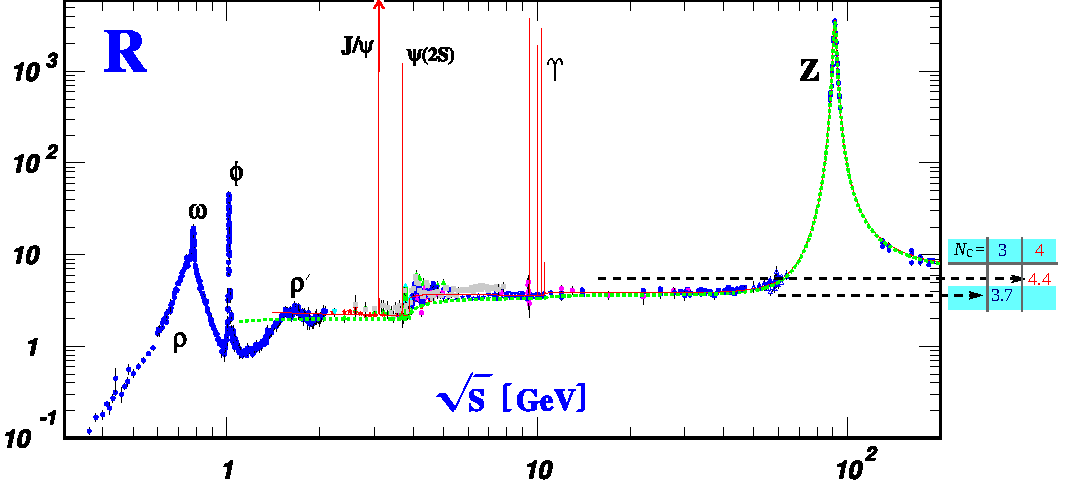
\includegraphics[scale=0.9]{r}
  \caption{Datos para $R$}
  \label{fig:r}
\end{figure}

Si queremos que el color sea una carga conservada como la carga eléctrica, ésta debe ser la consecuencia de una simetría gauge local. Para tener tres cargas diferentes la posibilidad más simple es imponer la simetría $SU(3)_c$, tal que tengamos un vector compuesto de 3 espinores de Dirac en el espacio de color:
\begin{equation}
  \Psi=
  \begin{pmatrix}
    \psi_r\\
    \psi_b\\
    \psi_g
  \end{pmatrix}
  =
  \begin{pmatrix}
    q_r\\
    q_b\\
    q_g
  \end{pmatrix}.
\end{equation}
El Lagrangiano de Dirac con invarianza gauge global $SU(3)$, para un quark, se puede escribir como
\begin{equation}
  \label{eq:128qft}
  \mathcal{L}_{\text{global}}=i\bar{\Psi}\gamma^\mu\partial_\mu\Psi-m\bar{\Psi}\Psi,
\end{equation}
donde
\begin{equation}
  \Psi\to \Psi'=\exp\left(i\theta_a\frac{\lambda^a}{2}\right)\Psi.
\end{equation}
$a=1,\ldots,8$, $\lambda_a/2$ son los ocho generadores de $SU(3)$ y $\theta_a$ son los parámetros de la transformación global. Los generadores de $SU(3)$
\begin{align}
  \Lambda^a\equiv\frac{\lambda^a}{2}\,,
\end{align}
satisfacen el álgebra
\begin{equation}
  \left[\frac{\lambda^a}{2},\frac{\lambda^b}{2}\right]=if^{abc}\frac{\lambda^c}{2}\,,
\end{equation}
donde $f^{abc}$ son las constantes de estructura fina de $SU(3)$.

En un análisis similar al de la sección \ref{sec:diracs-lagrangian} tenemos que la Acción invariante gauge local bajo $SU(3)_c$, se obtiene de reemplazar la derivada normal por la derivada covariante 
\begin{equation}
  \label{eq:127qft}
  \mathcal{L}_{\text{local}}=i\bar{\Psi}\gamma^\mu\mathcal{D}_\mu\Psi-m\bar{\Psi}\Psi
  -\frac{1}{2}\operatorname{Tr}\left({G}^{\mu\nu}{G}_{\mu\nu}\right),
\end{equation}
donde
\begin{align}
  \label{eq:qcdtr}
  \Psi\to \Psi'&=U(x)\Psi\nonumber\\
  \mathcal{D}_\mu\Psi\to \left(\mathcal{D}_\mu\Psi\right)'&
  =U(x)\mathcal{D}_\mu\Psi,
\end{align}
con la matriz $3\times 3$
\begin{align}
  U(x)=\exp\left[i\theta_a(x)\frac{\lambda^a}{2}\right]\,,
\end{align}
y
\begin{equation}
  \mathcal{D}_\mu=\partial_\mu-i g_s\frac{\lambda_a}{2}G_\mu^a\equiv\partial_\mu-i g_s {G}_\mu
\end{equation}
donde hemos definido la matriz $3\times 3$  $G_\mu$, como
\begin{equation}
  \left({G}_\mu\right)_{\alpha\beta}=\left(\frac{\lambda_a}{2}\right)_{\alpha\beta}G_\mu^a
\end{equation}

Este Lagrangiano da lugar a la interacción fuerte y es llamado el Lagrangiano de la Cromodinámica Cuántica, o el Lagrangiano de la QCD de sus siglas en Inglés.

De \eqref{eq:qcdtr}, tenemos
\begin{align}
   \mathcal{D}_\mu\Psi\to \left(\mathcal{D}_\mu\Psi\right)'=&\mathcal{D}'_\mu\Psi'
  =U(x)\mathcal{D}_\mu\Psi\nonumber\\
\mathcal{D}'_\mu U\Psi
  =U(x)\mathcal{D}_\mu\Psi\,.
\end{align}
Por consiguiente
\begin{equation}
  {\mathcal{D}'}^\mu U=U\mathcal{D}^\mu
\end{equation}
\begin{equation}
  \mathcal{D}^\mu\to\left(
    \mathcal{D}^\mu
  \right)'=U\mathcal{D}^\mu U^{-1}
\end{equation}
Desarrollando a ambos lados
\begin{align}
  \label{eq:251qft}
   {\mathcal{D}}^\mu\psi\to{\left({\mathcal{D}}^\mu\psi\right)}'=
  {\mathcal{D}^\mu}'\psi'=&{\mathcal{D}^\mu}'\psi'\nonumber\\
  (\partial^\mu-i g_s {G'}^\mu) U\psi=&U\mathcal{D}^\mu U^{-1}U\psi\nonumber\\
  (\partial^\mu-i g_s {G'}^\mu) U\psi=&U(\partial^\mu-i g_s {G}^\mu)\psi\nonumber\\
  U\partial^\mu\psi+(\partial^\mu U)\psi-i g_s {G'}^\mu U \psi=&U\partial^\mu\phi-i g_s U {G}^\mu \psi\nonumber\\
  (\partial^\mu U)\psi-i g_s {G'}^\mu U \psi=&-i g_s U {G}^\mu \psi\nonumber\\
  -i g_s {G'}^\mu U \psi=&-(\partial^\mu U)\psi-i g_s U {G}^\mu \psi\,,
\end{align}
de modo que
\begin{align}
     {G'}^\mu U =&\frac{1}{i g_s}(\partial^\mu U)+ U{G}^\mu \nonumber\\
   {G'}^\mu  =&-\frac{i}{g_s}(\partial^\mu U)U^{-1}+ U{G}^\mu U^{-1}\,.
\end{align}
Como $U$ es unitaria, la transformación de los campos gauge puede escribirse como
\begin{equation}
    {G}^\mu\to\left({G}^\mu\right)'=U{G}^\mu U^{-1}-\frac{i}{g_s}\left(\partial^\mu U\right)U^\dagger.
\end{equation}

Entonces
\begin{align}
\label{eq:Gmuinv}
  \Lambda^a{G'}^\mu_a\approx&(1+i\theta_b\Lambda^b)\Lambda^cG^\mu_c(1-i\theta_d\Lambda^d)-\frac{i}{g_s}[i(\partial^\mu\theta_e)\Lambda^e(1-i\theta_f\Lambda^f)]\nonumber\\
  =&(\Lambda^c+i\theta_b\Lambda^b\Lambda^c)(1-i\theta_d\Lambda^d)G^\mu_c-\frac{i}{g_s}[i(\partial^\mu\theta_e)\Lambda^e(1-i\theta_f\Lambda^f)]\nonumber\\
  \approx&[\Lambda^c-i\theta_d\Lambda^c\Lambda^d+i\theta_b\Lambda^b\Lambda^c]G^\mu_c+\frac{1}{g_s}\Lambda^e\partial^\mu\theta_e\nonumber\\
  =&[\Lambda^c-i\theta_b(\Lambda^c\Lambda^b-\Lambda^b\Lambda^c)]G^\mu_c+\frac{1}{g_s}\Lambda^e\partial^\mu\theta_e\nonumber\\
  =&\Lambda^aG^\mu_a-i(i f^{acb}\Lambda^a)G^\mu_c\theta_b+\frac{1}{g_s}\Lambda^a\partial^\mu\theta_a\nonumber\\
  =&\Lambda^a\left(G^\mu_a+\frac{1}{g_s}\partial^\mu\theta_a+f^{acb}G^\mu_c\theta_b\right)
\end{align}

de donde
\begin{align}
  \label{eq:gmutrinf}
  G^\mu_a\to {G'}^\mu_a\approx&G^\mu_a+\frac{1}{g_s}\partial^\mu\theta_a+f^{abc}G^\mu_b\theta_c
\end{align}
que se reduce al caso Abeliano cuando las constates de estructura son cero. Como era de esperarse cada campo gauge tiene asociado un parámetro de transformación gauge $\theta_a(x)$.




Similarmente, definiendo la matriz $3\times 3$, 
\begin{align}
  \label{eq:gmunu}
  {{G}}^{\mu\nu}&=\frac{i}{g_s}[\mathcal{D}^\mu,\mathcal{D}^\nu]\equiv\frac{\lambda_a}{2}G^{\mu\nu}_a,
\end{align}
tenemos
\begin{align}
  \label{eq:164qft}
   {G}^{\mu\nu}\psi =&\frac{i}{g_s}[\partial^\mu-ig_sG^\mu,\partial^\nu-ig_sG^\nu]\psi\nonumber\\
  =&\frac{i}{g_s}\left[\left(\partial^\mu-ig_sG^\mu\right)\left(\partial^\nu-ig_sG^\nu\right)\psi
    -\left(\partial^\nu-ig_sG^\nu\right)\left(\partial^\mu-ig_sG^\mu\right)\psi\right]\nonumber\\
  =&\frac{i}{g_s}\left\{\partial^\mu\partial^\nu\psi-g_s^2G^\mu G^\nu\psi-ig_s[\partial^\mu(G^\nu\psi)+G^\mu\partial^\nu\psi]
    -\partial^\nu\partial^\mu\psi+g_s^2G^\nu G^\mu\psi+ig_s[\partial^\nu(G^\mu\psi)+G^\nu\partial^\mu\psi]\right\}\nonumber\\
  =&\frac{i}{g_s}\{(\partial^\mu\partial^\nu-\partial^\nu\partial^\mu)\psi-g_s^2(G^\mu G^\nu-G^\nu G^\mu)\psi
  -ig_s[(\partial^\mu G^\nu)-(\partial^\nu G^\mu)]\psi\nonumber\\
  &-ig_s[G^\nu\partial^\mu\psi+G^\mu\partial^\nu\psi-G^\mu\partial^\nu\psi+G^\nu\partial^\mu\psi]\}\nonumber\\
=&[\partial^\mu G^\nu-\partial^\nu G^\mu-ig_s(G^\mu G^\nu-G^\nu G^\mu)]\psi\nonumber\\
=&\{\partial^\mu G^\nu-\partial^\nu G^\mu-ig_s[G^\mu,G^\nu]\}\psi
\end{align}

De modo que
\begin{align}
  {G}^{\mu\nu}=&\partial^\mu G^\nu-\partial^\nu G^\mu-ig_s[G^\mu,G^\nu]\,,
\end{align}
que se reduce al caso Abeliano cuando los bosones gauge conmutan. En términos de componentes
\begin{align}
  \Lambda^a{G}^{\mu\nu}_a=&\Lambda^a\partial^\mu G^\nu_a-\Lambda^a\partial^\nu G^\mu_a-ig_s[\Lambda^bG^\mu_b,\Lambda^cG^\nu_c]\nonumber\\
  =&\Lambda^a\partial^\mu G^\nu_a-\Lambda^a\partial^\nu G^\mu_a-ig_s[\Lambda^b,\Lambda^c]G^\mu_bG^\nu_c\nonumber\\
  =&\Lambda^a\partial^\mu G^\nu_a-\Lambda^a\partial^\nu G^\mu_a-ig_s(i\Lambda^af_{a b c})G^\mu_bG^\nu_c\nonumber\\
  =&\Lambda^a\partial^\mu G^\nu_a-\Lambda^a\partial^\nu G^\mu_a+\Lambda^ag_sf_{a b c}G^\mu_bG^\nu_c\,.
\end{align}
Por consiguiente
\begin{equation}
  \label{eq:258qft}
  G^{\mu\nu}_a=\partial^\mu G^\nu_a-\partial^\nu G^\mu_a+g_s f^{abc}G^\mu_b G^\nu_c\equiv\widetilde{G}^{\mu\nu}_a+g_s f^{abc}G^\mu_b G^\nu_c,
\end{equation}
con
\begin{equation}
  \widetilde{G}^{\mu\nu}_a=\partial^\mu G^\nu_a-\partial^\nu G^\mu_a
\end{equation}



A diferencia del caso Abeliano $G^{\mu\nu}$ ya no es invariante bajo transformaciones gauge
\begin{align}
G^{\mu\nu}\to    {G'}^{\mu\nu}
  &=\frac{i}{g_s}\left[{\mathcal{D}'}^\mu,{\mathcal{D}'}^\nu\right]\nonumber\\
&=\frac{i}{g_s}\left[U{\mathcal{D}}^\mu U^{-1},U{\mathcal{D}}^\nu U^{-1}\right]\nonumber\\
&=U{{G}}^{\mu\nu}U^{-1}\,.
\end{align}

Note que con la definición \eqref{eq:gmunu}, la derivada covariante de la matrix $G^{\mu\nu}$, transforma como la matrix $G^{\mu\nu}$
\begin{align}
\mathcal{D}_\mu G^{\mu\nu} \to\left(\mathcal{D}_\mu G^{\mu\nu}\right)'=U\mathcal{D}_\mu G^{\mu\nu} U^{-1}\,.
\end{align}


Para poder obtener un invariante bajo transformaciones gauge a partir del producto $G^{\mu\nu}G_{\mu\nu}$, debemos utilizar la traza 
\begin{align}
  \operatorname{Tr}\left(G^{\mu\nu}G_{\mu\nu}\right)\to
  \operatorname{Tr}\left({G\,'}^{\mu\nu}{G\,'}_{\mu\nu}\right)
  =&\operatorname{Tr}\left(U{{G}}^{\mu\nu}U^{-1}U{{G}}_{\mu\nu}U^{-1}\right)\nonumber\\
  =&\operatorname{Tr}\left(U{{G}}^{\mu\nu}{{G}}_{\mu\nu}U^{-1}\right)\nonumber\\
  =&\operatorname{Tr}\left(U^{-1}U{{G}}^{\mu\nu}{{G}}_{\mu\nu}\right)\nonumber\\
  =&\operatorname{Tr}\left({{G}}^{\mu\nu}{{G}}_{\mu\nu}\right)\,.
\end{align}
Teniendo en cuenta la normalización de las matrices de Gell-Man
\begin{align}
  \operatorname{Tr}\left(\lambda^a\lambda^b\right)=&2\delta^{ab}\nonumber\\
  \operatorname{Tr}\left(\Lambda^a\Lambda^b\right)=&\frac{1}{2}\delta^{ab}\,,
\end{align}
tenemos (suma sobre indices repetidos de $SU(3)$)
\begin{align}
  \operatorname{Tr}\left(G^{\mu\nu}G_{\mu\nu}\right)\to
  \operatorname{Tr}\left({G\,'}^{\mu\nu}{G\,'}_{\mu\nu}\right)
  =&\operatorname{Tr}\left(\Lambda^a{G}^{\mu\nu}_a \Lambda^b{G}_{\mu\nu}^b\right)\nonumber\\
  =&\operatorname{Tr}\left(\Lambda^a \Lambda^b\right){G}^{\mu\nu}_a {G}_{\mu\nu}^b\nonumber\\
  =&\frac{1}{2}\delta^{a b}{G}^{\mu\nu}_a {G}_{\mu\nu}^b\nonumber\\
  =&\frac{1}{2}{G}^{\mu\nu}_a {G}_{\mu\nu}^a\,.
\end{align}

Expandiendo el Lagrangiano en ec.~(\ref{eq:127qft}), tenemos
\begin{align}
  \mathcal{L}=&i\bar{\Psi}\gamma^\mu\left(\partial_\mu-i g_s\frac{\lambda_a}{2}G_\mu^a\right)\Psi
  -m\bar{\Psi}\Psi- \frac{1}{2}\operatorname{Tr}\left(G^{\mu\nu} G_{\mu\nu}\right)\nonumber\\
  =&i\bar{\Psi}\gamma^\mu\left(\partial_\mu-i g_s\frac{\lambda_a}{2}G_\mu^a\right)\Psi
  -m\bar{\Psi}\Psi- \frac{1}{4}G^{\mu\nu}_a G_{\mu\nu}^a\nonumber\\
=&i\bar{\Psi}\gamma^\mu\partial_\mu\Psi-m\bar{\Psi}\Psi+g_s\bar{\Psi}\gamma^\mu\frac{\lambda_a}{2}G_\mu^a\Psi
  - \frac{1}{4}G^{\mu\nu}_a G_{\mu\nu}^a\nonumber\\
=&i\bar{\Psi}\gamma^\mu\partial_\mu\Psi-m\bar{\Psi}\Psi+g_s\bar{\Psi}\gamma^\mu\frac{\lambda_a}{2}\Psi G_\mu^a
  - \frac{1}{4}\widetilde{G}^{\mu\nu}_a \widetilde{G}_{\mu\nu}^a\nonumber\\
  &- \frac{1}{4}\left(g_s\widetilde{G}^{\mu\nu}_af_{a d e}G^d_\mu G^e_\nu
    +g_sf^{a b c}G_b^\mu G_c^\nu\widetilde{G}_{\mu\nu}^a
    +g_s^2f^{a b c}f_{a d e}G_b^\mu G_c^\nu G^d_\mu G^e_\nu\right)\nonumber\\
=&\mathcal{L}_{\text{free}}+\mathcal{L}_{\text{gauge}}+\mathcal{L}_{\text{SI}}\,,
\end{align}
donde

\begin{align}
\label{eq:qcdgauge}
\mathcal{L}_{\text{free}}=&i\bar{\Psi}\gamma^\mu\partial_\mu\Psi-m\bar{\Psi}\Psi\nonumber\\
  \mathcal{L}_{\text{gauge}}=&g_s\bar{\Psi}\gamma^\mu\frac{\lambda_a}{2}\Psi G_\mu^a
  - \frac{1}{4}\widetilde{G}^{\mu\nu}_a \widetilde{G}_{\mu\nu}^a\nonumber\\
  \mathcal{L}_{\text{SI}}=&- \frac{1}{4}\left(g_s\widetilde{G}^{\mu\nu}_af_{a d e}G^d_\mu G^e_\nu
    +g_sf^{a b c}G_b^\mu G_c^\nu\widetilde{G}_{\mu\nu}^a
    +g_s^2f^{a b c}f_{a d e}G_b^\mu G_c^\nu G^d_\mu G^e_\nu\right)\,.
\end{align}

Hemos divido el Lagrangiano en tres partes
\begin{itemize}
\item El Lagrangiano libre de Dirac
\item Una parte gauge que puede escribirse como un Lagrangiano electromagnético:
\begin{align}
  \mathcal{L}_{\text{gauge}}=&-\frac{1}{4}\left(\partial^\mu G^\nu_a-\partial^\nu G^\mu_a\right)\left(\partial_\mu G_\nu^a-\partial_\nu G_\mu^a\right)-J^\nu_aG_\nu^a,
\end{align}
dende
\begin{align}
  J^\mu_a=-g_s\bar{\Psi}\gamma^\mu\frac{\lambda_a}{2}\Psi\,,
\end{align}
es la nueva corriente conservada de interacción fuerte que surge como consecuencia de la invarianza gauge local $SU(3)$; y 
\item Una parte de auto-interacciones gauge:
  \begin{align}
    \mathcal{L}_{\text{SI}}  &=- \frac{g_s}{2}f^{a b c}\widetilde{G}_{\mu\nu}^aG_b^\mu G_c^\nu
    +\frac{g_s^2}{4}f^{a b c}f_{a d e}G_b^\mu G_c^\nu G^d_\mu G^e_\nu\nonumber\\
  &=-\frac{g_s}{2}f^{abc}\left(\partial^\mu G^\nu_a-\partial^\nu G^\mu_a\right)G^b_\mu G^c_\nu-\frac{g_s^2}{4}f^{abc}f_{ade}G^\mu_bG^\nu_cG^d_\mu G^e_\nu.
  \end{align}
que se desaparecen en el caso Abeliano.
\end{itemize}

El Lagrangiano de interacción es:
\begin{align}
  \mathcal{L}_{\text{int}}=g_s\bar{\Psi}\gamma^\mu\frac{\lambda_a}{2}\Psi G_\mu^a-\frac{g_s}{2}f^{abc}\left(\partial^\mu G^\nu_a-\partial^\nu G^\mu_a\right)G^b_\mu G^c_\nu-\frac{g_s^2}{4}f^{abc}f_{ade}G^\mu_bG^\nu_cG^d_\mu G^e_\nu.
\end{align}

%ver la discusión en el libro de Feyman sobre QED

From \cite{Feynman:1986er} (pag 136):
\begin{quote}
  The quarks have an additional type of polarization that is not related to geometry. The idiot physicists, unable to come up with any wonderful Greek words anymore, call this type of polarization by the unfortunate name of ``color'', which has nothing to do with color in the nornal sense. At a particular time, a quark can be in one of three conditions, or ``colors''--R, G, or B (can you guess what they stand for?). A quark's ``color'' can be changed when the quark emits or absorbs a gluon. The gluons come in eigth diffent types, according to the ``colors'' they can couple with. For example, if a red quark changes to green, it emits a red-antigreen gluon--a gluon that takes the red from quark and gives it green (``antigreen'' means the gluon is carrying green in the opposite direction). This gluon could be absorved by a green quark, which changes to red (see Fig.~\ref{fig:qcd}). There are eigth different possible gluons, such as red-antired, red-antiblue, red-antigreen, and so on (you'd think there'd be nine, but for technical reasons, onw is missing)\footnote{
    \begin{align*}
      \begin{pmatrix}
        r\bar{r} & r\bar{b} &r\bar{g}\\ 
        b\bar{r} & b\bar{b} &b\bar{g}\\ 
        g\bar{r} & g\bar{b} &g\bar{g}\\ 
      \end{pmatrix},\qquad\text{with}\quad r\bar{r}+b\bar{b}+g\bar{g}=0
    \end{align*}
}. The theory is not very complicated.  The complete rule of gluons is: gluons couple with things having ``color''--it just requires a little bookkeeping to keep track of where the ``colors go''.  There is, however, an interesesting possibility created by this rule: gluons can couple with other gluons (see Fig.~\ref{fig:qcd3gluon}).
\end{quote}

%11 12 13
%21 22 23
%31 32 33
%33+11+22=0

El primer término da lugar a interacciones de cambio de color de quarks como la que se ilustra en la Figura \ref{fig:qcd}
\begin{figure}
  \centering
  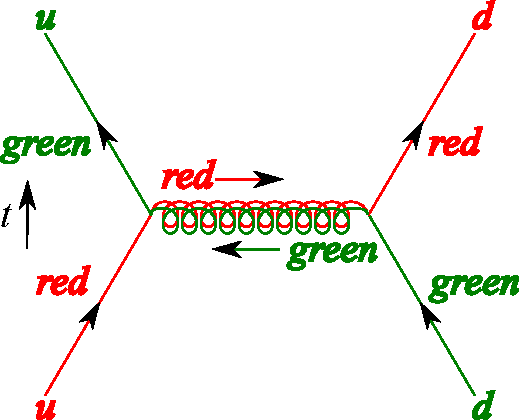
\includegraphics{qcd} % In qcd.svg as a layer
  \caption{Quark--gluon interaction}
  \label{fig:qcd}
\end{figure}

Mientras que el segundo y tercer término dan lugar a autointeracciones de los gluones como se muestra en la Figura \ref{fig:qcd3gluon}
\begin{figure}
  \centering
  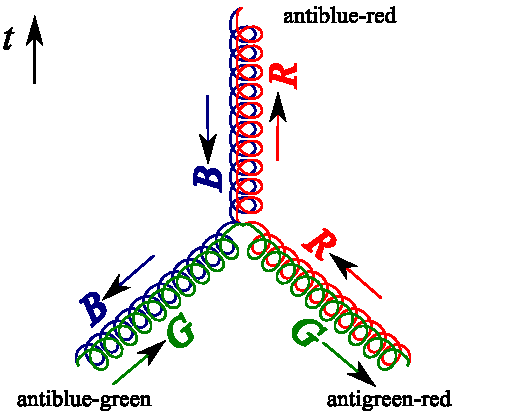
\includegraphics{qcd3gluon}% In qcd.svg as a layer
  \caption{Triple--gluon self--interaction. The anticolors are the colors running back in time.}
  \label{fig:qcd3gluon}
\end{figure}


Todas las interacciones están determinadas en términos de una única constante de acoplamiento $g_s$. Las autointeracciones gauge pueden explicar aspectos de la interacción fuerte como la libertada asintótica, que consiste en que las interacciones fuertes se vuelven más débiles a distancias cortas. 

En términos de índices de color la corriente, y las otras partes del Lagrangiano, pueden escribirse como
\begin{equation}
  \label{eq:223qft}
  J^\mu_a=-g_s\bar{q}^\alpha\gamma^\mu q^\beta\left(\frac{\lambda_a}{2}\right)_{\alpha\beta}.
\end{equation}
Note que tanto para la Electrodinámica Cuántica como para la Cromodinámica Cuántica la corriente $\bar{\psi}\Gamma\psi$ es vectorial. Para las interacciones débiles la estructura es más complicada y requiere un conocimiento más profundo de la ecuación de Dirac y sus soluciones.


\section{Fermiones quirales de cuatro componentes}
\label{sec:ferm-quir-de}
En general un fermion puede descomponerse en sus partes izquierdas y derechas
\begin{align}
  \mathcal{L}  =&i\overline{\psi_R}\gamma^\mu\partial_\mu\psi_R+i\overline{\psi_L}\gamma^\mu\partial_\mu\psi_L-m(\overline{\psi_R}\psi_L+\overline{\psi_L}\psi_R)\,.
\end{align}



En términos de espinores izquierdos y derechos de cuatro componentes la transformación de paridad 
\begin{align}
  \label{eq:220qft}
  t&\to t&\mathbf{x}&\to -\mathbf{x}&\psi_L(t,\mathbf{x})\to&\psi_R(t,-\mathbf{x}),& \psi_R(t,\mathbf{x})&\to\psi_L(t,-\mathbf{x})\nonumber\\
  \partial_0&\to \partial_0&\boldsymbol{\nabla}&\to -\boldsymbol{\nabla}&\psi_L(t,\mathbf{x})\to&\psi_R(t,-\mathbf{x}),& \psi_R(t,\mathbf{x})&\to\psi_L(t,-\mathbf{x})\,.
\end{align}
Además $\mathbf{L}=\mathbf{r}\times \mathbf{p}\to(-\mathbf{r})\times (-\mathbf{p})=\mathbf{L}$, y como $\gamma^\mu$ esta asociado al momento angular intrínsico, entonces también $\gamma^\mu\to\gamma^\mu$


Entonces la transformación de paridad da lugar a (sin tener en cuenta el cambio de argumento en los campos que desaparece en la integral de la Acción)
\begin{align}
  \overline{\psi_R}\gamma^\mu\partial_\mu\psi_R=\overline{\psi_R}\gamma^0\partial_0\psi_R+\overline{\psi_R}\boldsymbol{\gamma}\cdot\boldsymbol{\nabla}\psi_R 
\to&\overline{\psi_L}\gamma^0\partial_0\psi_L-\overline{\psi_L}\boldsymbol{\gamma}\cdot\boldsymbol{\nabla}\psi_L\nonumber\\
=&\overline{\psi_L}\gamma^0\partial_0\psi_L+\overline{\psi_L}\boldsymbol{\gamma}^\dagger\cdot\boldsymbol{\nabla}\psi_L\nonumber\\
=&\overline{\psi_L}\gamma^0\gamma^0\gamma^0\partial_0\psi_L+\overline{\psi_L}\gamma^0\boldsymbol{\gamma}\gamma^0\cdot\boldsymbol{\nabla}\psi_L\nonumber\\
=&\overline{\psi_L}\tilde\gamma^0\partial_0\psi_L+\overline{\psi_L}\tilde{\boldsymbol{\gamma}}\cdot\boldsymbol{\nabla}\psi_L\nonumber\\
=&\overline{\psi_L}\tilde\gamma^\mu\partial_\mu\psi_L\,.
\end{align}
Entonces
\begin{align}
   \mathcal{L}\to\mathcal{L}'=&i\overline{\psi_R}\tilde\gamma^\mu\partial_\mu\psi_R+i\overline{\psi_L}\tilde\gamma^\mu\partial_\mu\psi_L-m(\overline{\psi_R}\psi_L+\overline{\psi_L}\psi_R)\,,
\end{align}
donde $\tilde\gamma^\mu=U\gamma^\mu U^\dagger$, con $U=\gamma^0$. Como las dos representaciones dan lugar a la misma física, podemos decir que la Acción en términos de espinores $L,R$ de cuatro componentes es invariante bajo la transformación de paridad.

La existencia de ambos espinores $\psi_{L,R}$ garantizan que el Lagrangiano de Dirac es invariante bajo la transformación de paridad. 

La corriente de la electrodinámica cuántica en ec.~\eqref{eq:222qft} (o la de la cromodinámica cuántica, ec.~\eqref{eq:223qft}) conservan paridad ya que, siguiendo los mismos pasos que en la ec.~\eqref{eq:221qft}
\begin{align}
  \label{eq:224qft}
  \overline{\psi}\gamma^\mu\psi=\overline{\psi_L}\gamma^\mu\psi_L+\overline{\psi_R}\gamma^\mu\psi_R\to\overline{\psi_L}\tilde{\gamma}^\mu\psi_L+\overline{\psi_R}\tilde{\gamma}^\mu\psi_R\,.
\end{align}
Si para alguna partícula, como es el caso del neutrino, no existe la componente derecha, entonces la correspondiente interacción vectorial viola paridad y no puede tener ni interacciones electromagnéticas ni fuertes, es decir, no se acopla con el fotón o los gluones. Además dicha partícula no puede tener masa de Dirac. En el caso del neutrino esto se entiende pues al no tener carga eléctrica sólo requiere dos grados de libertad independientes.

Definiendo un espinor de  Weyl de dos componentes como
\begin{align*}
  \psi_L=  \begin{pmatrix}
    \widetilde{\psi}_L\\
    0 
  \end{pmatrix}
\end{align*}
Usando la representación de Weyl para las matrices de Dirac
\begin{equation}
  \gamma^\mu=\begin{pmatrix}
    0&\sigma^\mu\\
    \bar{\sigma}^\mu & 0
  \end{pmatrix}
\end{equation}
donde
\begin{align}
  \sigma^\mu&=(\sigma^0,\sigma^1,\sigma^2,\sigma^3)\nonumber\\
  \bar{\sigma}^\mu&=(\sigma^0,-\sigma^1,-\sigma^2,-\sigma^3)\,,
\end{align}
tenemos que
\begin{align*}
  \gamma_5=
  \begin{pmatrix}
    1 &0\\
    0&-1\\
  \end{pmatrix}
\end{align*}
Entonces

Sea
\begin{align}
  P_L\equiv&\frac{1-\gamma_5}{2}\nonumber\\
  P_R\equiv&\frac{1+\gamma_5}{2}\,.
\end{align}
Además
\begin{align}
  \psi_L\equiv P_L\psi\nonumber\\
  \psi_R\equiv P_R\psi\,.
\end{align}
Entonces
\begin{align}
  \psi=\psi_L+\psi_R\,.
\end{align}

Las matrices $P_{L,R}$ tienen las propiedades
\begin{align}
  P_L+P_R&=1 & P_{L,R}^2&=P_{L,R}P_{L,R}=P_{L,R}\nonumber\\
  P_L P_R&=0& P_{L,R}^\dagger&=P_{L,R}\,.
\end{align}
Usando la ec.~(\ref{eq:218qft})
\begin{align}
  P_{L,R}\gamma^\mu=\frac{1\mp\gamma_5}{2}\gamma^\mu=\gamma^\mu\frac{1\pm\gamma_5}{2}=\gamma^\mu P_{R,L}
\end{align}
Para escribir el Lagrangiano en término de los nuevos $\psi_{L,R}$ debemos tener en cuenta que
\begin{align}
  \overline{\psi_{L,R}}=(P_{L,R}\psi)^\dagger\gamma^0=\psi^\dagger P_{L,R}\gamma^0=\psi^\dagger\gamma^0P_{R,L}=\overline{\psi}P_{R,L}
\end{align}
\begin{align}
  \label{eq:221qft}
  \mathcal{L}=&i\overline{\psi}\gamma^\mu\partial_\mu\psi-m\overline{\psi}\psi\nonumber\\
  =&i\overline{\psi}(P_L+P_R)\gamma^\mu\partial_\mu\psi-m\overline{\psi}(P_L+P_R)\psi\nonumber\\
  =&i\overline{\psi}P_L\gamma^\mu\partial_\mu\psi+i\overline{\psi}P_R\gamma^\mu\partial_\mu\psi-m\overline{\psi}P_L\psi-m\overline{\psi}P_R\psi\nonumber\\
  =&i\overline{\psi}P_L P_L\gamma^\mu\partial_\mu\psi+i\overline{\psi}P_R P_R\gamma^\mu\partial_\mu\psi-m\overline{\psi}P_L P_L\psi-m\overline{\psi}P_R P_R\psi\nonumber\\
  =&i\overline{\psi}P_L\gamma^\mu\partial_\mu P_R\psi+i\overline{\psi}P_R\gamma^\mu\partial_\mu P_L\psi-m\overline{\psi}P_L P_L\psi-m\overline{\psi}P_R P_R\psi\nonumber\\
  =&i\overline{\psi_R}\gamma^\mu\partial_\mu\psi_R+i\overline{\psi_L}\gamma^\mu\partial_\mu\psi_L-m(\overline{\psi_R}\psi_L+\overline{\psi_L}\psi_R)\,.
\end{align}
Se puede demostrar como se hace en detalle en \ref{sec:lagrangiano-de-weyl} que en ese caso
\begin{align*}
   \boldsymbol{\sigma}\cdot \mathbf{p}\widetilde{\psi}_{L(R)}=\mp \widetilde{\psi}_{L(R)}
\end{align*}


De otro lado, si una determinada interacción, como es el caso de la interacción débil, solo participa la componente izquierda de la ec.~\eqref{eq:224qft}, está corresponde a una interacción del tipo
\begin{align}
  \overline{\psi}_L\gamma^\mu\psi_L&=\overline{\psi}P_R\gamma^\mu P_L\psi=\overline{\psi}\gamma^\mu P_L\psi\nonumber\\
  &=\overline{\psi}\gamma^\mu\left(\frac{1-\gamma_5}{2}\right)\psi\nonumber\\
  &=\tfrac{1}{2}\overline{\psi}\left(\gamma^\mu-\gamma^\mu\gamma_5\right)\psi\,,
\end{align}
que de acuerdo a la asignación en la Tabla corresponde a una corriente V--A.


\subsection{Ecuaciones de Euler--Lagrange}
\label{sec:ecuaciones-de-euler-1}
Sigiendo los mismos procedimientos anteriores debemos llegar a los siguientes resultados. Para el campo $\Psi$
\begin{align}
  (i\gamma^\mu\mathcal{D}_\mu-m)\Psi=0\,,
\end{align}
\begin{align}
  &\partial_\mu\left[\frac{\partial\mathcal{L}}{\partial\left(\partial_\mu G_\nu^a\right)}\right]-\frac{\partial\mathcal{L}}{\partial G_\nu^a}\nonumber\\
=&\partial_\mu\left\{-  \widetilde{G}^{\mu\nu}_a-\frac{1}{2}g_s f_{dbc}G_b^\rho G^\sigma_c\frac{\partial}{\partial\left(\partial_\mu G_\nu^a\right)}
\left(\partial_\rho G_\sigma^d-\partial_\sigma G_\rho^d\right)\right\}
-g_s\overline{\Psi}\gamma^\nu\frac{\lambda_a}{2}\Psi\nonumber\\
&+\frac{g_s}{2} f^{dbc}\widetilde{G}^{\rho\sigma}_d(\delta_{\rho\nu}\delta_{ba}G^c_\sigma+G^b_\rho\delta_{\sigma\nu}\delta_{ca})
+\frac{g_s}{4}f^{ibc}f_{ide}(g^{\rho\alpha}g^{\sigma\beta}G^b_{\alpha}G^c_\beta G^d_\rho G^e_\sigma)\nonumber\\
  =&\partial_\mu\left\{- \widetilde{G}^{\mu\nu}_a-\frac{1}{2}g_s f_{dbc}G_b^\rho G^\sigma_c
\left(\delta_{\rho\mu}\delta_{\sigma\nu}\delta_{da}-\delta_{\sigma\mu}\delta_{\rho\nu}\delta_{da}\right)\right\}
-g_s\overline{\Psi}\gamma^\nu\frac{\lambda_a}{2}\Psi\nonumber\\
&+\frac{g_s}{2} f^{dac}\widetilde{G}^{\nu\sigma}_dG^c_\sigma
+\frac{g_s}{2} f^{dba}\widetilde{G}^{\rho\nu}_dG^b_\rho\nonumber\\
&+\frac{g_s}{4}f^{ibc}f_{ide}g^{\rho\alpha}g^{\sigma\beta}(\delta_{\alpha\nu}\delta_{ba}G^c_\beta G^d_\rho G^e_\sigma+G^b_{\alpha}\delta_{\beta\nu}\delta_{ca}G^d_\rho G^e_\sigma+G^b_{\alpha}G^c_\beta\delta_{\rho\nu}\delta_{da}G^e_\sigma+G^b_{\alpha}G^c_\beta G^d_\rho\delta_{\sigma\nu}\delta_{ea})\nonumber\\
  =&-\partial_\mu\left\{  \widetilde{G}^{\mu\nu}_a-\frac{1}{2}g_s f^{abc}G_b^\mu G^\nu_c
+\frac{1}{2}g_s f_{abc}G_b^\nu G^\mu_c\right\}
-g_s\overline{\Psi}\gamma^\nu\frac{\lambda_a}{2}\Psi\nonumber\\
&-\frac{g_s}{2} f^{adc}\widetilde{G}^{\nu\sigma}_dG^c_\sigma
-\frac{g_s}{2} f^{adb}\widetilde{G}^{\nu\rho}_dG^b_\rho\nonumber\\
&+\frac{g_s}{4}f^{iac}f_{ide}g^{\rho\nu}g^{\sigma\beta}G^c_\beta G^d_\rho G^e_\sigma
+\frac{g_s}{4}f^{iba}f_{ide}g^{\rho\alpha}g^{\sigma\nu}G^b_{\alpha}G^d_\rho G^e_\sigma
+\frac{g_s}{4}f^{ibc}f_{iae}g^{\nu\alpha}g^{\sigma\beta}G^b_{\alpha}G^c_\beta G^e_\sigma\nonumber\\
&+\frac{g_s}{4}f^{ibc}f_{ida}g^{\rho\alpha}g^{\nu\beta}G^b_{\alpha}G^c_\beta G^d_\rho\,.
\end{align}
Desarrollando los cuatro últimos términos, tenemos

\begin{align}
  &\frac{g_s}{4}f^{iac}f_{ide}g^{\rho\nu}g^{\sigma\beta}G^c_\beta G^d_\rho G^e_\sigma
+\frac{g_s}{4}f^{iba}f_{ide}g^{\rho\alpha}g^{\sigma\nu}G^b_{\alpha}G^d_\rho G^e_\sigma
+\frac{g_s}{4}f^{ibc}f_{iae}g^{\nu\alpha}g^{\sigma\beta}G^b_{\alpha}G^c_\beta G^e_\sigma\nonumber\\
&+\frac{g_s}{4}f^{ibc}f_{ida}g^{\rho\alpha}g^{\nu\beta}G^b_{\alpha}G^c_\beta G^d_\rho\nonumber\\
=&\frac{g_s}{4}f^{iac}f_{ide}G_d^\nu G_c^\mu G^e_\mu
+\frac{g_s}{4}f^{iba}f_{ide}G_e^\nu G_b^{\mu}G^d_\mu
+\frac{g_s}{4}f^{ibc}f_{iae}G_b^{\nu}G_c^\mu G^e_\mu
+\frac{g_s}{4}f^{ibc}f_{ida}G_c^\nu G_b^{\mu}G^d_\mu\nonumber\\
=&  \frac{g_s}{4}f^{dac}f_{dje}G_j^\nu G_c^\mu G^e_\mu
+\frac{g_s}{4}f^{dca}f_{dje}G_e^\nu G_c^{\mu}G^j_\mu
+\frac{g_s}{4}f^{dbc}f_{dae}G_b^{\nu}G_c^\mu G^e_\mu
+\frac{g_s}{4}f^{dbc}f_{dea}G_c^\nu G_b^{\mu}G^e_\mu\nonumber\\
=&  \frac{g_s}{4}f^{dac}f_{dje}G_j^\nu G_c^\mu G^e_\mu
+\frac{g_s}{4}f^{dca}f_{dje}G_e^\nu G_c^{\mu}G^j_\mu
+\frac{g_s}{4}f_{dac}f^{dje}G_j^{\nu}Gc_e^\mu G^c_\mu
+\frac{g_s}{4}f_{dca}f^{dje}G_e^\nu G_j^{\mu}G^c_\mu\nonumber\\
=&  -\frac{g_s}{4}f^{abc}G^b_\mu f_{cej}G_e^\mu G_j^\nu
-\frac{g_s}{4}f^{abc}G^b_{\mu}f_{cej}G_e^\mu G_j^\nu
-\frac{g_s}{4}f_{abc}G^b_\mu f^{cej}G_e^\mu G_j^{\nu}
-\frac{g_s}{4}f_{abc}G^b_\mu f^{cej}G_e^{\mu}G_j^\nu\nonumber\\
=&-g_sf_{abc}G^b_\mu f^{cej}G_e^{\mu}G_j^\nu
\end{align}
Entonces
\begin{align}
    &\partial_\mu\left[\frac{\partial\mathcal{L}}{\partial\left(\partial_\mu G_\nu^a\right)}\right]-\frac{\partial\mathcal{L}}{\partial G_\nu^a}\nonumber\\
    =&\partial_\mu\left(-  \widetilde{G}^{\mu\nu}_a-g_s f^{abc}G_b^\mu G^\nu_c
\right)
-g_s\overline{\Psi}\gamma^\nu\frac{\lambda_a}{2}\Psi
-g_s f^{acd}G^c_\mu\widetilde{G}^{\mu\nu}_d
-g_sf_{acd}G^c_\mu f^{dej}G_e^{\mu}G_j^\nu\nonumber\\
      =&-\partial_\mu{G}^{\mu\nu}_a-g_s f^{acd}G^c_\mu{G}^{\mu\nu}_d
-g_s\overline{\Psi}\gamma^\nu\frac{\lambda_a}{2}\Psi=0\,.
\end{align}
Entonces las Ecuaciones de Euler Lagrange para $G_\nu^a$, son
\begin{align}
\label{eq:Gmuael}
\partial_\mu{G}^{\mu\nu}_a+g_s f^{acd}G^c_\mu{G}^{\mu\nu}_d
=-g_s\overline{\Psi}\gamma^\nu\frac{\lambda_a}{2}\Psi\,.
\end{align}
Definiendo
\begin{align}
J^\mu_a = -g_s\bar{\Psi}\gamma^\mu\frac{\lambda_a}{2}\Psi\,,
\end{align}

La ec.\eqref{eq:Gmuael} puede reescribirse como:
\begin{align}
  \partial_\mu G^{\mu\nu}_a=-g_s\left[f_{abc}G^b_\mu G^{\mu\nu}_c+\bar{\Psi}\gamma^\nu\frac{\lambda_a}{2}\Psi  \right]
\end{align}
y usando el hecho que $\partial_\mu\partial_\nu=\partial_\nu\partial_\mu$:
\begin{align}
  \partial_\nu\partial_\mu G^{\mu\nu}_a=&\partial_\nu\partial_\mu\widetilde{G}^{\mu\nu}+g_s\partial_\nu\partial_\mu\left(f_{abc}G^\mu_bG^\nu_c\right)\nonumber\\
=&0+\frac{1}{2}\left[g_s\partial_\nu\partial_\mu\left(f_{abc}G^\mu_bG^\nu_b\right)+g_s\partial_\nu\partial_\mu\left(f_{abc}G^\mu_bG^\nu_c\right)\right]\nonumber\\
=&\frac{1}{2}\left[g_s\partial_\nu\partial_\mu\left(f_{abc}G^\mu_bG^\nu_b\right)+g_s\partial_\mu\partial_\nu\left(f_{abc}G^\mu_bG^\nu_c\right)\right]\nonumber\\
=&\frac{1}{2}\left[g_s\partial_\nu\partial_\mu\left(f_{abc}G^\mu_bG^\nu_b\right)+g_s\partial_\nu\partial_\mu\left(f_{acb}G^\nu_cG^\mu_b\right)\right]\nonumber\\
=&\frac{1}{2}\left[g_s\partial_\nu\partial_\mu\left(f_{abc}G^\mu_bG^\nu_b\right)-g_s\partial_\mu\partial_\nu\left(f_{abc}G^\mu_bG^\nu_c\right)\right]\nonumber\\
=&0\,,
\end{align}
como en el caso Abeliano, tenemos la corriente conservada
\begin{align}
  \partial_\nu j^\nu=0\,,
\end{align}
donde
\begin{align}
\label{eq:jnuqcd}
  j^\nu_a=&-g_s\left[f_{abc}G^b_\mu G^{\mu\nu}_c+\bar{\Psi}\gamma^\nu\frac{\lambda_a}{2}\Psi  \right]\,.
\end{align}

El primer término corresponde a las autointeracciones y el segundo a la corriente de color generada por los quarks.


\subsection{Derivada covariante adjunta}
Toda el algebra de $SU(3)$ se puede escribir en notación vectorial en términos de vectores de 8 componentes asociados al espacio de los generadores de $SU(3)$. Este nos permitira entender como las autointeracciones gauge emergen también de la derivada covariante cuando se escribe en la representación adjunta de $SU(3)$.

Definiendo el producto vectorial de $SU(3)$ como
\begin{align}
  \left(\mathbf{A}\times \mathbf{B}\right)_a=f_{abc}A^b B^c\,,
\end{align}
si $\mathbf{G}^\mu$ es un vector en el espacio $SU(3)$ con las 8 componentes $G^\mu_a$, entonces podemos escribir \eqref{eq:gmutrinf} como
\begin{align}
  \mathbf{G}_\mu\to\mathbf{G}'_\mu=\mathbf{G}_\mu+\frac{1}{g_s}\partial_\mu\boldsymbol{\theta}+\mathbf{G}_\mu\times \boldsymbol{\theta}\,.
\end{align}

Podemos escribir también la ec.~\eqref{eq:258qft} en términos de vectores en el espacio $SU(3)$ como:
\begin{align}
  \mathbf{G}^{\mu\nu}=\partial^\mu \mathbf{G}^\nu-\partial^\nu \mathbf{G}^\mu+g_s \mathbf{G}^\mu\times  \mathbf{G}^\nu\,,
\end{align}
donde $\mathbf{G}^{\mu\nu}$ es el vector en el espacio $SU(3)$ con las 8 componentes $G^{\mu\nu}_a$.



De igual forma, podemos escribir \eqref{eq:Gmuael} en forma vectorial como
\begin{align}
  \partial_\mu\mathbf{G}^{\mu\nu}+g_s \mathbf{G}_\mu\times \mathbf{G}^{\mu\nu}=\mathbf{J}^\nu
\end{align}
y la corriente conservada como
\begin{align}
 \mathbf{j}^\nu =&-g_s\left[-\mathbf{G}^{\mu\nu}\times \mathbf{G}_\nu^b+\bar{\Psi}\gamma^\nu\frac{\boldsymbol{\lambda}}{2}\Psi  \right]\,.
\end{align}

Como ${G}^{\mu\nu}$ es una matrix $8\times 8$, su derivada covariante debe estar en la representación adjunta de $SU(3)$
\begin{align}
  \left(\Lambda^a\right)_{bc}=-i\left(f^a\right)_{bc}\,,
\end{align}
con
\begin{align}
  \left[\Lambda^a,\Lambda^b\right]=i f_{abc}\Lambda^c\,.
\end{align}
En esta representación la derivada covariante queda
\begin{align}
  \mathcal{D}_\mu=\partial_\mu-i g_s\Lambda_aG_\mu^a
\end{align}
En componentes
\begin{align}
  \left(\mathcal{D}_\mu\right)_{ab}=&\delta_{ab}\partial_\mu-i g_s (\Lambda^c)_{ab}G_\mu^c\nonumber\\
  =&\delta_{ab}\partial_\mu-g_s f_{cab}G_\mu^c\nonumber\\
  =&\delta_{ab}\partial_\mu+g_s f_{acb}G_\mu^c\,.
\end{align}

Aplicada sobre la componente $G^{\mu\nu}_b$, queda
\begin{align}
 \left(\mathcal{D}_\mu\right)_{ab}G^{\mu\nu}_b  =&\delta_{ab}\partial_\mu G^{\mu\nu}_b+g_s f_{acb}G_\mu^cG^{\mu\nu}_b\nonumber\\
 \left(\mathcal{D}_\mu\right)_{ab}G^{\mu\nu}_b  =&\partial_\mu G^{\mu\nu}_a+g_s \left(\mathbf{G}_\mu\times \mathbf{G}^{\mu\nu}\right)_a\nonumber\\
 \left(\mathcal{D}_\mu\mathbf{G}^{\mu\nu}\right)_a  =&\partial_\mu\mathbf{G}^{\mu\nu}_a+g_s \left(\mathbf{G}_\mu\times \mathbf{G}^{\mu\nu}\right)_a\,,
\end{align}
podemos escribir la derivada covariante de $\mathbf{G}^{\mu\nu}=\left(G^{\mu\nu}_1,\cdots,G^{\mu\nu}_8\right)$ como
\begin{align}
  \mathcal{D}_\mu \mathbf{G}^{\mu\nu}=&\partial_\mu\mathbf{G}^{\mu\nu}+g_s \mathbf{G}_\mu\times \mathbf{G}^{\mu\nu}\,.
\end{align}


Entonces las las Ecuaciones de Euler Lagrange para $G_{\mu\nu}^a$, en \eqref{eq:Gmuael} se pueden escribir como
\begin{align}
  \mathcal{D}_\mu \mathbf{G}^{\mu\nu}=&\mathbf{J}^\nu\,,
\end{align}
donde el vector en espacio $SU(3)$ $\mathbf{J}^\nu$, tiene por componentes
  \begin{align}
J^\mu_a = -g_s\bar{\Psi}\gamma^\mu\frac{\lambda_a}{2}\Psi\,.
\end{align}

Para escribir el Lagrangiano en forma vectorial en el espacio $SU(3)$, debemos reescribir la transformación gauge de $G_{\mu\nu}$ en términos de vectores de $SU(3)$. Como
\begin{align}
  {G}_{\mu\nu}\to{G}'_{\mu\nu}=&U G_{\mu\nu} U^{\dagger}\nonumber\\
  =&(1+i\theta_b\Lambda^b)\Lambda^cG^c_{\mu\nu}(1-i\theta_b\Lambda^b)
\end{align}
podemos realizar los mismos pasos que en \eqref{eq:Gmuinv}. El resultado es
\begin{align}
    G_{\mu\nu}^a\to {G'}_{\mu\nu}^a\approx&G_{\mu\nu}^a+f^{abc}G_{\mu\nu}^b\theta^c\,.
\end{align}
Note que en el caso Abeliano $f_{abc}=0$, el tensor correspondiente es invariante gauge, como ocurre el caso electromagnético. En notación de vectores de $SU(3)$:
\begin{align}
  \mathbf{G}_{\mu\nu}\to\mathbf{G}'_{\mu\nu}\approx\mathbf{G}_{\mu\nu}+\mathbf{G}_{\mu\nu}\times \boldsymbol{\theta}\,.
\end{align}
Utilizando la propiedad cíclica del triple producto escalar
\begin{align}
  \mathbf{A}\cdot(\mathbf{B}\times \mathbf{C})=\mathbf{B}\cdot(\mathbf{C}\times \mathbf{A})=\mathbf{C}\cdot(\mathbf{A}\times \mathbf{B})\,,
\end{align}
podemos construir el invariante

\begin{align}
  G^{\mu\nu}_aG^a_{\mu\nu}=\mathbf{G}^{\mu\nu}\cdot\mathbf{G}_{\mu\nu}\to{\mathbf{G}'}^{\mu\nu}\cdot\mathbf{G}'_{\mu\nu}\approx&
  \mathbf{G}^{\mu\nu}\cdot\mathbf{G}_{\mu\nu}+\mathbf{G}^{\mu\nu}\cdot\left(\mathbf{G}_{\mu\nu}\times \boldsymbol{\theta}\right)
+\left(\mathbf{G}^{\mu\nu}\times \boldsymbol{\theta}\right)\cdot\mathbf{G}_{\mu\nu}\nonumber\\
=&\mathbf{G}^{\mu\nu}\cdot\mathbf{G}_{\mu\nu}+\mathbf{G}_{\mu\nu}\cdot\left(\boldsymbol{\theta}\times \mathbf{G}^{\mu\nu}\right)
+\left(\mathbf{G}^{\mu\nu}\times \boldsymbol{\theta}\right)\cdot\mathbf{G}_{\mu\nu}\nonumber\\
=& \mathbf{G}^{\mu\nu}\cdot\mathbf{G}_{\mu\nu}-\left(\mathbf{G}^{\mu\nu}\times \boldsymbol{\theta}\right)\cdot\mathbf{G}_{\mu\nu}
+\left(\mathbf{G}^{\mu\nu}\times \boldsymbol{\theta}\right)\cdot\mathbf{G}_{\mu\nu}\nonumber\\
=&\mathbf{G}^{\mu\nu}\cdot\mathbf{G}_{\mu\nu}\,.
\end{align}

El Lagrangiano de la QCD escrito en forma de vectores de $SU(3)$ es
\begin{align}
  \mathcal{L}=i\bar{\Psi}\gamma^\mu\left(\partial_\mu-i g_s\frac{\boldsymbol{\lambda}}{2}\cdot\mathbf{G}_\mu\right)\Psi
  -m\bar{\Psi}\Psi- \frac{1}{4}\mathbf{G}^{\mu\nu}\cdot\mathbf{G}_{\mu\nu}\,.
\end{align}
El Lagrangiano para los campos gauge, el cual puede generalizarse para cualquier teoría $SU(N)$, es
\begin{align}
  \mathcal{L}_{\text{gluon}}=\mathcal{L}_{\text{gauge}}+\mathcal{L}_{\text{SI}}=- \frac{1}{4}\mathbf{G}^{\mu\nu}\cdot\mathbf{G}_{\mu\nu}-\mathbf{J}_\nu\cdot\mathbf{G}^\nu\,,
\end{align}
Da lugar la ecuaciones de Maxwell pero con la derivada normal reemplzada por la derivada covariante 
\begin{align}
  \mathcal{D}_\mu \mathbf{G}^{\mu\nu}=&\mathbf{J}^\nu\,,
\end{align}
donde
\begin{align}
    \mathcal{D}_\mu \mathbf{G}^{\mu\nu}=&\partial_\mu\mathbf{G}^{\mu\nu}+g_s \mathbf{G}_\mu\times \mathbf{G}^{\mu\nu}\,.
\end{align}
Note que en el caso Abeliano, $U(1)$, la derivada covariante del tensor de campo se reduce a la derivada normal de dicho tensor. El término extra en la derivada covariante da lugar a las autointeracciones de los campos gauge.

\begin{itemize}
\item \textbf{Ejercicio:}

Muestre que la derivada covariante de $\mathbf{G}^{\mu\nu}$, transforma como $\mathbf{G}^{\mu\nu}$.
\end{itemize}

% \begin{align}
%   \mathcal{D}_\mu G^{\mu\nu}=&\left(\partial_\mu-i g_s G_\mu\right)G^{\mu\nu}\nonumber\\
%   =&\partial_\mu G^{\mu\nu}-i g_s G_\mu G^{\mu\nu}\nonumber\\
%   =&\Lambda^a\partial_\mu G^{\mu\nu}_a-i g_s \Lambda_b\Lambda^cG_\mu^bG^{\mu\nu}_c
% \end{align}


\section{Ecuaci\'on de klein-Gordon}
\label{sec:ecuacion-de-klein}
%to_en: From the scalar component we obtain from eq.~\eqref{eq:27}, with the Lagrangian for the Klein-Gordon equation for a real scalar field $\phi=A^0$
La interacci\'on entre un prot\'on y un neutr\'on fue determinada experimentalmente por Tomonaga en 1934 \cite{history}
\begin{align}
\label{eq:243}
  V(r)={A}\frac{e^{-r/\Lambda }}{r}\,,
\end{align}
con
\begin{align}
  \label{eq:245}
  \Lambda\approx1/(7\times10^{12}\,\text{cm}^{-1})=1.43\times10^{-13}\,\text{cm}=1.43\times10^{-15}\,\text{m}\,.
\end{align}
Consideremos el principio de incertidumbre
\begin{align}
  \Delta x\, \Delta p &\geq \frac{\hbar}{2}\nonumber\\
\Delta t\, \Delta E&\geq\frac{\hbar}{2}\,.
\end{align}
La segunda relaci\'on de incertidumbre
aplicada a la ecuación de Klein-Gordon~\cite{Aitchison:2003tq}, brinda un nuevo entendimiento de la relaci\'on entre el rango y la masa en ec.~\eqref{eq:243}. $\Delta t$ es el tiempo que el sistema cu\'antico interact\'ua con el aparato de medida y $\Delta E=\hbar/(2\Delta t)$ es el error m\'\i nimo que se obtiene en la medida de la energ\'\i a, tal que $E=E_0\pm\Delta E$. Es decir, para medir la energ\'\i a con una precisi\'on $\Delta E$, uno necesita un tiempo mayor que $\hbar/(2\Delta E)$.

Si $\Delta E< mc^2$ eso quiere decir que podemos medir la cantidad $mc^2$ con alguna certeza. Es decir que una part\'\i cula de masa $m$ se puede llegar a observar. Si $\Delta E>mc^2$ entonces una part\'\i cula de masa $m$ puede existir durante un tiempo $\Delta t$. A tal part\'\i cula se le llama virtual porque no es observable. 

El momentum de una part\'\i cula de n\'umero de onda $k$ es $p=\hbar k$, de modo que la incertidumbre en el momentum para una part\'\i cula relativista es
\begin{align}
  \Delta p=\hbar\, \Delta k \approx\hbar\, \frac{\Delta\omega}{c}=\frac{\Delta E}{c}
\end{align}

Si la masa de la part\'\i cula es cero entonces $E$ puede tender a cero, que corresponde al caso de un part\'\i cula no masiva con un momentum tendiendo a cero. La cantidad por la cual la conservaci\'on de energ\'\i a es violada, $\Delta E$, tambi\'en puede llegar a ser muy peque\~na. De modo que un fot\'on virtual de frecuencia muy baja puede existir durante un tiempo casi infinito. Durante ese tiempo un fot\'on viajando a la velocidad de la luz podr\'\i a viajar una distancia casi infinita y puede dar cuenta de una interacci\'on de rango infinito. 

Sin embargo, para una part\'\i cula de masa $m$. La violaci\'on de energ\'\i a para producir esta debe ser de al menos $mc^2$, o $\Delta E>mc^2$. Por el principio de incertidumbre la m\'axima distancia que puede recorrer es $\Lambda=c\Delta t$

\begin{align}
\label{eq:244}
  \Lambda \geq & \frac{\hbar c}{2\Delta E}\nonumber\\
  \geq &\frac{c\hbar}{2mc^2}\nonumber\\
  \geq &\frac{\hbar}{2mc}\nonumber\\
  \geq &\frac{1}{2m}\qquad\text{Natural Units} \,.
\end{align}

De la componente escalar de la ecuaci\'on de Proca, \eqref{eq:27}, obtenemos la ecuaci\'on de Klein--Gordon para un campo escalar real $\phi=A^0$,
\begin{align}
  \label{eq:29}
  \mathcal{L}=&\frac{1}{2}\partial^\mu\phi\partial_\mu\phi-\frac{1}{2}m^2\phi^2+\rho\phi
\end{align}
Donde $\rho$ es la densidad de carga que actua como fuente del campo $\phi$.

%to_en: Later we will discuss in detail why $m$ corresponds to the mass of the particle. The idea is that $\phi$ has excitations around the minimum of the potential $V=(1/2)m^2\phi^2$ that have some harmonic oscillator energy, and this energy is equivalent to mass. Note that $m^2\lt 0$ cannot be interpreted as mass. In this case $\phi$ will describe excitations around the flat part of the potential. Since this excitations do not cost energy, they correspond to a non-massive particle.
Posteriormente discutiremos en detalles porque $m$ corresponde a la masa de la part\'\i cula. La idea b\'asica es que $\phi$ tiene excitaciones alrededor del m\'\i nimo del potencial $V=(1/2)m^2\phi^2$ que corresponde a la energ\'\i a de un oscilador arm\'onico. Esta energ\'\i a es equivalente a masa. Note que $m^2\lt 0$ no puede interpretarse como masa. En este caso $\phi$ describir\'a excitaciones alrededor de la parte plana del potencial. Como estas excitaciones no cuestan energ\'\i a, corresponde a una part\'\i cula sin masa. 

%to_en: The field $\phi$ can be thought of as arising from a source in much the same way as the electromagnetic fields arise from charged particles; as for the electromagnetism, en esta secci\'on we can consider the fields without concerning ourselves with the sources. 
El campo $\phi$ puede pensarse como proveniente de una fuente de la misma manera como el campo electromagn\'etico surge de part\'\i culas cargadas. Como en el caso del electromagnetismo, en esta secci\'on podemos considerar los campos sin preocuparnos de las fuentes. 
En tal caso tendremos una teor\'\i a en la cual el campo escalar juega el papel de part\'\i cula mediadora de la interacci\'on.

Si el campo escalar se generaliza para que pueda tener otros n\'umeros
cu\'anticos, como carga el\'ectrica, entonces estos pueden ser las fuentes
de las respectivas cargas y corrientes en la ecuaciones para campos
vectoriales. Esto se estudiar\'a en la
secci\'on~\ref{sec:camp-escal-compl}. En tal caso podr\'\i amos tener por
ejemplo ``\'atomos'' formados de part\'\i culas escalares que se excitan
emitiendo fotones.


En las secciones~\ref{sec:ecuac-covar} y \ref{sec:ecuacion-de-proca},
hemos visto que el Lagrangiano en ec.~\eqref{eq:29} da lugar a las
ecuaciones de Klein-Gordon en presencia de una densidad de carga
\begin{equation}
  \label{eq:30}
  (\Box+m^2)\phi=\rho
\end{equation}
De acuerdo a la ec.~\eqref{eq:28}, tenemos
\begin{align}
\mathcal{L}_{\text{free}}&=\frac{1}{2}\partial_\mu\phi\partial_\mu\phi-\frac{1}{2} m^2\phi^2\nonumber\\
\label{eq:31}
\mathcal{L}_{\text{int}}&=\rho\phi
\end{align}
En analog\'\i a con el electromagn\'etismo donde las densidades de carga y
corrientes son la fuente del campo $A^\mu$, podemos pensar en $\rho$ como
la fuente del campo $\phi$. En el caso del electromagnetismo el an\'alisis
de las ecuaciones de Maxwell en forma covariante,
ec.~\eqref{eq:nohomME2}, para las componentes $A^0$ y $J^0$, en el
gauge de Coulomb:
\begin{equation}
  \label{eq:32}
  \boldsymbol{\nabla}\cdot\mathbf{A}=0,
\end{equation}
da lugar a la Ley de Coulomb, que corresponde a una interacci\'on de
rango infinito \cite{Gross}. Veremos a continuaci\'on que un an\'alisis
similar para un campo escalar masivo (o para la componente cero de un
campo vectorial masivo) da lugar a una interacci\'on de corto rango.

Consideremos el caso m\'as simple de una fuente puntual para el campo
$\phi$:
\begin{equation}
  \label{eq:33}
  \rho(x)=g\delta(\mathbf{x})
\end{equation}
donde $g$ es una constante. Entonces $\rho$ es independiente del tiempo y
genera un campo (un potencial) independiente del tiempo. Entonces,
como:
\begin{equation*}
  \frac{\partial\phi}{\partial t}=0,
\end{equation*}
tenemos
\begin{equation}
  \label{eq:34}
  (-\nabla^2+m^2)\phi(\mathbf{x})=g\delta(\mathbf{x})
\end{equation}
Para resolver la ecuaci\'on diferencial es m\'as conveniente transformar
$\phi(\mathbf{x})$ al espacio de momentos. Su transformada de Fourier es
\begin{equation}
  \label{eq:35}
  \phi(\mathbf{x})=\frac{1}{(2\pi)^{3/2}}\int d^3k\,e^{i\mathbf{k}\cdot\mathbf{x}}\tilde\phi(\mathbf{k}).
\end{equation}
La transformada inversa es
\begin{equation}
  \label{eq:36}
  \tilde\phi(\mathbf{k})=\frac{1}{(2\pi)^{3/2}}\int d^3x\,e^{-i\mathbf{k}\cdot\mathbf{x}}\phi(\mathbf{x}).
\end{equation}
Ademas tenemos la propiedad
\begin{equation}
  \delta(\mathbf{x})=\frac{1}{(2\pi)^3}\int d^3k\,e^{i\mathbf{k}\cdot\mathbf{x}}.
\end{equation}
Reemplazando ec.~\eqref{eq:35} en \eqref{eq:34}, tenemos
\begin{align}
\frac{1}{(2\pi)^{3/2}}\int d^3k(\mathbf{k}^2+m^2)e^{i\mathbf{k}\cdot\mathbf{x}}\tilde\phi(\mathbf{k})&=g\delta(\mathbf{x})\nonumber\\
&=\frac{g}{(2\pi)^3}\int d^3k\,e^{i\mathbf{k}\cdot\mathbf{x}}\nonumber\\
(\mathbf{k}^2+m^2)\tilde\phi(\mathbf{k})&=\frac{g}{(2\pi)^{3/2}}.\nonumber
\end{align}
Entonces
\begin{equation}
  \tilde\phi(\mathbf{k})=\frac{g}{(2\pi)^{3/2}}\frac{1}{\mathbf{k}^2+m^2}.
\end{equation}
Reemplazando en la ec.~\eqref{eq:35} y definiendo $r\equiv|\mathbf{x}|$
\begin{align}
  \phi(\mathbf{x})=&\frac{1}{(2\pi)^{3/2}}\int d^3k\,e^{i\mathbf{k}\cdot\mathbf{x}}
  \left[
    \frac{g}{(2\pi)^{3/2}}\frac{1}{\mathbf{k}^2+m^2}
  \right]\nonumber\\
=&\frac{g}{(2\pi)^{3}}\int d^3k
    \frac{e^{i\mathbf{k}\cdot\mathbf{x}}}{\mathbf{k}^2+m^2}\nonumber\\
=&\frac{g}{(2\pi)^{3}}2\pi\int_0^\infty d|\mathbf{k}|
    \frac{\mathbf{k}^2}{\mathbf{k}^2+m^2}\int_0^\pi e^{i|\mathbf{k}|r\cos\theta}\sen\theta\,d\theta\nonumber
\end{align}
Haciendo el cambio de variables $u=\cos\theta$, $du=-\sin\theta\,d\theta$,
\begin{align}
  \phi(\mathbf{x})=&-\frac{g}{(2\pi)^2}\int_0^\infty d|\mathbf{k}|
    \frac{\mathbf{k}^2}{\mathbf{k}^2+m^2}\int_{1}^{-1}e^{i|\mathbf{k}|ru}du,\nonumber\\
  \phi(\mathbf{x})=&\frac{g}{(2\pi)^2}\int_0^\infty d|\mathbf{k}|
    \frac{\mathbf{k}^2}{\mathbf{k}^2+m^2}\int_{-1}^1e^{i|\mathbf{k}|ru}du.
\end{align}
%\textbf{check minus sign!} 
Ya que  
\begin{equation*}
  \int_{-1}^1e^{i|\mathbf{k}|ru}du=\frac{e^{i|\mathbf{k}|r}-e^{-i|\mathbf{k}|r}}{i|\mathbf{k}|r}
\end{equation*}
\begin{align}
  \phi(\mathbf{x})=&\frac{g}{i(2\pi)^2r}\int_0^\infty d|\mathbf{k}|\,|\mathbf{k}|
    \frac{e^{i|\mathbf{k}|r}-e^{-i|\mathbf{k}|r}}{\mathbf{k}^2+m^2}\nonumber\\
    =&\frac{g}{i(2\pi)^2r}\left(\int_0^\infty d|\mathbf{k}|\,|\mathbf{k}|
\frac{e^{i|\mathbf{k}|r}}{\mathbf{k}^2+m^2}-\int_0^\infty d|\mathbf{k}|\,|\mathbf{k}|
\frac{e^{-i|\mathbf{k}|r}}{\mathbf{k}^2+m^2}\right)\nonumber\\
=&\frac{g}{i(2\pi)^2r}\left(\int_0^\infty d|\mathbf{k}|\,|\mathbf{k}|
\frac{e^{i|\mathbf{k}|r}}{\mathbf{k}^2+m^2}-\underbrace{\int_0^{-\infty}d|\mathbf{k}|\,|\mathbf{k}|
\frac{e^{i|\mathbf{k}|r}}{\mathbf{k}^2+m^2}}_{|\mathbf{k}|\to-|\mathbf{k}|}\right)\nonumber\\
=&\frac{g}{i(2\pi)^2r}\int_{-\infty}^\infty d|\mathbf{k}|\,|\mathbf{k}|
\frac{e^{i|\mathbf{k}|r}}{\mathbf{k}^2+m^2}\nonumber\\
\label{eq:37}
    =&\frac{g}{i(2\pi)^2r}\int_{-\infty}^\infty d|\mathbf{k}|
    \frac{|\mathbf{k}|e^{i|\mathbf{k}|r}}{(|\mathbf{k}|+im)(|\mathbf{k}|-im)}
\end{align}
Definiendo
\begin{equation*}
  f(z)=\frac{ze^{izr}}{z+im}
\end{equation*}
y usando la integral de Cauchy para el contorno correspondiente al semiplano positivo que incluye el polo en $z=im$
\begin{equation}
  \int_C\frac{f(z)}{z-im}dz=2\pi if(im)=2\pi i\frac{im\,e^{-mr}}{2im}=\pi i\,e^{-mr}
\end{equation}
tenemos que
\begin{equation}
 \label{eq:38}
  \phi(\mathbf{x})=\frac{g}{4\pi}\frac{e^{-mr}}{r}
\end{equation}

A la luz de la interacci\'on fuerte, un prot\'on y un neutr\'on son
indistinguibles y son llamados nucleones. En primera aproximaci\'on la
interacci\'on fuerte puede ser tratada como una interacci\'on de Yukawa en
el rango de los fermis entre los nucleones, mediada por mesones, como el pi\'on. Ver sec. 2.2 de \cite{Aitchison:2003tq}.


Para ver esto considere un nucle\'on como fuente de un mes\'on
intermediario. De acuerdo a la ec.~(\ref{eq:38}),
\begin{align}
  \phi(\mathbf{x})&=\frac{g}{4\pi}\frac{e^{-m|\mathbf{x}|}}{|\mathbf{x}|}\nonumber\\
  &=\frac{1}{4\pi}\int d^3x'g\,\delta(\mathbf{x}')\frac{e^{-m|\mathbf{x}-\mathbf{x}'|}}{|\mathbf{x}-\mathbf{x}'|}\nonumber\\
  &=\frac{1}{4\pi}\int d^3x'\rho(\mathbf{x}')\frac{e^{-m|\mathbf{x}-\mathbf{x}'|}}{|\mathbf{x}-\mathbf{x}'|}
\end{align}

\begin{equation}
  \mathcal{L}_{\text{int}}=\phi(\mathbf{x})\rho(\mathbf{x})=\frac{1}{4\pi}\int d^3x'\rho(\mathbf{x})\rho(\mathbf{x}')\frac{e^{-m|\mathbf{x}-\mathbf{x}'|}}{|\mathbf{x}-\mathbf{x}'|}
\end{equation}
\begin{align}
  \mathcal{H}_{\text{int}}&=\frac{\partial\mathcal{L}_{\text{int}}}{\partial(\partial\phi/\partial t)}\frac{\partial\phi}{\partial t}-\mathcal{L}_{\text{int}}\nonumber\\
  &=-\mathcal{L}_{\text{int}}\nonumber\\
  &=-\frac{1}{4\pi}\int d^3x'\rho(\mathbf{x})\rho(\mathbf{x}')\frac{e^{-m|\mathbf{x}-\mathbf{x}'|}}{|\mathbf{x}-\mathbf{x}'|}
\end{align}
\begin{equation}
  \label{eq:39}
  H_{\text{int}}=-\frac{1}{4\pi}\int d^3x\,d^3x'\rho(\mathbf{x})\rho(\mathbf{x}')\frac{e^{-m|\mathbf{x}-\mathbf{x}'|}}{|\mathbf{x}-\mathbf{x}'|}
\end{equation}
El Hamiltoniano de interacci\'on en ec.~(\ref{eq:39}) representa la
interacci\'on entre dos nucleones mediante el intercambio de un mes\'on.
En forma an\'aloga a como dos electrones intercambian un fot\'on mediante
la interacci\'on electromagn\'etica. En el caso de $m=0$,
$H_{\text{int}}$, corresponde a la de energ\'\i a potencial de Coulomb. El
potencial por unidad de carga al cuadrado, puede escribirse como
\begin{equation}
  \label{eq:40}
    V(r)=-\frac{1}{4\pi}\frac{e^{-mr}}{r}
\end{equation}
El potencial en (\ref{eq:40}) recibe el nombre de \emph{potencial de
  Yukawa} y corresponde a una interacci\'on de rango $r\sim1/m$. 

Comparando con la ec.~(\ref{eq:243}) tenemos
\begin{align}
  m\approx&\frac{1}{\Lambda}
\end{align}
que es compatible con la ec.~\eqref{eq:244}. Usando el valor medido de $\Lambda$ en la ec.~\eqref{eq:245}
\begin{align}
  m\approx&\frac{1}{1.43\times10^{-15}m}\frac{1.973\times10^{-16}\,\text{m}}{\text{GeV}^{-1}}\nonumber\\
  \approx&138\,\text{MeV}
\end{align}
La masa del pion $\pi^0$, es $m_{\pi^0}=134.8766(6)\,$MeV.



En el caso general tenemos que $\phi(x)$ satisface la ecuaci\'on de Klein-Gordon en el espacio libre, ec.~\eqref{eq:30}
\begin{equation}
    (\frac{\partial^2}{\partial t^2}-\nabla^2+m^2)\phi=0
\end{equation}
con soluci\'on, 
\begin{equation}
  \phi\propto\exp(i\mathbf{k}\cdot\mathbf{x}-i\omega t)
\end{equation}
que, consistente con la discusi\'on en la secci\'on~\ref{sec:srn}, ec.\eqref{eq:k-gpmu}, da lugar a la condici\'on 
\begin{equation}
  m^2=\omega^2-\mathbf{k}^2.
\end{equation}
De este modo $m$, puede interpretarse como la masa de la part\'\i cula $\phi$.

Para complementar la discusi\'on, condere el caso de un aparato de medida con el m\'\i nimo requerimiento para descubrir el $\pi^0$.
El tiempo que el $\pi^0$ tarda en crurzar del prot\'on al nucle\'on debe ser al menos de $r/c$. El aparato de medida debe operar a una escala de tiempos
\begin{align}
  \Delta t<\frac{r}{c}\,.
\end{align}
La incertidumbre en la enrg\'\i a ser\'a
\begin{align}
  \Delta E\geq \frac{\hbar}{2\Delta t}=\frac{\hbar c}{2r}\,.
\end{align}
Reemplazando $\Delta E=\frac{1}{2}m c^2$ para que la medida $E\pm\Delta E$ sea significativa a dos $\sigma$, tenemos que
\begin{align}
  r\geq \frac{\hbar}{ m c}\,.
\end{align}
De este modo $r$ es la medidad de la separaci\'on entre $n$ y $p$, tal que en el tiempo disponible, el $\pi^0$ pueda robar la energ\'\i a necesaria para llegar a existir y cruzar de uno a otro. Usando $m=138\,$MeV, tenemos 
\begin{align}
  r\geq\frac{1}{0.138}\,\text{GeV}^{-1}\times\frac{1.973\times10^{-16}\,\text{m}}{\text{GeV}^{-1}}=1.43\times10^{-15}\,\text{m}.
\end{align}
El valor obtenido de $\Lambda$ es compatible con $r$. $\Lambda$ es el rango efectivo de la fuerza asociada. 
A continuaci\'on Yukawa considero la posibilidad de que el quantum $\phi$ pudiera ser emitido en la transici\'on $n\to p$, a trav\'es del proceso
\begin{equation}
  \label{eq:154}
  n\to p+\phi^-
\end{equation}
donde la conservaci\'on de la carga determina la carga de $\phi^-$. Sin embargo el proceso viola la conservaci\'on de la energ\'\i a ya que $m_n=939.565\;56(81)\,$MeV, $m_p=938.272\;013(23)\,$MeV, de modo que $m_n\lt m_p+m_\phi$, si $m_\phi\sim100\,$MeV, as\'\i{} esto no puede ocurrir como un proceso real de emissi\'on. Sin embargo, Yukawa not\'o que si \eqref{eq:154} se combina con el proceso inverso
\begin{equation}
  p+\phi^-\to n
\end{equation}
entonces una interacci\'on $n$--$p$ podr\'\i a tomar lugar a trav\'es del mecanismo mostrado en la figura \ref{fig:n-p}(a). Es decir a trav\'es del intercambio de un quantum $\phi^-$. El otro diagrama compatible con la conservaci\'on de la carga tambi\'en aparece en la figura
%noinstiki
\begin{figure} %noinstiki

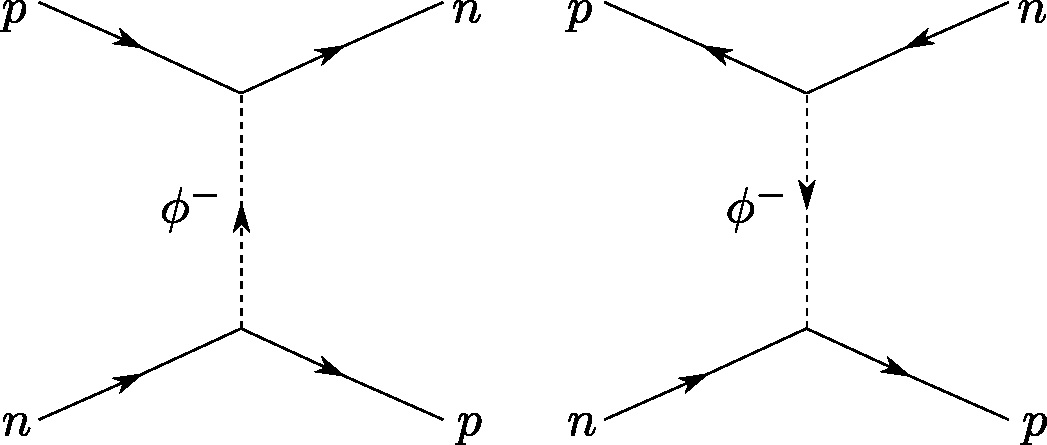
\includegraphics{yukawa-schange} %noinstiki
  \caption{Intercambio de Yukawa de un s\'olo $\phi$} %noinstiki
\label{fig:n-p} %noinstiki
\end{figure} %noinstiki<div id="fig:n-p">Figura: Intercambio de Yukawa</div>
%noinstiki![yukawa-schange](http://gfif.udea.edu.co/figfs/yukawa-schange.png)
%noinstiki


En el espacio de momentos, la cantidad relevante que representa el
intercambio de piones, es la que aparece en la ec.~(\ref{eq:37}) y se
conoce como el \emph{propagador}:
\begin{equation}
\text{propagador:}\qquad \frac{1}{\mathbf{k}^2-m^2}
\end{equation}
En el caso electromagn\'etico tendremos simplemente
\begin{equation}
  1/\mathbf{k}^2.
\end{equation}
Para part\'\i culas $\alpha$ incidiendo sobre un metal y siendo dispersadas por un \'angulo $\theta$ entre $\mathbf{q}$ y $\mathbf{q}'$, tal que se satisface la condici\'on de dispersi\'on el\'astica $\mathbf{q}^2={\mathbf{q}'}^2$ (dispersi\'on de Rutherford)
\begin{align}
  \mathbf{k}^2=(\mathbf{q}-\mathbf{q}')^2=2\mathbf{q}^2(1-\cos\theta)=4\mathbf{q}^2\sin^2\frac{\theta}{2}
\end{align}
Entonces
\begin{align}
  \text{cross section}&\propto\frac{1}{\mathbf{k}^2}\nonumber\\
  &\propto\sin^{-4}\frac{\theta}{2},
\end{align}
que explica la famosa variaci\'on angular de la dispersi\'on de Rutherford, en la cual las part\'\i culas $\alpha$ son dispersadas por los n\'ucleos positivamente cargados del metal. Ver figura \ref{fig:sr}

\begin{figure} %noinstiki
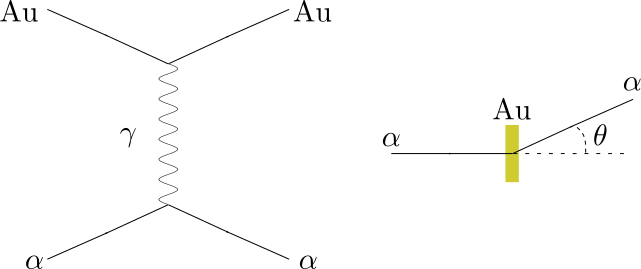
\includegraphics[scale=0.95]{scattering} %noinstiki
  \caption{Dispersi\'on de part\'\i culas $\alpha$ a trav\'es de una l\'amina de oro} %noinstiki
  \label{fig:sr} %noinstiki
\end{figure} %noinstiki<div id="fig:sr">Figura: Dispersi\'on</div>
%noinstiki![scattering](http://gfif.udea.edu.co/figfs/scattering.png)
%noinstiki

 
En general tendremos
\begin{equation}
\text{propagador:}\qquad \frac{1}{k^2-m^2},
\end{equation}
donde $k=(k_0,\mathbf{k})$




\section{Campos escalares complejos}
\label{sec:camp-escal-compl}
%to_en: \textsl{Some interesting physics emerges if we consider a system of two real scalar fields, $\phi_1$ and $\phi_2$, having the same mass $m$}. Then
En la secci\'on anterior se trabajo con un campo escalar real que s\'olo podr\'\i a describir un pion neutro. Para describir piones cargados debemos construir un campo escalar complejo. En mec\'anica cu\'antica la funci\'on de onda compleja puede describir parcialmente a un electr\'on cargado. Sin embargo la funci\'on de onda del electr\'on tambi\'en debe ser generalizada para poder dar cuenta del esp\'\i n. Esto corresponde al funci\'on de onda de la ecuaci\'on de Dirac en la secci\'on \ref{sec:ecuacion-de-dirac}.

De hecho, algunas consecuencias f\'\i sicas interesantes surgen si consideramos un sistema de dos campos escalares reales, $\phi_1$ y $\phi_2$, que tengan la misma masa $m$. Entonces
\begin{align}
  \label{eq:cplx}
  \mathcal{L}=\frac{1}{2}[\partial^\mu\phi_1\partial_\mu\phi_1-\frac{1}{2}m^2\phi_1^2]+\frac{1}{2}[\partial^\mu\phi_2\partial_\mu\phi_2-\frac{1}{2}m^2\phi_2^2]
\end{align}                                                     
%to_en: If we define
Si definimos
\begin{align}
  \label{eq:cplx_trans}
    \phi=&\frac{\phi_1+i\phi_2}{\sqrt{2}}\qquad\text{then}\\
    \phi^*=&\frac{\phi_1-i\phi_2}{\sqrt{2}},\qquad\text{and}\\
    \sqrt{2}\phi=&(\phi_1+i\phi_2)\nonumber\\
    \sqrt{2}\phi^*=&(\phi_1-i\phi_2).\qquad\text{Therefore}\nonumber\\
    \sqrt{2}(\phi+\phi^*)=&2\phi_1\nonumber\\
    \sqrt{2}(\phi-\phi^*)=&2i\phi_2.\qquad\text{Then}\nonumber\\
    \phi_1=&\frac{\phi+\phi^*}{\sqrt{2}}\label{eq:phi1}\\
    \phi_2=&\frac{\phi-\phi^*}{\sqrt{2}i}\label{eq:phi2}. %noinstiki
\end{align}
%to_en:Replacing eqs.~(\ref{eq:phi1})
%to_en:and (\ref{eq:phi2}) %noinstiki
%to_en:in eq.~(\ref{eq:cplx}) we have
Reemplazando la ecuaciones ~(\ref{eq:phi1})
y (\ref{eq:phi2}) %noinstiki
en la ec.~(\ref{eq:cplx}), tenemos
\begin{align}
  \mathcal{L}=&\frac{1}{4}[\partial^\mu(\phi+\phi^*)\partial_\mu(\phi+\phi^*)-\frac{1}{2}m^2(\phi+\phi^*)^2]\nonumber\\
 & +i^2\frac{1}{4}[\partial^\mu(\phi-\phi^*)\partial_\mu(\phi-\phi^*)-\frac{1}{2}m^2(\phi-\phi^*)^2]\nonumber\\
 =&\frac{1}{4}[\partial^\mu\phi\partial_\mu\phi+\partial^\mu\phi^*\partial_\mu\phi^*+2\partial^\mu\phi^*\partial_\mu\phi-m^2(\phi^2+{\phi^*}^2)+2\phi^*\phi]\nonumber\\
   &-\frac{1}{4}[\partial^\mu\phi\partial_\mu\phi+\partial^\mu\phi^*\partial_\mu\phi^*-2\partial^\mu\phi^*\partial_\mu\phi-m^2(\phi^2+{\phi^*}^2)-2\phi^*\phi]\nonumber\\
 =&\frac{1}{4}[4\partial^\mu\phi^*\partial_\mu\phi-4m^2\phi^*\phi]\nonumber\\
 \label{eq:41}
\mathcal{L}=&\partial^\mu\phi^*\partial_\mu\phi-m^2\phi^*\phi
\end{align}
%to_en:Generalizing eqs.~\eqref{eq:1} \eqref{eq:2} of section~\ref{sec:principio-de-minima-call},
%to_en:the corresponding expression for $\delta S=0$ is in this case~\ref{sec:principio-de-minima-call},
De la ec.~\eqref{eq:132} de la secci\'on~\ref{sec:principio-de-minima-call}, 

De las ecuaciones de Euler-Lagrange para $\phi^*$, usando el Lagrangiano en ec.~(\ref{eq:41})
\begin{align}
  \partial_\mu\left[
      \frac{\partial\mathcal{L}}{\partial(\partial_\mu\phi^*)}\right]-\frac{\partial\mathcal{L}}{\partial\phi^*}&=0\nonumber\\
    \partial_\mu\partial^\mu\phi+m^2\phi&=0\nonumber\\
    \label{eq:43}
    (\Box+m^2)\phi&=0,
\end{align}
y de la ecuaciones de Euler-Lagrange para $\phi$,
\begin{equation}
  \label{eq:44}
    (\Box+m^2)\phi^*=0.
\end{equation}
De este modo tanto $\phi$, como $\phi^*$, satisfacen la ecuaci\'on de Klein-Gordon. Cada campo adem\'as corresponde a una part\'\i cula de masa $m$ como en el caso de $\phi_1$ y $\phi_2$

%to_en:We now are interested in internal symmetries of the Lagrangian. Therefore we set $\delta x^\mu=0$, ($\Delta\phi=\delta\phi$). The conserved current can be defined as
Estamos ahora interesado en las simetr\'\i as internas del Lagrangiano. Entonces la corriente conservada puede definida en la secci\'on~\ref{sec:principio-de-minima-call}, eq.~\eqref{eq:jmuphi}
\begin{align}
  J^\mu=&\frac{\partial\mathcal{L}}{\partial(\partial_\mu\phi)}\delta\phi+\delta\phi^*\frac{\partial\mathcal{L}}{\partial(\partial_\mu\phi^*)}\nonumber\\
  \label{eq:45}
  J^\mu=&\partial^\mu\phi^*\delta\phi+\delta\phi^*\partial^\mu\phi.
\end{align}
Adem\'as de la invarianza de Lorentz, el Lagrangiano en ec,~(\ref{eq:41}) tambi\'en es invariante bajo el grupo de transformaciones U(1) definido en las secci\'on~\ref{sec:lagr-electr}, pero con una fase constante
\begin{equation*}
  U=e^{i\theta}\approx1+i\theta.
\end{equation*}
Entonces
\begin{align}
  \phi\overset{U}{\longrightarrow}\phi'&=e^{i\theta}\phi\approx(1+i\theta)\phi\nonumber\\
  &=\phi+i\theta\phi.
\end{align}
Entonces,
\begin{align}
  \delta\phi&=i\theta\phi\\
  \delta\phi^*&=-i\theta\phi^*.
\end{align}
Reemplazando en ec.~(\ref{eq:45})
\begin{equation}
\label{eq:46}
  J^\mu\propto -i\theta(\phi\partial^\mu\phi^*-\phi^*\partial^\mu\phi),
\end{equation}
y
\begin{equation}
\label{eq:47}
  \rho=J^0\propto-i\theta(\phi\frac{\partial\phi^*}{\partial t}-\phi^*\frac{\partial\phi}{\partial t}).
\end{equation}
Definimos $J^\mu$ como
\begin{equation}
  \label{eq:48}
   J^\mu= i(\phi^*\partial^\mu\phi-\phi\partial^\mu\phi^*),
\end{equation}
Como $\rho$ puede ser negativo no puede interpretarse como una
probalidad, como se hizo con la funci\'on de onda de la ecuaci\'on de
Scr\"odinger. Esto present\'o un obstaculo en la interpretaci\'on inicial de
la ecuaci\'on de Klein-Gordon. Sin embargo una vez se cuantiza el
campo escalar la probabilidad de los estados cu\'anticos queda bien
definida \cite{Gross}. 

Para interpretar a que corresponde la densidad de la ecuaci\'on de
Klein-Gordon para un campo escalar complejo considere la siguiente
soluci\'on a la ec.~(\ref{eq:43})
\begin{align}
  \phi&=\frac{1}{\sqrt{2\omega L^3}}
  \left[
    a\, e^{ik\cdot x}+b^*e^{-ik\cdot x}
  \right]\nonumber\\
  \label{eq:49}
   &=\frac{1}{\sqrt{2\omega L^3}}
   \left[
     a\, e^{i(wt-\mathbf{k}\cdot\mathbf{x})}+b^*e^{-i(wt-\mathbf{k}\cdot\mathbf{x})}
   \right]
\end{align}
Donde el factor global es una generalizaci\'on de la ec.~\eqref{eq:9} para el caso en 3 dimensiones. 

Usando la expresi\'on para $T^\mu_\nu$ se obtiene para el campo complejo
\begin{align}
  H&=\omega(a^*a+b^*b)\nonumber\\
  \mathbf{P}&=\mathbf{k}((a^*a+b^*b))
\end{align}

Sea
\begin{equation}
  \label{eq:50}
  \bar{\phi}=\frac{1}{\sqrt{2\omega L^3}}
  \left[
    a\, e^{i(\omega t-\mathbf{k}\cdot\mathbf{x})}-b^*e^{-i(\omega t-\mathbf{k}\cdot\mathbf{x})}
  \right]\,,
\end{equation}
entonces, 
\begin{align*}
 \frac{\partial \phi}{\partial t}=&i \omega \bar{\phi}\\
 \boldsymbol{\nabla}\phi=&-i \mathbf{k} \bar{\phi}\,,
\end{align*}
reemplazando en la ecuaci\'on (\ref{eq:43})
\begin{align}
\frac{\partial}{\partial t}\frac{\partial\phi}{\partial t}-\boldsymbol{\nabla}\cdot\boldsymbol{\nabla\phi}+m^2\phi&=0\nonumber\\
  iw\frac{\partial\bar{\phi}}{\partial t}+i\mathbf{k}\cdot\boldsymbol{\nabla}\bar{\phi}+m^2\phi&=0\nonumber\\
  (-w^2+\mathbf{k}^2+m^2)\phi&=0\nonumber\\
  (w^2-\mathbf{k}^2-m^2)\phi&=0.
\end{align}
Como era de esperarse, para que la ec.~(\ref{eq:49}) sea soluci\'on a la
ecuaci\'on de Klein-Gordon, $w$ y $\mathbf{k}$ deben satisfacer la
ecuaci\'on de energ\'\i a-momentum de la relatividad especial. 

La ec.~\eqref{eq:50} tambi\'en puede escribirse como
\begin{equation}
  \phi=a\,\phi^-+b^*\phi^+
\end{equation}
donde, 
\begin{align}
\label{eq:246}
  \phi^-&=\frac{1}{\sqrt{2\omega L^3}}e^{i(wt-\mathbf{k}\cdot\mathbf{x})}\nonumber\\
  \phi^+&=\frac{1}{\sqrt{2\omega L^3}}\, e^{-i(wt-\mathbf{k}\cdot\mathbf{x})}
\end{align}
son las soluciones de energ\'\i a negativa y positiva respectivamente, a la ecuaci\'on de Klein-Gordon, si
 $\omega$ es una cantidad definido positiva. Entonces, si $\theta\gt 0$
\begin{align}
  J^0_+&=i({\phi^+}^*\frac{\partial\phi^+}{\partial t}-\phi^+\frac{\partial{\phi^+}^*}{\partial t})\nonumber\\
  &=\frac{i}{2\omega L^3}[(-iw)-(iw)]\nonumber\\
  \label{eq:61}
  &=\frac{1}{L^3}\gt 0.
\end{align}
\begin{align}
  J^0_-&=-\frac{1}{L^3}\lt 0.
\end{align}
Note que el signo de la corriente s\'olo depende del signo de $\omega$. El signo de $\mathbf{k}$ establece en que direcci\'on se mueve la part\'\i cula.

Entonces, la carga conservada es
\begin{equation}
  Q^{\pm}=\int_Vd^3x\,J^0_{\pm}=\pm1
\end{equation}
Adem\'as de la expresi\'on para la energ\'\i a del campo en eq.~\eqref{eq:138}, y usando la ec.~\eqref{eq:45}.
\begin{align}
    T^\mu_\nu&=\frac{\partial\mathcal{L}}{\partial(\partial_\mu\phi)}(\partial_\nu\phi)+(\partial_\nu\phi^*)\frac{\partial\mathcal{L}}{\partial(\partial_\mu\phi^*)}
      -\delta^\mu_\nu\mathcal{L}  \nonumber\\
      &=\partial^\mu\phi^*\partial_\nu\phi+\partial_\nu\phi^*\partial^\mu\phi-\delta^\mu_\nu\mathcal{L}
\end{align}
\begin{align}
  T^0_0&=2\partial^0\phi\partial_0\phi^*-\partial^\mu\phi^*\partial_\mu\phi+m^2\phi^*\phi\nonumber\\
  &=\partial^0\phi\partial_0\phi^*-\partial^i\phi^*\partial_i\phi+m^2\phi^*\phi\nonumber\\
  &=\partial^0\phi\partial_0\phi^*+\boldsymbol{\nabla}\phi^*\cdot\boldsymbol{\nabla}\phi+m^2\phi^*\phi
\end{align}
\begin{align}
  T^i_0&=\partial^i\phi^*\partial_0\phi+\partial_0\phi^*\partial^i\phi
\end{align}
Para $\phi^+$ (o $\phi-$)
\begin{align}
  T^0_0&=\frac{1}{2\omega L^3}\left[(-i\omega)(i\omega)+(i\mathbf{k})\cdot(-i\mathbf{k})+m^2\right]\nonumber\\
 & =\frac{1}{2\omega L^3}\left[\omega^2+\mathbf{k}^2+m^2\right]\nonumber\\
& =\frac{1}{2\omega L^3}\left[\omega^2+\omega^2\right]\nonumber\\
& =\frac{\omega}{L^3}
\end{align}
y
\begin{equation}
  E^\pm=\int_Vd^3x\,T^0_0=\omega\gt 0
\end{equation}
Por consiguiente podemos interpretar $\phi^+$ como un campo representando
a una part\'\i cula de carga positiva (campo de frecuencia negativa) y a
$\phi^-$ como un campo representando a una part\'\i cula de carga negativa
(campo de frecuencia positiva). La cantidad conservada debido a la
invarianza de fase corresponde a la carga el\'ectrica. 

Un campo escalar real tendr\'\i a carga cero de acuerdo a la
ec (\ref{eq:47}).

Generalizando \eqref{eq:246} tenemos
\begin{align}
\label{eq:248}
\pi^+&\to,&  \phi^+_\to&=\frac{1}{\sqrt{2\omega L^3}}\, e^{i(-wt+\mathbf{k}\cdot\mathbf{x})}\nonumber\\
\pi^+&\gets,&  \phi^+_\gets&=\frac{1}{\sqrt{2\omega L^3}}\, e^{i(-wt-\mathbf{k}\cdot\mathbf{x})}\nonumber\\
\pi^-&\to,&    \phi^-_\to&=\frac{1}{\sqrt{2\omega L^3}}e^{i(+wt-\mathbf{k}\cdot\mathbf{x})}\nonumber\\
\pi^-&\gets,&    \phi^-_\gets&=\frac{1}{\sqrt{2\omega L^3}}e^{i(+wt+\mathbf{k}\cdot\mathbf{x})}
\end{align}
Para relacionar con el momentum de la part\'\i cula
\begin{align}
  \label{eq:42}
    T^0_i&=\frac{\partial\mathcal{L}}{\partial(\partial_0\phi)}(\partial_i\phi)+(\partial_i\phi^*)\frac{\partial\mathcal{L}}{\partial(\partial_0\phi^*)}\nonumber\\
&=\partial^0\phi^*\partial_i\phi+\partial_i\phi^*\partial^0\phi\,,
\end{align}
Tenemos para $\phi^\pm_\to=1/(\sqrt{2\omega L^3})\exp{[\mp i(\omega t-k^i x^i)]}$,   ${(\phi^\pm_\to)}^*=\phi^\mp_\to=1/(\sqrt{2\omega L^3})\exp{[\pm i(\omega t-k^i x^i)]}$
\begin{align}
T^0_i=&\partial^0\phi^\mp_\to\partial_i\phi^\pm_\to +\partial_i\phi^\mp_\to\partial^0\phi^\pm_\to \nonumber\\
=&\frac{1}{2\omega L^3}\left[(\pm i\omega)(\pm i k^i)+(\mp i k^i)(\mp i\omega)\right]\nonumber\\
  =&-\frac{k^i}{L^3}
\end{align}
Definimos
\begin{equation}
  P^i=-\int_Vd^3x\,T^0_i=k^i
\end{equation}
De modo que
\begin{align}
  \mathbf{P}=\mathbf{k}
\end{align}
Para las soluciones $\phi^{\pm}_\gets$, tenemos  $\mathbf{P}=-\mathbf{k}$. 

En el caso de una dimensi\'on $z$, el sentido de las flechas entonces representa la si la part\'\i cula se mueve a la derecha, $\to $ con $T^0_3<0$, o a la izquierda, $\gets$ $T^0_3>0$.


% \left(\right)


Si los campos escalares representan piones el campo escalar real puede
representar a un $\pi^0$, mientras que el campo escalar complejo junto
con su conjugado representar\'\i an al $\pi^+$ y al $\pi^-$. Tenemos dos casos
interesantes
\begin{enumerate} %noinstiki
%noinstiki
\item Para distancias suficientemente grandes entre piones cargados, las
interacciones nucleares ser\'\i an despreciables y solo interactuan
electromagn\'eticamente a trav\'es del intercambio de fotones. En este
caso los piones cargados ser\'\i an la fuente de la corriente
electromagn\'etica dada en la ec.~(\ref{eq:48}). El an\'alisis de este
caso dar\'a lugar a una Teor\'\i a Gauge Local Abelina, representada por el
grupo U(1).
\label{item:1} %noinstiki

\item A nivel de las interacciones nucleares, los tres piones ser\'\i an
indistinguibles y formarian un triplete de isospin fuerte que media la
interacci\'on, mientras que el neutr\'on y el prot\'on formar\'\i an un doblete
y ser\'\i an la fuente de los piones. Esto complementa el modelo de Yukawa presentado en la secci\'on~\ref{sec:ecuacion-de-klein} que requer\'\i a la existencia de tres piones para mediar la interacci\'on, el $\pi^\pm$ y $\pi^0$.  El an\'alisis de este
caso dar\'a lugar a una Teor\'\i a Gauge Local No Abelina, representada por el
grupo SU(2) y que conserva la carga de isosp\'\i n fuerte localmente.
\label{item:2} %noinstiki

\end{enumerate} %noinstiki

\section{Invarianza gauge local abeliana}
\label{sec:invar-gauge-local}
Considere la representaci\'on del Grupo U(1), que de acuerdo a la secci\'on~\ref{sec:lagr-electr} es
\begin{equation}
  U(x)=e^{i\theta(x)}
\end{equation}
En el Lagrangiano en ec.~(\ref{eq:41})
\begin{equation}
  \mathcal{L}=\left(\partial^\mu\phi\right)^*\partial_\mu\phi-m^2\phi^*\phi,
\end{equation}
el t\'ermino de masa es invariante bajo la transformaci\'on
\begin{align}
\phi\overset{U}{\to}\phi'&=U\phi\nonumber\\
\label{eq:51}
\phi^*\overset{U}{\to}{\phi^*}'&=\phi U^{-1},
\end{align}
pero el t\'ermino cin\'etico no lo es. Sin embargo, si cambiamos $\partial_\mu$, por una derivada covariante $\mathcal{D}_\mu$, tal que la derivada covariante del campo transforme como el campo:
\begin{align}
\mathcal{D}^\mu\phi\overset{U}{\to}\left(\mathcal{D}^\mu\phi\right)'&=U\left(\mathcal{D}^\mu\phi\right)\nonumber\\
\label{eq:52}
\left(\mathcal{D}^\mu\phi\right)^*\overset{U}{\to}{\left(\mathcal{D}^\mu\phi\right)^*\,}'&=\left(\mathcal{D}^\mu\phi\right)^*U^{-1},
\end{align}
entonces el Lagrangiano obtenido por reemplazo $\partial^\mu\to\mathcal{D}^\mu$:
\begin{equation}
  \label{eq:53}
  \mathcal{L}=\left(\mathcal{D}^\mu\phi\right)^*\mathcal{D}^\mu\phi-m^2\phi^*\phi,
\end{equation}
es invariante bajo el grupo de Transformaciones U(1): $\mathcal{L}\to\mathcal{L}'=\mathcal{L}$. Diremos en ese caso que el Lagrangiano, y por consiguiente la Acci\'on, es \emph{invariante gauge local} bajo U(1). 

Desarrollando la ec.~(\ref{eq:52}), tenemos que
\begin{align}
  \label{eq:247}
  \widehat{\mathcal{D}}_\mu\phi\to{\left(\widehat{\mathcal{D}}_\mu\phi\right)}'=
  {{\widehat{\mathcal{D}}}'}_\mu U\phi=U\widehat{\mathcal{D}}_\mu\phi
\end{align}
Cuando sea necesario indicaremos el caracter de operador de $\mathcal{D}$ con $\widehat{\mathcal{D}}$.

Por consiguiente
\begin{equation}
  {\mathcal{D}'}^\mu U=U\mathcal{D}^\mu
\end{equation}
\begin{equation}
  \label{eq:54}
  \mathcal{D}^\mu\to\left(
    \mathcal{D}^\mu
  \right)'=U\mathcal{D}^\mu U^{-1}
\end{equation}


Las ecs. (\ref{eq:52}) no se satisfacen para $\mathcal{D}^\mu=\partial^\mu$. Sin embargo, definiendo
\begin{equation}
  \label{eq:55}
\mathcal{D}^\mu=\partial^\mu-igA^\mu
\end{equation}
Para que las ecs. (\ref{eq:52}) se satisfagan, tenemo de la ecuaci\'on \eqref{eq:247} que
\begin{align}
  \label{eq:251}
   {\mathcal{D}}^\mu\phi\to{\left({\mathcal{D}}^\mu\phi\right)}'=
  (\partial^\mu-i g {A'}^\mu) U\phi=&U(\partial^\mu-i g {A}^\mu\mathcal{D})\phi\nonumber\\
  U\partial^\mu\phi+(\partial^\mu U)\phi-i g {A'}^\mu U \phi=&U\partial^\mu\phi-i g {A}^\mu \phi\nonumber\\
  (\partial^\mu U)\phi-i g {A'}^\mu U \phi=&-i g U {A}^\mu \phi\nonumber\\
  -i g {A'}^\mu U \phi=&-(\partial^\mu U)\phi-i g U {A}^\mu \phi\nonumber\\
   {A'}^\mu U =&\frac{1}{i g}(\partial^\mu U)+ U{A}^\mu \nonumber\\
   {A'}^\mu  =&-\frac{i}{g}(\partial^\mu U)U^{-1}+ U{A}^\mu U^{-1}\,.
\end{align}
From this general formula we have

\begin{align}
  A^\mu\overset{U}{\to}{A^\mu}'&=UA^\mu U^{-1}-\frac{i}{g}(\partial^\mu U)U^{-1}\nonumber\\
  &=A^\mu-\frac{i}{g}(\partial^\mu U)U^{-1}\nonumber\\
  &=A^\mu-\frac{i}{g}\left(i\partial^\mu\theta\right)UU^{-1}\nonumber\\
  \label{eq:159}
  &= A^\mu+\frac{1}{g}\partial^\mu\theta\,.
\end{align}
As\'\i, el campo $A^\mu$ que se requiere para satisfacer las propiedades de la derivada covariante transforma justamente como el campo vectorial electromagn\'etico. La ec.~(\ref{eq:55}) da lugar a la \emph{sustituci\'on m\'\i nima} del operador de momentum
\begin{equation}
  p^\mu\to p^\mu+gA^\mu
\end{equation}

Veremos que la carga conservada $U(1)$ se puede identificar con la carga el\'ectrica. Entonces fijamos
\begin{equation}
  g=-e
\end{equation}


Podemos encontrar que
\begin{align}
  \label{eq:67}
  \widehat{F}^{\mu\nu}&=\frac{i}{g}[\mathcal{D}^\mu,\mathcal{D}^\nu]
\end{align}
ya que
\begin{align}
  \label{eq:164}
   \widehat{F}^{\mu\nu}\phi =&\frac{i}{g}[\partial^\mu-igA^\mu,\partial^\nu-igA^\nu]\phi\nonumber\\
  =&\frac{i}{g}\left[\left(\partial^\mu-igA^\mu\right)\left(\partial^\nu-igA^\nu\right)\phi
    -\left(\partial^\nu-igA^\nu\right)\left(\partial^\mu-igA^\mu\right)\phi\right]\nonumber\\
  =&\frac{i}{g}\left\{\partial^\mu\partial^\nu\phi-g^2A^\mu A^\nu\phi-ig[\partial^\mu(A^\nu\phi)+A^\mu\partial^\nu\phi]
    -\partial^\nu\partial^\mu\phi+g^2A^\nu A^\mu\phi+ig[\partial^\nu(A^\mu\phi)+A^\nu\partial^\mu\phi]\right\}\nonumber\\
  =&\frac{i}{g}\{(\partial^\mu\partial^\nu-\partial^\nu\partial^\mu)\phi-g^2(A^\mu A^\nu-A^\nu A^\mu)\phi
  -ig[(\partial^\mu A^\nu)-(\partial^\nu A^\mu)]\phi\nonumber\\
  &-ig[A^\nu\partial^\mu\phi+A^\mu\partial^\nu\phi-A^\mu\partial^\nu\phi+A^\nu\partial^\mu\phi]\}\nonumber\\
=&[(\partial^\mu A^\nu)-(\partial^\nu A^\mu)-ig(A^\mu A^\nu-A^\nu A^\mu)]\phi
\end{align}
Como $A^\mu$ y $A^\nu$ conmutan
\begin{align}
   F^{\mu\nu}&=\partial^\mu A^\nu-\partial^\nu A^\mu
\end{align}

Con esta expresi\'on para $\widehat{F}^{\mu\nu}$ podemos demostrar su invarianza gauge a partir de la transformaci\'on de la derivada covariante
\begin{align}
  \label{eq:68}
  \left(
    \widehat{F}^{\mu\nu}
  \right)'&=\frac{i}{g}\left[{\mathcal{D}'}^\mu,{\mathcal{D}'}^\nu\right]\nonumber\\
&=\frac{i}{g}\left[U{\mathcal{D}}^\mu U^{-1},U{\mathcal{D}}^\nu U^{-1}\right]\nonumber\\
&=U\widehat{F}^{\mu\nu}U^{-1}\nonumber\\
  &=\widehat{F}^{\mu\nu}\,.
\end{align}

El Lagrangiano m\'as general es, que incluye todos los t\'erminos invariantes gauge y renormalizables para los campos $\phi$ y $A^\mu$ es
\begin{equation}
  \label{eq:56}
  \mathcal{L}=\left(\mathcal{D}^\mu\phi\right)^*\mathcal{D}_\mu\phi-m^2\phi^*\phi-\frac{1}{4}F^{\mu\nu}F_{\mu\nu}\,.
\end{equation}
Desarrollando el primer t\'ermino
\begin{align}
  \left(\mathcal{D}^\mu\phi\right)^*\mathcal{D}_\mu\phi=&\left[\left(\partial^\mu+ieA^\mu\right)\phi\right]^*\left(\partial_\mu+ieA_\mu\right)\phi\nonumber\\  
  =&\left(\partial^\mu\phi^*-ieA^\mu\phi^*\right)\left(\partial_\mu\phi+ieA_\mu\phi\right)\nonumber\\
  =&\partial^\mu\phi^*\partial_\mu\phi+ieA_\mu(\partial^\mu\phi^*)\phi-ieA^\mu\phi^*\partial_\mu\phi+e^2A^\mu A_\mu\phi^*\phi
\end{align}
Por consiguiente el Lagrangiano en ec.~\eqref{eq:56} puede escribirse como
\begin{equation}
  \label{eq:250}
  \mathcal{L}=\mathcal{L}_{\text{escalar}}-\frac{1}{4}F^{\mu\nu}F_{\mu\nu}+\mathcal{L}_{int}
\end{equation}
donde
\begin{align}
  \label{eq:73}
  \mathcal{L}_{\text{int}}&=-ieA_\mu(\phi^*\partial^\mu\phi-\phi\partial^\mu\phi^*)+e^2A^\mu A_\mu\phi^*\phi\,.
\end{align}
El campo vectorial $A^\mu$ aparece como consecuencia de la invarianza gauge del Lagrangiano en ec.~\eqref{eq:53}. En tal caso lo llamaremos un \emph{bos\'on gauge}. 

De las ecuaciones de Euler-Lagrange tenemos
\begin{align}
    \partial_\mu\left[
    \frac{\partial\mathcal{L}}{\partial(\partial_\mu A_\nu)}  
  \right]-\frac{\partial\mathcal{L}}{\partial A_\nu}&=0\nonumber\\
-\partial_\mu F^{\mu\nu}-e\left[-i(\phi^*\partial^\nu\phi-\phi\partial^\nu\phi^*)+2eA^\nu \phi^*\phi\right]=0\,.
\end{align}
%\left(\right)
Las ecuaciones de movimiento para el campo vectorial son entonces
\begin{equation}
  \partial_\mu F^{\mu\nu}=ej^\nu
\end{equation}
donde 
\begin{equation}
\label{eq:60}
  j^\mu=i
  \left[
    \phi^*\partial^\mu\phi-
      (\partial^\mu\phi^*)\phi
  \right]-2e\,A^\mu\phi^*\phi=J^\mu-2e\,A^\mu\phi^*\phi\,.
\end{equation}
Usando la primera ecuaci\'on en (\ref{eq:45}), tenemos que ($\mathcal{D}^\mu=\partial^\mu+ie\,A^\mu$)
\begin{equation}
  j^\mu=i
  \left[
    \phi^*\mathcal{D}^\mu\phi-
    \left(
      \mathcal{D}^\mu\phi
    \right)^*\phi
  \right].
\end{equation}
De otro lado, las ecuaciones de movimiento para el campo escalar complejo 
\begin{align}
  \label{eq:155}
    \partial_\mu\left[
      \frac{\partial\mathcal{L}}{\partial(\partial_\mu\phi^*)}\right]-\frac{\partial\mathcal{L}}{\partial\phi^*}&=0\nonumber\\
    \partial_\mu(\partial^\mu\phi+i e A^\mu\phi)-(-m^2\phi-ieA_\mu\partial^\mu\phi+e^2A^\mu A_\mu\phi)&=0\nonumber\\
   \partial_\mu\partial^\mu\phi+m^2\phi+ie\partial_\mu (A^\mu\phi)+ieA^\mu\partial_\mu\phi-e^2A^\mu A_\mu\phi&=0
\end{align}
dan lugar a
\begin{equation}
  (\Box +m^2+\hat{U}(x))\phi=0,
\end{equation}
donde
\begin{equation}
  \label{eq:58}
  \hat{U}(x)=ie(A^\mu\partial_\mu+\partial_\mu A^\mu)-e^2A^\mu A_\mu
\end{equation}
El operado en el segundo t\'ermino opera en $A_\mu$ y $\phi$. A la luz de los resultados la escogencia de la derivada covariante en la ec.~\eqref{eq:55}, puede justificarse adicionalmente a partir de la Fuerza de Lorentz para una part\'\i cula de carga $q$  moviendose con una velocidad $v$ bajo la influencia tanto del campo magn\'etico como del campo el\'ectrico
\begin{equation}
  \mathbf{F}=q\mathbf{E}+q\mathbf{v}\times\mathbf{B}.
\end{equation}
Esta expresi\'on puede ser deriva, a trav\'es de las ecuaciones de Hamilton, del Hamiltoniano cl\'asico
\begin{align}
  \label{eq:158}
  H&=\frac{1}{2m}(\mathbf{p}-q\mathbf{A})^2+qA_0\\
  H-qA^0&=\frac{1}{2m}(\mathbf{p}-q\mathbf{A})^2\nonumber
\end{align}
que a su vez puede obtenerse del Hamiltoniano para una part\'\i cula libre con el reemplazo
\begin{align}
  H&\to H-qA^0& \mathbf{p}\to\mathbf{p}-q\mathbf{A}
\end{align}
En t\'erminos de los operadores $\hat H$ y $\hat{\mathbf{p}}$, tenemos
\begin{align}
  i\frac{\partial}{\partial t}&\to i\frac{\partial}{\partial t}-qA^0&  -i\nabla&\to-i\nabla-q\mathbf{A}\nonumber\\ 
  \frac{\partial}{\partial t}&\to\frac{\partial}{\partial t}+iqA^0&  \partial_i&\to\partial_i-iqA^i=\partial_i+iqA_i\,.
\end{align}
De modo que
\begin{equation}
  \partial^\mu=(\partial^00,\partial^i)\to\mathcal{D}^\mu=(\partial^0+iqA^0,\partial^i+iqA^i)=\partial^\mu+iqA^\mu\,.
\end{equation}


\subsection{Aplicaci\'on a barrera de potencial}

Considere una barrera de potencial,
\begin{equation}
  A^0=\begin{cases}
    0&\text{A la izquierda de la barrera (Regi\'on I)}\\
    V&\text{A la derecha de la barrera (Regi\'on II)}
  \end{cases}
\end{equation} 
tal como se muestra en la figura~\ref{fig:barrier}.
Las componentes del campo vectorial son $\mathbf{A}=0$ y $A_0=V$, con $A_0$ independiente del tiempo pues el potencial es constante. Entonces, de la ec.~(\ref{eq:58}) tenemos que para le Regi\'on II
\begin{align}
  \hat{U}(x)&=ie(A^0\partial_0+\partial_0 A^0)-e^2A_0^2\nonumber\\
  &=ie(A^0\partial_0+A^0\partial_0 )-e^2A_0^2\nonumber\\
&=2ieV\frac{\partial}{\partial t}-e^2V^2
\end{align}
y
\begin{equation}
  \label{eq:59}
  (\Box +m^2+2ieV\frac{\partial}{\partial t}-e^2V^2)\phi=0\,.
\end{equation}
Se sugiere que en la Regi\'on I
\begin{equation}
  \phi_{\text{I}}=A\,e^{i(pz-Et)}+B\,e^{-i(pz+Et)}
\end{equation}
De acuerdo al c\'alculo de la corriente en ec.~\eqref{eq:61} esta soluci\'on representa part\'\i culas con carga positiva. Adem\'as de la ec.\eqref{eq:248} la soluci\'on con coeficiente $A$ representa un $\pi^+$ moviendose a la derecha, mientras que la de coeficiente $B$ representa un $\pi^+$ moviendose a la izquierda.

Otra forma de mostrar con que direcci\'on las soluciones evolucionan con el tiempo es haciendo paquetes de onda \cite{Gross}. El paquete de onda es
\begin{align}
  \label{eq:156}
  e^{i(pz-Et)}&=\exp\left[i\left(\sqrt{E^2-m^2}z-Et\right)\right]\nonumber\\
  &\to\int_{E_0-\Delta E}^{E_0+\Delta E}dE\;\exp\left[i\left(\sqrt{E^2-m^2}z-Et\right)\right]
\end{align}
sea $u=E-E_0\ll1$, entonces $E=u+E_0$, $dE=du$, $E=E_0-\Delta E$ da lugar a $u=-\Delta E$, y
\begin{align}
  \sqrt{E^2-m^2}&=\sqrt{(u+E_0)^2-m^2}=\sqrt{u^2+2uE_0+E_0^2-m^2}\approx\sqrt{2uE_0+p_0^2}\nonumber\\
  &=p_0\sqrt{1+\frac{2uE_0}{p_0^2}}\approx p_0(1+\frac{uE_0}{p_0^2})=p_0+\frac{uE_0}{p_0}
\end{align}
donde $p_0^2\equiv|\mathbf{p}_0|^2=E_0^2-m^2$. Para una part\'\i cula no relativista $E_0/p_0=m/(mv_0)=1/v_0$. En general
\begin{align}
  v_0=\frac{p_0}{E_0}
\end{align}
\begin{equation}
  \sqrt{E^2-m^2}\approx p_0+\frac{u}{v_0}
\end{equation}
sustituyendo en ec.~\eqref{eq:156}
\begin{align}
  e^{i(pz-Et)}&\to\int_{-\Delta E}^{\Delta E}du\;\exp\left\{i\left[\left(p_0+\frac{u}{v_0}\right)z-(u+E_0)t\right]\right\}
\end{align}
\begin{align}
  &\to e^{ip_0z-E_0t}\int_{-\Delta E}^{\Delta E}du\;\exp\left[i\left(\frac{u}{v_0}z-ut\right)\right]\nonumber\\
\end{align}
\begin{align}
    &\to e^{ip_0z-E_0t}\int_{-\Delta E}^{\Delta E}du\;\exp\left[iu\left(\frac{z}{v_0}-t\right)\right]\nonumber\\
\end{align}
\begin{align}
    &\to e^{ip_0z-E_0t}\int_{-\Delta E}^{\Delta E}du\;\exp\left[iu\left(\frac{z-v_0t}{v_0}\right)\right]\nonumber\\
\end{align}
Que corresponde a un pulso de energ\'\i a $E_0$ y momentum $p_0$ movi\'endose hacia la derecha
Sea
\begin{equation}
  \eta^-=\frac{z-v_0t}{v_0}
\end{equation}
Entonces
\begin{equation}
  f(\eta)=\int_{-\Delta E}^{\Delta E}dE\,e^{iE\eta}=2\frac{\sin(\eta\Delta E)}{\eta}
\end{equation}


%\left(\right)
\begin{equation}
  \varphi_I = A\,e^{i(p_0z-E_0t)}f\left(\frac{z-v_0t}{v_0}\right)+B\,e^{-i(p_0z+E_0t)}f\left(\frac{z+v_0t}{v_0}\right),
\end{equation}
y $v_0=p_0/E_0$. Entonces, la parte con coeficiente $A$ corresponde a un $\pi^+$ incidente moviendose hacia la derecha, y la parte con coeficiente $B$ a un $\pi^+$ reflejado moviendose hacia la izquierda (ver figura \ref{fig:barrier} ).
%noinstiki
\begin{figure} %noinstiki 
  \centering %noinstiki
  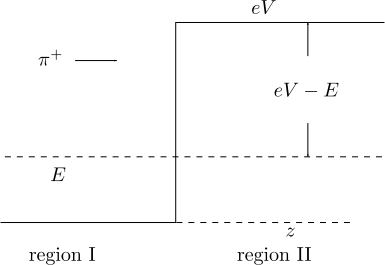
\includegraphics{barrier} %noinstiki
  \caption{Barrera de potencial} %noinstiki
  \label{fig:barrier} %noinstiki
\end{figure}  %noinstiki<div id="fig:barrier">Figura: Barrera de Potencial</div>
%noinstiki![barrier](http://gfif.udea.edu.co/figfs/barrier.png)
%noinstiki

Para la Regi\'on II, consideramos exponenciales de la misma fase que en la regi\'on I pero  con el momentum modificado debido ala presencia del potencial. En la regi\'on I las soluciones correspond\'\i an a part\'\i culas con $J^0=J^0_+\gt 0$. En la regi\'on II deberemos calcular los correspondientes $j^0$ de la ec.~\eqref{eq:60} e interpretar el signo resultante
\begin{equation}
  \label{eq:249}
  \phi_{II}=C\,e^{i(-Pz-Et)}+D\,e^{i(Pz-Et)}.
\end{equation}
Esta es soluci\'on a la ec.~\eqref{eq:59}
\begin{align}
  \left(\frac{\partial^2}{\partial t^2}-\frac{\partial^2}{\partial z^2}+m^2+2ieV\frac{\partial}{\partial t}-e^2V^2\right)\phi_{II}&=0\nonumber\\
  \left(-E^2+P^2+m^2+2eVE-e^2V^2\right)\phi_{II}&=0\nonumber\\
  \left[-(eV-E)^2+P^2+m^2\right]\phi_{II}&=0
\end{align}
de modo que

\begin{equation}
  P=\sqrt{(eV-E)^2-m^2}
\end{equation}
Note que $P\to p$ cuando $V=0$. Si $eV-E\lt m$ tenemos la soluci\'on amortiguada convencional. Sin embargo, en el caso de una barrera alta $eV-E\gt m$ tendremos soluciones oscilatorias. En adelante nos concentraremos en \'esta posibilidad, que corresponde a una barrera suficientemente alta.

El c\'alculo de la corriente en la Regi\'on II, esta dado por $j^\mu$ en la ec.~\eqref{eq:60}. Para $C=0$ o $D=0$,
\begin{align}
  Q=\int_0^L j^0dz&=\int_0^L\left\{i\left[\phi^*\partial^0\phi-\left(\partial^0\phi^*\right)\phi\right]-2e\,A^0\phi^*\phi\right\}dz\nonumber\\
&=\int_0^L\left\{i[-iE-(iE)]-2eV\right\}|\phi|^2\,dz\nonumber\\
&=\begin{cases}
  -2|C|^2\int_0^L (eV-E)\,dz=-2|C|^2 L (eV-E)\lt 0, & D=0\\
-2|D|^2\int_0^L (eV-E)\,dz=-2|D|^2 L (eV-E)\lt 0, & C=0
\end{cases}
\end{align}
%\left(\right)
y corresponde a una part\'\i cula cargada negativamente que interpretaremos como un $\pi^-$. Para identificar cual es el transmitido, es decir moviendose hacia la derecha usaremos de nuevo los dos m\'etodos descritos anteriormente. De la expresi\'on para el momentum tenemos
\begin{align}
  T^0_3=\frac{\partial\mathcal{L}}{\partial(\partial_0\phi)}\partial_3\phi+\partial_3\phi^*\frac{\partial\mathcal{L}}{\partial(\partial_0\phi^*)}\,,
\end{align}
donde el Lagrangiano obtenido a partir de la ec.~(\ref{eq:250}) es
\begin{align}
  \mathcal{L}=\partial^\mu\phi^*\partial_\mu\phi-m^2\phi^*\phi-\frac{1}{4}F^{\mu\nu}F_{\mu\nu}-i e V(\phi^*\partial_0\phi-\phi\partial_0\phi^*)+e^2{V}^2\phi^*\phi\,.
\end{align}
Entonces
\begin{align}
  T^0_3=&(\partial^0\phi^*-i e V\phi^*)\partial_3\phi+\partial_3\phi^*(\partial^0\phi+i e V\phi)\,.
\end{align}
De la ec. \eqref{eq:249}, para $\phi\propto e^{i(\mp P z-E t)}$, tenemos
\begin{align}
  T^0_3\propto&[i E-i e V](\mp i P)+(\pm i P)[-i E+i e V]\nonumber\\
  \propto&-2\times(\mp1)(E- e V)P\nonumber\\
  \propto&
  \begin{cases}
    -2(e V-E)P&D=0\\
    +2(e V-E)P&C=0\,.
  \end{cases}
\end{align}
Para una la barrera alta $eV-E>m>0$, de acuerdo a las convenciones, si $T^0_3<0$ la part\'\i cula se mueve hacia la derecha, y se mueve a la izquierda si $T^0_3>0$. De modo que la soluci\'on con coeficiente $C$ cooresponde a un $\pi^-$ moviendose a la derecha y la soluci\'on con coefciente $D$ corresponde a un $\pi^-$ moviendose a la izquierda. 
Note que cuando $V=0$, la soluci\'on $C e^{i(-P z-E t)}$,  $j^0>0$ y $T^0_3>0$ corresponde a $\pi^+$ moviendose a la izquierda. Para completar la descripci\'on, consideramos un $\pi^+$ moviendose a la derecha hacia la barrera como en la figura \ref{fig:barrier}. Esto significa que cualquier mes\'on $\pi^-$ debe ser producido por la interacci\'on con la barrera y viajar\'a hacia la derecha dentro de la regi\'on II. De aqu\'\i{} que para la condici\'on de frontera $D=0$, la soluci\'on  es
\begin{align}
   \phi_{\text{I}}=&A\,e^{i(pz-Et)}+B\,e^{-i(pz+Et)}\nonumber\\
   \phi_{II}=&C\,e^{i(-Pz-Et)}.
\end{align}
 
De otro lado podemos  construir el paquete de onda correspondiente en cada caso. Por ejemplo la condici\'on de frontera $D=0$  da lugar  a una part\'\i cula $\pi^-$ movi\'endose a la derecha. En efecto, el paquete de onda es
\begin{equation}
  \varphi_{II}=C\,e^{-i(P_0z+E_0t)}f\left(\frac{z-u_0t}{u_0}\right),
\end{equation}
con
\begin{equation}
  u_0=\frac{P_0}{eV-E_0}=\frac{P_0}{\sqrt{P_0^2+m^2}}
\end{equation}
Note que en el caso $V=0$, esta da lugar a un $\pi^+$ moviendose a la izquierda como era de esperarse. De manera que emerge un marco consistente de un part\'\i cula de masa $m$ y carga $-e$ moviendose hac\'\i a la derecha.  De aqu\'\i{} que para la condici\'on de frontera $D=0$, la soluci\'on normalizando $A=1$ es \cite{Gross}
\begin{align}
  \phi_I&=e^{i(p_0z-E_0t)}f\left(\frac{z-v_0t}{v_0}\right)
  -\frac{P_0+p_0}{P_0-p_0}\,e^{-i(p_0z+E_0t)}f\left(\frac{z+v_0t}{v_0}\right),\nonumber\\
  \phi_{II}&=-\frac{2p_0}{P_0-p_0}e^{-i(P_0z+E_0t)}f\left(\frac{z-u_0t}{u_0}\right),
\end{align}
Este resultado se interpreta diciendo que el pi\'on incidente no solo se dispersa en la barrera ($B\neq1$), sino que tambi\'en estimula la barrera para producir un par $\pi^+\pi^-$, el $\pi-$ viaja dentro de la barrera la cual ve como un hueco, mientras que el $\pi^+$ producido por la barrera viaja hacia la izquierda. Si $J^0$ y $j^0$ son interpretados como la densidad de carga, la interpretaci\'on es consistente y tiene sentido f\'\i sico. La energ\'\i a y la carga se conservan \cite{Gross}. 


\begin{example} %noinstiki **Ejemplo**
Escriba la ec.~\eqref{eq:56} en coordenadas polares.

Sea $\phi=e^{i\eta(x)}\rho(x)/\sqrt{2}$, con $\eta$ y $\rho$ reales. Bajo una tranformaci\'on gauge
\begin{align}
A^\mu\to {A'}^\mu&=A^\mu+\frac{1}{g}\partial^\mu\theta\nonumber\\
  \label{eq:86}
  \phi\to\phi'&=e^{i\theta(x)}e^{i\eta(x)}\frac{\rho(x)}{\sqrt{2}}
\end{align}
Si fijamos el gauge tal que $\theta=-\eta$, entonces $\phi'=\rho$, y
% WARNING change rho by rho/sqrt(2)
% \begin{equation}
%     F^{\mu\nu}F_{\mu\nu}&\to\left(F^{\mu\nu}F_{\mu\nu} \right)'=F^{\mu\nu}F_{\mu\nu}\nonumber\\
% \end{equation}
% \begin{align}
%   \mathcal{L}\to\mathcal{L}'=&\left[\left(\mathcal{D}_\mu\right)'\phi'\right]^*\left(\mathcal{D}^\mu\right)'\phi'-\left(m^2\phi^*\phi\right)'-\frac{1}{4}F^{\mu\nu}F_{\mu\nu}\nonumber\\
%   \mathcal{L}\to\mathcal{L}'=&\left[\left(\mathcal{D}_\mu\right)'\phi'\right]^*U\mathcal{D}^\mu\left(U^{-1}\phi'\right)-\left(m^2\phi^*\phi\right)'-\frac{1}{4}F^{\mu\nu}F_{\mu\nu}\nonumber\\
% =&\left[\left(U\partial_\mu U^{-1}\right)\phi'+UU^{-1}\partial_\mu\phi'-igUA_\mu U^{-1}\phi'\right]^*\left[\left(U\partial^\mu U^{-1}\right)\phi'+UU^{-1}\partial^\mu\phi'-igUA^\mu U^{-1}\phi'\right]\nonumber\\
% &-\left(m^2\phi^*\phi\right)'-\frac{1}{4}F^{\mu\nu}F_{\mu\nu}\nonumber\\
% =&\left[-i\left(\partial_\mu\eta\right){\phi^*}'+\partial_\mu{\phi^*}'+igA_\mu{\phi^*}'\right]\left[i\left(\partial^\mu\eta\right)\phi'+\partial^\mu\phi'-igA^\mu\phi'\right]\nonumber\\
% &-\left(m^2\phi^*\phi\right)'-\frac{1}{4}F^{\mu\nu}F_{\mu\nu}\nonumber\\
% =&\left\{\partial_\mu{\phi^*}'-i\left[\left(\partial_\mu\eta\right){\phi^*}'-gA_\mu{\phi^*}'\right]\right\}\left\{\partial^\mu\phi'+i\left[\left(\partial^\mu\eta\right)\phi'-gA^\mu\phi'\right]\right\}\nonumber\\
% &-\left(m^2\phi^*\phi\right)'-\frac{1}{4}F^{\mu\nu}F_{\mu\nu}\nonumber\\
% =&\left\{\partial_\mu\rho-i\left[\left(\partial_\mu\eta\right)-gA_\mu\right]\rho\right\}\left\{\partial^\mu\rho+i\left[\left(\partial^\mu\eta\right)-gA^\mu\right]\rho\right\}\nonumber\\
% &-m^2\rho^2-\frac{1}{4}F^{\mu\nu}F_{\mu\nu}\nonumber\\
% =& \partial_\mu\rho\partial^\mu\rho-m^2\rho^2+\left[\left(\partial_\mu\eta\right)-gA_\mu\right]\left[\left(\partial^\mu\eta\right)-gA^\mu\right]\rho\rho-\frac{1}{4}F^{\mu\nu}F_{\mu\nu}\nonumber\\
% =& \partial_\mu\rho\partial^\mu\rho-\tfrac{1}{2}\left(2m^2\right)\rho^2+ \partial_\mu\eta\partial^\mu\eta\rho\rho-2g\partial_\mu\eta A^\mu\rho\rho+g^2A_\mu A^\mu\rho\rho-\frac{1}{4}F^{\mu\nu}F_{\mu\nu}.
% \end{align}
% Entonces en este gauge, aparece una part\'\i cula escalar real con  el doble de  masa interacuando con otra part\'\i cula escalar sin masa y sin t\'ermino cin\'etico. 

\begin{align}
  \mathcal{L}\to\mathcal{L}'=&\left[\left(\mathcal{D}_\mu\right)'\phi'\right]^*\left(\mathcal{D}^\mu\right)'\phi'-\left(m^2\phi^*\phi\right)'-\frac{1}{4}\left(F^{\mu\nu}F_{\mu\nu}\right)'\nonumber\\
  \mathcal{L}\to\mathcal{L}'=&\left(\partial_\mu+ig{A_\mu}'\right){\phi^*}'\left(\partial^\mu-ig{A^\mu}'\right)\phi'-\left(m^2\phi^*\phi\right)'-\frac{1}{4}\left(F^{\mu\nu}F_{\mu\nu}\right)'\nonumber\\
=&\tfrac{1}{2}\left(\partial_\mu+ig{A_\mu}'\right)\rho\left(\partial^\mu-ig{A^\mu}'\right)\rho-\tfrac{1}{2}m^2\rho^2-\frac{1}{4}\left(F^{\mu\nu}F_{\mu\nu}\right)'\nonumber
\end{align}
En adelante, podemos quitar la prima del campo $A^\mu$
\begin{equation}
  \mathcal{L}=\tfrac{1}{2}\partial^\mu\rho\partial_\mu\rho-\tfrac{1}{2}m^2\rho+g^2A^\mu A_\mu\rho^2-\frac{1}{4}F^{\mu\nu}F_{\mu\nu}
\end{equation}

Aunque este gauge es de poca utilidad en este contexto, ser\'a de mucha utilidad en la discusi\'on del rompimiento espont\'aneo de simetr\'\i a.
\end{example} %noinstiki

\section{Aplicaci\'on a la mec\'anica cu\'antica}
\label{sec:aplic-la-mecan}
De la ecuaci\'on (\ref{eq:158}) podemos obtener la ecuaci\'on de Sch\"odinger en presencia de un campo electromagn\'etico
\begin{align}
    \widehat{H}\psi&=\left[\frac{1}{2m}(\hat{\mathbf{p}}-q\mathbf{A})^2+qA_0\right]\psi\nonumber\\
i\frac{\partial}{\partial t}\psi&=\left[\frac{1}{2m}(-i\mathbf{\nabla}-q\mathbf{A})^2+qA_0\right]\psi\,.
\end{align}
Que puede reescribirse como
\begin{align}
  i\left(\frac{\partial}{\partial t}+iqA^0\right)\psi&=i^2\frac{1}{2m}(\mathbf{\nabla}-iq\mathbf{A})^2\psi\nonumber\\
  i\left(\frac{\partial}{\partial t}+iqA^0\right)\psi&=-\frac{1}{2m}(\mathbf{\nabla}-iq\mathbf{A})^2\psi
\end{align}
Definiendo el cuadrivector
\begin{align}
  \mathcal{D}^\mu&=(\mathcal{D}^0,-\boldsymbol{\mathcal{D}})\nonumber\\
  &\equiv\left(\frac{\partial}{\partial t}+iqA^0,-(\mathbf{\nabla}-iq\mathbf{A})\right)\nonumber\\
  &=\left(\frac{\partial}{\partial t}+iqA^0,-\partial_i+iqA^i)\right)\nonumber\\
  &=\left(\frac{\partial}{\partial t}+iqA^0,\partial^i+iqA^i\right)\nonumber\\
  &=\partial^\mu+iqA^\mu
\end{align}
tenemos
\begin{equation}
  \label{eq:161}
  i\mathcal{D}^0\psi=-\frac{1}{2m}\boldsymbol{\mathcal{D}}^2\psi
\end{equation}
que para $A^\mu=0$ se reduce a la ecuaci\'on de Schr\"odinger para una part\'\i cula libre. 
Bajo la transformaci\'on gauge en el campo $A^\mu$ de la ec.~(\ref{eq:159}),
\begin{align}
  A^0\to {A'}^0&=A^0-\frac{1}{q}\partial^0\theta\nonumber\\
  \mathbf{A}\to \mathbf{A}'&=\mathbf{A}+\frac{1}{q}\boldsymbol{\nabla}\theta
\end{align}

 los campos $\mathbf{E}$ y $\mathbf{B}$ permanecen los mismos. Para que la mec\'anica cu\'antica sea consistente con las ecuaciones de Maxwell es necesario que las transformaciones gauge (\ref{eq:159}) de los potenciales de Maxwell est\'en acompa\~nados por una transformaci\'on de la funci\'on de onda, $\psi\to\psi'$, donde $\psi'$ satisface la ecuaci\'on
\begin{align}
  \label{eq:160}
   i{\mathcal{D}'}^0\psi'&=-\frac{1}{2m}{\boldsymbol{\mathcal{D}}'}^2\psi'\nonumber\\
 i\frac{\partial}{\partial t}\psi'&=\left[\frac{1}{2m}(-i\mathbf{\nabla}-q\mathbf{A}')^2+q{A'}_0\right]\psi'\,.
\end{align}
Como la forma de la ecuaci\'on (\ref{eq:160}) es exactamente la misma que la forma de (\ref{eq:161}) entonces ambas describen la misma f\'\i sica. Si podemos encontrar la forma de $\psi'$ podemos afirmar que la ec.~(\ref{eq:161}) es covariante gauge, lo que significa que mantiene la misma forma bajo una transformaci\'on gauge. Como conocemos como transforma $A^\mu$ podemos encontrar cual debe ser el $\psi'$ que hace que la ecuaci\'on (\ref{eq:160}) sea consistente con (\ref{eq:161}). Vamos a establecer la respuesta y verificarla. El $\psi'$ requerido es
\begin{align}
  \psi\to \psi'=e^{i\theta(x)}\psi
\end{align}
Entonces
\begin{align}
  \boldsymbol{\mathcal{D}}'\psi'&=\left[(\boldsymbol{\nabla}-iq\mathbf{A})-i\boldsymbol{\nabla}\theta\right]e^{i\theta(x)}\psi\nonumber\\
  &=i(\boldsymbol{\nabla}\theta)e^{i\theta(x)}\psi+e^{i\theta(x)}\boldsymbol{\nabla}\psi-iq\mathbf{A}e^{i\theta(x)}\psi-i(\boldsymbol{\nabla}\theta) e^{i\theta(x)}\psi\nonumber\\
  &=e^{i\theta(x)}(\boldsymbol{\nabla}-iq\mathbf{A})\psi\nonumber\\
  &=e^{i\theta(x)}(\boldsymbol{\mathcal{D}}\psi)
\end{align}
y
\begin{align}
  {\boldsymbol{\mathcal{D}}'}^2\psi'&=\boldsymbol{\mathcal{D}}'(\boldsymbol{\mathcal{D}}'\psi')\nonumber\\
  &=\left[(\boldsymbol{\nabla}-iq\mathbf{A})-i\boldsymbol{\nabla}\theta\right]e^{i\theta(x)}(\boldsymbol{\mathcal{D}}\psi)\nonumber\\
  &=i(\boldsymbol{\nabla}\theta)e^{i\theta(x)}(\boldsymbol{\mathcal{D}}\psi)+e^{i\theta(x)}\boldsymbol{\nabla}(\boldsymbol{\mathcal{D}}\psi)
  -iq\mathbf{A}e^{i\theta(x)}(\boldsymbol{\mathcal{D}}\psi)-i\boldsymbol{\nabla}\theta e^{i\theta(x)}(\boldsymbol{\mathcal{D}}\psi)\nonumber\\
  &=e^{i\theta(x)}(\boldsymbol{\nabla}-iq\mathbf{A})(\boldsymbol{\mathcal{D}}\psi)\nonumber\\
  &=e^{i\theta(x)}(\boldsymbol{\mathcal{D}}^2\psi)
\end{align}

De la misma manera
\begin{equation}
  {\mathcal{D}'}^0\psi'=e^{i\theta(x)}(\mathcal{D}^0\psi)
\end{equation}
De modo que
\begin{equation}
  \mathcal{D}^\mu\psi\to {\mathcal{D}'}^\mu\psi'=e^{i\theta(x)}(\mathcal{D}^\mu\psi)
\end{equation}
y la derivada covariante del campo transforma como el campo. Tenemos entonces que 
\begin{align}
  \label{eq:225}
     i{\mathcal{D}'}^0\psi'&=-\frac{1}{2m}{\boldsymbol{\mathcal{D}}'}^2\psi'\nonumber\\
     ie^{i\theta(x)}{\mathcal{D}}^0\psi&=-\frac{1}{2m}e^{i\theta(x)}{\boldsymbol{\mathcal{D}}}^2\psi\nonumber\\
     i{\mathcal{D}}^0\psi&=-\frac{1}{2m}{\boldsymbol{\mathcal{D}}}^2\psi
\end{align}
En resumen, para 
\begin{equation}
  \mathcal{D}^\mu=\partial^\mu+iqA^\mu
\end{equation}
y reemplazando $\theta\to q\theta$ tenemos
\begin{align}
   A^\mu&\to{A^\mu}'=A^\mu-\partial^\mu\theta(x)\nonumber\\
   \psi&\to \psi'=e^{iq\theta(x)}\psi\nonumber\\
  \mathcal{D}^\mu\psi&\to {\mathcal{D}'}^\mu\psi'=e^{iq\theta(x)}(\mathcal{D}^\mu\psi)\,.
\end{align}
En este convenci\'on $q$ corresponde al \emph{generador} de la transformaci\'on y $\theta$ al par\'ametro de la transformaci\'on.
%\left(\right)

%examen:
El correspondiente Lagrangiano es (ver ec.~\eqref{eq:5})
\begin{align*}
    \mathcal{L}=&\frac{1}{2m}(\boldsymbol{\mathcal{D}}\psi)^*\cdot\boldsymbol{\mathcal{D}}\psi-\frac{i}{2}
  \left(    \psi^*\mathcal{D}^0\psi-(\mathcal{D}^0\psi)^*\psi  \right)-\frac{1}{4}F^{\mu\nu}F_{\mu\nu}\\
=&\frac{1}{2m}(\partial^i-i q A^i)\psi^*(\partial^i+i q A^i)\psi-\frac{i}{2}
  \left(    \psi^*(\partial^0+i q A^0)\psi-[(\partial^0-i q A^0)\psi^*]\psi  \right)-\frac{1}{4}F^{\mu\nu}F_{\mu\nu}\\
=&\frac{1}{2m}(\partial^i\psi^*-i q A^i\psi^*)(\partial^i\psi+i q A^i\psi)-\frac{i}{2}
  \left[    \psi^*(\partial^0\psi+i q A^0\psi)-(\partial^0\psi^*-i q A^0\psi^*)\psi  \right]-\frac{1}{4}F^{\mu\nu}F_{\mu\nu}\\
 =&\frac{1}{2m}[\partial^i\psi^*\partial^i\psi+i q(\partial^i\psi^*)\psi A^i-i q \psi^*(\partial^i\psi)A^i+q^2 A^iA^i\psi^*\psi]\\
& -\frac{i}{2}
  \left[    \psi^*(\partial^0\psi) -(\partial^0\psi^*)\psi +2i q \psi^*\psi A^0  \right]-\frac{1}{4}F^{\mu\nu}F_{\mu\nu}
\end{align*}
La corriente se obtiene de la ecuaciones de Euler-Lagrange para $A^\nu$
%comprobar signos. . .
\begin{align}
  \partial_\mu(-F^{\mu\nu})-\frac{\partial\mathcal{L}}{\partial A_\nu}=0\nonumber
\end{align}
que da lugar a dos conjuntos de ecuaciones, una para $A^i$
\begin{align}
  \partial_\mu(F^{\mu j})+\frac{\partial\mathcal{L}}{\partial A_j}=&0\nonumber\\
  \partial_\mu(F^{\mu j})-\frac{\partial\mathcal{L}}{\partial A^j}=&0\nonumber\\
  \partial_\mu(F^{\mu j})-\frac{1}{2m}[i q(\partial^i\psi^*)\psi -i q \psi^*(\partial^i\psi)+2q^2 A^i\psi^*\psi]=&0\nonumber\\
  \partial_\mu(F^{\mu j})-\frac{i q}{2m}[(\partial^i\psi^*)\psi - \psi^*(\partial^i\psi)-2iq \psi^*\psi A^i]=&0
\end{align}
y otra para $A^0$
\begin{align}
    \partial_\mu(F^{\mu0})+\frac{\partial\mathcal{L}}{\partial A_0}=&0\nonumber\\
    \partial_\mu(F^{\mu0})+q \psi^*\psi A^0=&0\nonumber\\
\end{align}
Entonces
%\left(\righ)
\begin{align*}
\partial_\mu F^{\mu\nu}=j^\nu
\end{align*}
con
\begin{align*}
  j^\nu=&
  \begin{cases}
    -q \psi^*\psi &\nu=0\\
    \frac{i q}{2m}[ (\partial^i\psi^*)\psi-\psi^*\partial^i\psi-2i{q}\psi^*\psi A^i]&\nu=i
  \end{cases}
\end{align*}
Que incluye el t\'ermino corriente para una part\'\i cula cargada y es diferente de la corriente de probabilidad en ec.\eqref{eq:135}. En otras palabras es la carga el\'ectrica la que se converva localmente. Note que para el Lagrangiano de Klein-Gordon de un campo escalar complejo a nivel cl\'asico no esta definida la probabilidad. 

De otro lado las ecuaciones de Euler--Lagrange para el campo $\psi^*$ son
\begin{align}
0=&\partial_\mu\left[\frac{\partial\mathcal{L}}{\partial\left(\partial_\mu\psi^*\right)}\right]-\frac{\partial\mathcal{L}}{\partial\psi^*}=
\partial_0\left[\frac{\partial\mathcal{L}}{\partial\left(\partial_0\psi^*\right)}\right]+\partial_i\left[\frac{\partial\mathcal{L}}{\partial\left(\partial_i\psi^*\right)}\right]-\frac{\partial\mathcal{L}}{\partial\psi^*}\nonumber\\
  =&\frac{i}{2}\partial_0\psi
  +\frac{1}{2m}\partial_i\left(\partial_i\psi+i q A_i\psi\right)
  -\left[\frac{1}{2m}\left(-i q (\partial^i\psi)A^i+q^2A^i A^i\psi\right)
    -\frac{i}{2}\partial^0\psi+q A^0\psi\right]\nonumber\\
   =&\frac{i}{2}\partial_0\psi+\frac{i}{2}\partial^0\psi-q A^0\psi
  +\frac{1}{2m}\partial_i\left(\partial_i\psi+i q A_i\psi\right)
  +\frac{1}{2m}\left[i q (\partial^i\psi)A^i-q^2A^i A^i\psi\right]\nonumber\\
   =&i\partial_0\psi+i^2q A^0\psi
  +\frac{1}{2m}\partial_i\left(\partial_i\psi+i q A_i\psi\right)
  +\frac{1}{2m}\left[i q A^i (\partial^i\psi+i q A^i\psi )\right]\nonumber\\
   =&i(\partial_0+iq A_0)\psi
  +\frac{1}{2m}\left(\partial_i+i q A_i\right)\left(\partial_i+i q A_i\right)\psi\nonumber\\
   =&i\mathcal{D}_0\psi
  +\frac{1}{2m}\mathcal{D}_i\mathcal{D}_i\psi\nonumber\\
i\mathcal{D}_0\psi=&-\frac{1}{2m}\boldsymbol{\mathcal{D}}\cdot\boldsymbol{\mathcal{D}}\psi\nonumber\\
i\mathcal{D}_0\psi=&-\frac{1}{2m}\boldsymbol{\mathcal{D}}^2\psi\nonumber
\end{align}
Que corresponde a la ec.\eqref{eq:225}, es decir, la ecuaci\'on de Scr\"odinger con la derivada normal reemplazada por la derivada covariante.

\section{Invarianza gauge local no abeliana}
\label{sec:invar-gauge-local-2}
Las interacciones d\'ebiles son mediadas por bosones gauges cargados $W_\mu^\pm$. \textquestiondown Qu\'e simetr\'\i a puede dar lugar a la aparici\'on de dichos bosones gauge?

El Lagrangiano invariante de Lorentz para un doblete escalar complejo
\begin{equation}
\label{eq:119}
  \Phi=
  \begin{pmatrix}
    \phi^+\\
    \phi^0
  \end{pmatrix},
\end{equation}
con $\phi^+$ y $\phi^0$ campos escalares complejos es
\begin{equation}
  \label{eq:80}
  \mathcal{L}=\left(\partial^\mu\Phi^\dagger\right)\partial_\mu\Phi-m^2\Phi^\dagger \Phi.
\end{equation}
donde
\begin{equation}
  \Phi^\dagger=\begin{pmatrix}
    \phi^-&{\phi^0}^*
  \end{pmatrix},
\end{equation}
de modo que
\begin{align}
  \label{eq:162}
  \mathcal{L}=\partial^\mu\phi^-\partial_\mu\phi^+-m^2\phi^-\phi^++\partial^\mu{\phi^0}^*\partial_\mu\phi^0-m^2{\phi^0}^*\phi^0
\end{align}
que corresponde a los Lagrangianos de las part\'\i culas escalares compleja $\phi^+$ y $\phi^0$ de la misma masa. De modo que este Lagrangiano se puede obtener con una generalizaci\'on similar a la que dio lugar al Lagrangiano para un campo escalar complejo a partir de dos campos escalares reales. Note que en este contexto un campo escalar complejo puede ser neutro porque tiene cargas adicionales. En este caso una carga de isosp\'\i n d\'ebil como veremos m\'as adelante.

El Lagragiano en ec.~\eqref{eq:162} es invariante bajo transformaciones globales
\begin{equation}
  \phi\to\phi'=e^{iq\theta}\phi\approx
  \begin{cases}
    (1+iq\theta)\phi^+=[1+i(+1)\theta]\phi^+,&[(1+iq\theta)\phi^+]^*=[1+i(-1)\theta]\phi^-\\
    (1+iq\theta)\phi^0=[1+i(0)\theta]\phi^0=\phi^0,&[(1+iq\theta)\phi^0]^*={\phi^0}^*
  \end{cases}
\end{equation}
Estas ecuaciones se pueden escribir de forma m\'as compacta en t\'erminos del Lagrangiano en ec.~(\ref{eq:80})
\begin{equation}
  \label{eq:166}
  \Phi\to \Phi'=V\Phi=e^{iQ\theta}\Phi
\end{equation}
donde $V$ es la matriz $2\times2$ 
\begin{align}
\label{eq:252}
  V\Phi=e^{iQ\theta}\Phi\approx(1+iQ\theta)\Phi&=\Phi+i\begin{pmatrix}
    +1&0\\
    0&0
  \end{pmatrix}\Phi=\Phi+i\theta\begin{pmatrix}
    (+1)\phi^+\\
    (0)\phi^0
  \end{pmatrix}\nonumber\\
  &=\begin{pmatrix}
    1+i\theta&0\\
    0&1
  \end{pmatrix}
  \begin{pmatrix}
    \phi^+\\
    \phi^0
  \end{pmatrix}
=\begin{pmatrix}
    e^{i \theta }\phi^+\\
    \phi^0
  \end{pmatrix}
\end{align}
donde $Q$ es el generador de carga el\'ectrica. Es claro que el Lagrangiano en ec.~(\ref{eq:80}) es invariante bajo la transformaci\'on (\ref{eq:166}). Adem\'as de la \'ultima ecuaci\'on vemos que el campo $\phi^+$ transforma como un campo complejo cargado, mientras que $\phi^0$ es invariante bajo la transformaci\'on de carga, es decir, neutro. Si imponemos que la carga el\'ectrica se conserve localmente
\begin{align}
  \mathcal{L}&=\left(\mathcal{D}^\mu\Phi\right)^\dagger\mathcal{D}_\mu\Phi-m^2\Phi^\dagger \Phi-\tfrac{1}{4}F^{\mu\nu}F_{\mu\nu}
\end{align}
Expandiendo tenemos, teniendo en cuenta la ec.~\eqref{eq:70}\footnote{Hasta aqu\'\i{} muchos de los resultados son independientes de la representaci\'on de $SU(2)$ usada y se puede pasar a la secci\'on \ref{sec:phi-como-un}}, 
\begin{align}
  \label{eq:192}
  \mathcal{L}=&\left(\partial^\mu\Phi^\dagger+ie\Phi^\dagger Q{A^\mu}\right)\left(\partial_\mu\Phi-ieA_\mu Q\Phi\right)
  -m^2\Phi^\dagger \Phi-\tfrac{1}{4}F^{\mu\nu}F_{\mu\nu}\nonumber\\
&=\partial^\mu\Phi^\dagger\partial_\mu\Phi+ie\left[\Phi^\dagger Q{A_\mu}\partial^\mu\Phi-\left(\partial^\mu\Phi^\dagger\right) A_\mu Q\Phi\right]+e^2\Phi^\dagger Q{A^\mu}Q A_\mu\Phi
-m^2\Phi^\dagger \Phi-\tfrac{1}{4}F^{\mu\nu}F_{\mu\nu}\nonumber\\
&=\partial^\mu\Phi^\dagger\partial_\mu\Phi+ie\left[\Phi^\dagger A_\mu Q\partial^\mu\Phi-\left(\partial^\mu\Phi^\dagger\right)A_\mu Q\Phi\right]+e^2\Phi^\dagger Q^2 A^\mu A_\mu\Phi
-m^2\Phi^\dagger \Phi-\tfrac{1}{4}F^{\mu\nu}F_{\mu\nu}\nonumber\\
&=\partial^\mu\Phi^\dagger\partial_\mu\Phi+ie\left[\Phi^\dagger Q\partial^\mu\Phi-\left(\partial^\mu\Phi^\dagger\right)Q\Phi\right]A_\mu+e^2\Phi^\dagger Q^2 A^\mu A_\mu\Phi
-m^2\Phi^\dagger \Phi-\tfrac{1}{4}F^{\mu\nu}F_{\mu\nu}\nonumber\\
&=\partial^\mu\Phi^\dagger\partial_\mu\Phi+\left[i\Phi^\dagger(eQA_\mu)\partial^\mu\Phi+\text{h.c}\right]+e^2\Phi^\dagger Q^2 A^\mu A_\mu\Phi
-m^2\Phi^\dagger \Phi-\tfrac{1}{4}F^{\mu\nu}F_{\mu\nu}
\end{align}

Note que $V$ es unitaria
\begin{align}
  V=&
  \begin{pmatrix}
    e^{i\theta}&0\\
    1&0
  \end{pmatrix},& V^\dagger V&=1\,.
\end{align}
con $\det V=e^{i \theta}$. De este modo el Lagrangiano es invariante bajo el grupo $U(1)_Q$.

Adem\'as, el Lagrangiano en ec.~(\ref{eq:80}) tambi\'en es invariante bajo transformaciones  globales del grupo de matrices unitarias $2\times2$ de determinante 1 $SU(2)$:
\begin{align}
  \Phi\overset{U}{\to}\Phi'&=U\Phi\\
  \Phi^\dagger\overset{U}{\to}\left({\Phi^\dagger}\right)'&=\Phi^\dagger U^\dagger,\nonumber
\end{align}
con
\begin{equation}
  UU^\dagger=U^\dagger U=1\qquad \det U=1
\end{equation}
En general, un elemento del Grupo $SU(N)$ puede escribirse como
\begin{equation}
  U=\exp(iT^j\theta_j)
\end{equation}
donde $\theta_j$ son los par\'ametros de la transformaci\'on y $T^j$ corresponden a los $N^2-1$ generadores del Grupo. Estos generadores deben ser herm\'\i ticos, de traza nula, es decir
\begin{equation}
  \operatorname{Tr} T^i=0\qquad T^\dagger=T
\end{equation}
y satisfacer el \'algebra
\begin{equation}
  [T^i,T^j]=if_{ijk}T^k
\end{equation}
donde a $f_{ijk}$, $i,j,k=1,\ldots,N^2-1$, se les llama \emph{constantes de estructura} del Grupo y son antisim\'etricas en todos los \'\i ndices.

Una representaci\'on del grupo $SU(2)$ se puede obtener con las matrices de Pauli $2\times2$~\cite{Pauli}, que satisfacen el \'algebra

\begin{equation}
  \label{eq:62}
  \left[\frac{\tau^i}{2},\frac{\tau^j}{2} \right]=i\,\epsilon_{ijk}\frac{\tau^k}{2}
\end{equation}
donde $\tau^i$ 
\begin{equation}
  \label{eq:66}
  \tau_1=
  \begin{pmatrix}
    0&1\\
    1&0
  \end{pmatrix} \qquad
 \tau_2=
  \begin{pmatrix}
    0&-i\\
    i&0
  \end{pmatrix}\qquad 
 \tau_3=
  \begin{pmatrix}
    1&0\\
    0&-1
  \end{pmatrix}
 \end{equation}
dividas por dos, corresponden a los generadores del Grupo. Las constantes de estructura del Grupo corresponden a $\epsilon_{ijk}$. Como los generadores no conmutan, $SU(2)$ es un Grupo de Lie no Abeliano. Definiendo los generadores de $SU(2)$ como
\begin{equation}
  T^i=\frac{\tau_i}{2},
\end{equation}
un elemento del Grupo puede escribirse como
\begin{equation}
  \label{eq:63}
  U=e^{iT^i \theta_i }\approx1+iT^i\theta_i=1+i\frac{\tau^i}{2}\theta_i\,.
\end{equation}
Como antes, $\theta_i$ es el par\'ametro de la transformaci\'on. Siempre que sea posible intentaremos expresar los resultados independiente de la representaci\'on para usarlos de nuevo en la secci\'on~\ref{sec:phi-como-un}.

Las matrices de Pauli y por consiguiente $T_i$ satisfacen 
\begin{align}
  \tau_i^\dagger&=\tau_i\nonumber\\
  \operatorname{Tr}  \left(
    \tau_i
  \right)&=0
\end{align}
Adem\'as
\begin{align}
  \label{eq:64}
  \det
  \left(
    \tau_i
  \right)&=-1\nonumber\\
  \left\{ 
    \tau_i,\tau_j
  \right\}&=2\delta_{ij}\cdot I\Rightarrow\tau_i^2=I\nonumber \\
\operatorname{Tr} \left(\tau^i\tau^j\right)&=2\delta^{ij}\nonumber\\
\tau_i\tau_j&=i\epsilon_{ijk}\tau_k+\delta_{ij}
\end{align}
Para demostrar la pen\'ultima propiedad por ejemplo, tenemos del anticonmutador que

\begin{align}
  \tau_i\tau_j+\tau_j\tau_i&=2\delta_{ij}\cdot I\nonumber\\
\operatorname{Tr}(\tau_i\tau_j+\tau_j\tau_i)&=2\delta_{ij}\operatorname{Tr}I\nonumber\\
\operatorname{Tr}(\tau_i\tau_j)+\operatorname{Tr}(\tau_j\tau_i)&=4\delta_{ij}\nonumber\\
\operatorname{Tr}(\tau_i\tau_j)+\operatorname{Tr}(\tau_i\tau_j)&=4\delta_{ij}\nonumber\\
2\operatorname{Tr}(\tau_i\tau_j)&=4\delta_{ij}\nonumber\\
\operatorname{Tr}(\tau_i\tau_j)&=2\delta_{ij}\nonumber
\end{align}

El campo $\Phi$ corresponde a un doblete de $SU(2)$. Este grupo $SU(2)$, con algunas modificaciones que no afectan la actual descripci\'on, ser\'a usado para generar las interacciones d\'ebiles, de forma an\'aloga a como el grupo $U(1)$ se uso para generar las interacciones electromagn\'eticas. Es decir a partir del principio gauge local. De momento, cada componente del doblete tiene una carga de isosp\'\i n d\'ebil que se conserva globalmente y que corresponde a
\begin{equation}
  T_3\Phi=\frac{\tau_3}{2}\Phi=
  \begin{pmatrix}
\frac{1}{2}\phi^+\\
-\frac{1}{2}\phi^0    
  \end{pmatrix}.
\end{equation}
Es decir $\phi^+$ tiene isosp\'\i n d\'ebil $1/2$ y $\phi^0$ $-1/2$.

En esta secci\'on analizaremos la posibilidad de convertir la invarianza gauge global no abeliana a una invarianza gauge local. En la pr\'oxima secci\'on se convertir\'an todas las invarianzas gauge globales del Lagrangiano a locales. 

Como en el caso Abeliano, ahora requeriremos que la Acci\'on tambi\'en sea invariante bajo transformaciones locales $SU(2)$, de modo que $\theta_i=\theta_i(x)$. Ya que tenemos tres par\'ametros gauge $\theta_i(x)$ esto requiere la introducci\'on de 3 campos gauge $W^\mu_i$, y la derivada covariante es ahora una matriz $2\times2$:
\begin{equation}
  \label{eq:65}
\partial^\mu\to\mathcal{D}^\mu\equiv\partial^\mu-igT^iW^\mu_i\equiv\partial^\mu-igW^\mu,
\end{equation}
donde $\partial^\mu=I\cdot\partial^\mu$ y $W^\mu$ es una matriz $2\times2$  de componentes
\begin{equation}
  \label{eq:165}
  \left(W^\mu\right)_{ab}=\left(\frac{\tau^i}{2}\right)_{ab}W^\mu_i.
\end{equation}
tenemos que  $W_\mu$ es
\begin{align}
  \label{eq:195}
  W_\mu&=
  \frac{1}{2}\begin{pmatrix}
    0&1\\
    1&0
  \end{pmatrix}W^1_\mu+
  \frac{1}{2}\begin{pmatrix}
    0&-i\\
    i&0
  \end{pmatrix}W^2_\mu+
  \frac{1}{2}\begin{pmatrix}
    1&0\\
    0&-1
  \end{pmatrix}W^3_\mu\nonumber\\
  &=
  \frac{1}{2}\begin{pmatrix}
    W^3_\mu                                  &\sqrt{2}\,\dfrac{W^1_\mu-i\,W^2_\mu}{\sqrt{2}}\\
    \sqrt{2}\,\dfrac{W^1_\mu+i\,W^2_\mu}{\sqrt{2}} &-W^3_\mu
  \end{pmatrix}\nonumber\\
  &\equiv
  \frac{1}{2}\begin{pmatrix}
    W^3_\mu&\sqrt{2}W^+_\mu\\
    \sqrt{2}W^-_\mu&-W^3_\mu
  \end{pmatrix}.
\end{align}
Siempre que no haya lugar a confusi\'on, es costumbre no poner el \'\i ndice $\mu$ a los campos vectoriales componentes de $W^\mu$, de modo que
\begin{equation}
  \label{eq:71}
    W^\mu=\frac{1}{2}\begin{pmatrix}
    W^3&\sqrt{2}W^+\\
    \sqrt{2}W^-&-W^3
  \end{pmatrix}^\mu.
\end{equation}
Adem\'as
\begin{equation}
  \label{eq:70}
  {W^\mu}^\dagger=W^\mu.
\end{equation}

El Lagrangiano invariante gauge local bajo $SU(2)$ es
\begin{equation}
  \label{eq:163}
  \mathcal{L}=\left(\mathcal{D}^\mu\Phi\right)^\dagger\mathcal{D}_\mu\Phi-m^2\Phi^\dagger \Phi.  
\end{equation}


Muchas de las ecuaciones en secci\'on ~\ref{sec:invar-gauge-local} aplican igualmente aqu\'\i.
Tenemos que
\begin{align}
  \Phi&\to\Phi'=U\Phi\nonumber\\
  \Phi^\dagger&\to{\Phi'}^\dagger =\Phi^\dagger U^\dagger\nonumber\\ 
  \mathcal{D}_\mu\Phi&\to(\mathcal{D}_\mu\Phi)'=U(\mathcal{D}_\mu\Phi)\nonumber\\
  \mathcal{D}_\mu\Phi^\dagger&\to{(\mathcal{D}_\mu\Phi)'}^\dagger =(\mathcal{D}_\mu\Phi)^\dagger U^\dagger.
\end{align}
Adem\'as
\begin{align}
  \label{eq:169}
  \Phi'\approx(1+iT^i\theta_i)\Phi\Rightarrow\delta\Phi=\Phi'-\Phi\approx iT^i\theta_i\Phi
\end{align}

Entonces
\begin{align}
   \mathcal{L}\to\mathcal{L}'&={\left(\mathcal{D}^\mu\Phi\right)'}^\dagger(\mathcal{D}_\mu\Phi)'-m^2{\Phi'}^\dagger \Phi'\nonumber\\  
   &=\left(\mathcal{D}^\mu\Phi\right)^\dagger U^\dagger U\mathcal{D}_\mu\Phi-m^2\Phi^\dagger U^\dagger U \Phi\nonumber\\
   &=\mathcal{L}\,,
\end{align}
y el Lagrangiano, y por consiguiente la acci\'on, es invariante bajo transformaciones gauge locales $SU(2)$

De la definici\'on de derivada covariante obtenemos el resultado de la ec.~\eqref{eq:54}
\begin{equation}
 \label{eq:69}
  \mathcal{D}^\mu\to\left(
    \mathcal{D}^\mu
  \right)'=U\mathcal{D}^\mu U^\dagger.
\end{equation}
Las matrices $W^\mu$ transforman como (ver ec.~\eqref{eq:251}
\begin{equation}
  W^\mu\overset{U}{\to}
  \left(W^\mu\right)'=UW^\mu U^\dagger -\frac{i}{g}(\partial^\mu U)U^\dagger 
\end{equation}
Entonces
\begin{align}
  T^i{W'}^\mu_i\approx&(1+i\theta_jT^j)T^kW^\mu_k(1-i\theta_lT^l)-\frac{i}{g}[i(\partial^\mu\theta_m)T^m(1-i\theta_nT^n)]\nonumber\\
  =&(T^k+i\theta_jT^jT^k)(1-i\theta_lT^l)W^\mu_k-\frac{i}{g}[i(\partial^\mu\theta_m)T^m(1-i\theta_nT^n)]\nonumber\\
  \approx&[T^k-i\theta_lT^kT^l+i\theta_jT^jT^k]W^\mu_k+\frac{1}{g}T^m\partial^\mu\theta_m\nonumber\\
  =&[T^k-i\theta_j(T^kT^j-T^jT^k)]W^\mu_k+\frac{1}{g}T^m\partial^\mu\theta_m\nonumber\\
  =&T^iW^\mu_i-i(i\epsilon^{ikj}T^i)W^\mu_k\theta_j+\frac{1}{g}T^i\partial^\mu\theta_i\nonumber\\
  =&T^i\left(W^\mu_i+\frac{1}{g}\partial^\mu\theta_i+\epsilon^{ikj}W^\mu_k\theta_j\right)
\end{align}

de donde
\begin{align}
  \label{eq:170}
  W^\mu_i\to {W'}^\mu_i\approx&W^\mu_i+\frac{1}{g}\partial^\mu\theta_i+\epsilon^{ijk}W^\mu_j\theta_k
\end{align}
que se reduce al caso Abeliano (\ref{eq:159}) cuando las constates de estructura son cero. Como era de esperarse cada campo gauge tiene asociado un par\'ametro de transformaci\'on gauge $\theta_i(x)$.

Podemos introducir el tensor de intensidad del campo gauge a partir la ec.~\eqref{eq:68}
\begin{align}
  \label{eq:126}
  W^{\mu\nu}&\equiv\frac{i}{g}[\mathcal{D}^\mu,\mathcal{D}^\nu]
 \end{align}
De la ec.~\eqref{eq:164}
\begin{align}
    W^{\mu\nu}=&\partial^\mu W^\nu-\partial^\nu W^\mu-ig(W^\mu W^\nu-W^\nu W^\mu)\nonumber\\
    =&\partial^\mu W^\nu-\partial^\nu W^\mu-ig[W^\mu, W^\nu]\,.
\end{align}
Usando la ec.~\eqref{eq:165}, y la ec.~\eqref{eq:62}
\begin{align}
  W^{\mu\nu}=&T^i(\partial^\mu W^\nu_i-\partial^\nu W^\mu_i)-ig\left[T^i,T^j\right]W^\mu_iW^\nu_j\nonumber\\
  =&T^i(\partial^\mu W^\nu_i-\partial^\nu W^\mu_i)-ig\left(i\epsilon_{ijk}T^k\right)W^\mu_iW^\nu_j\nonumber\\
  =&T^i(\partial^\mu W^\nu_i-\partial^\nu W^\mu_i)+g\epsilon_{ijk}T^iW^\mu_jW^\nu_k\nonumber\\
  =&T^iW^{\mu\nu}_i
\end{align}
donde
\begin{align}
  \label{eq:124}
  W^{\mu\nu}_i=\partial^\mu W^\nu_i -\partial^\nu W^\mu_i+g\,\epsilon_{ijk}W^\mu_j W^\nu_k,
\end{align}
que se reduce a la forma usual cuando las constantes de estructura del Grupo son cero.
Usando la ec.~\eqref{eq:68}
\begin{equation}
  \label{eq:180}
   W^{\mu\nu}\to\left(
    W^{\mu\nu}
  \right)'=UW^{\mu\nu}U^\dagger,
 \end{equation}
De modo que la traza de $W^{\mu\nu}W_{\mu\nu}$ 
\begin{equation}
\operatorname{Tr}(W^{\mu\nu}W_{\mu\nu})\to \operatorname{Tr}({W'}^{\mu\nu}W'_{\mu\nu})
=\operatorname{Tr}(UW^{\mu\nu}U^\dagger UW_{\mu\nu}U^\dagger)=\operatorname{Tr}(U^\dagger UW^{\mu\nu}U^\dagger UW_{\mu\nu})
=\operatorname{Tr}(W^{\mu\nu}W_{\mu\nu})\,,
\end{equation}
es invariante. Adem\'as
Usando la ec.~\eqref{eq:64}, podemos obtener el Lagragiano libre invariante gauge del los campos $W^\mu_i$
\begin{align}
  \mathcal{L}_W&\equiv-\tfrac{1}{2}\operatorname{Tr}\left(W^{\mu\nu}W_{\mu\nu}\right)\nonumber\\
  &=-\tfrac{1}{8}\operatorname{Tr}\left({\tau^i}{\tau_j}\right)W^{\mu\nu}_i W_{\mu\nu}^j \nonumber\\
  &=-\tfrac{1}{4}\delta^i_j W^{\mu\nu}_i W_{\mu\nu}^j \nonumber\\
  &=-\tfrac{1}{4}W^{\mu\nu}_i W_{\mu\nu}^i \nonumber\\
  \label{eq:76}
 \mathcal{L}_W &=-\tfrac{1}{4}W^{\mu\nu}_i W_{\mu\nu}^i ,
\end{align}
que adem\'as de los t\'erminos cin\'eticos usuales, da lugar a t\'erminos de auto-interacci\'on entre los bosones gauge. \'Esta es una caracter\'\i stica del car\'acter no Abeliano de la simetr\'\i a $SU(2)$.


Por consiguiente, la Acci\'on m\'as general para los campos $\Phi$ y $W^\mu_i$ invariante gauge local $SU(2)$ est\'a dada por el Lagrangiano
\begin{align}
  \label{eq:78}
  \mathcal{L}&=\left(\mathcal{D}^\mu\Phi\right)^\dagger\mathcal{D}_\mu\Phi-m^2\Phi^\dagger \Phi-\tfrac{1}{2}\operatorname{Tr}\left(W^{\mu\nu}W_{\mu\nu}\right)
\end{align}
Expandiendo tenemos, teniendo en cuenta la ec.~\eqref{eq:70}\footnote{Hasta aqu\'\i{} muchos de los resultados son independientes de la representaci\'on de $SU(2)$ usada y se puede pasar a la secci\'on \ref{sec:phi-como-un}}, 
\begin{align}
  \mathcal{L}=&\left(\partial^\mu\Phi^\dagger+ig\Phi^\dagger{W^\mu}^\dagger\right)\left(\partial_\mu\Phi-igW_\mu\Phi\right)
  -m^2\Phi^\dagger \Phi
  -\tfrac{1}{2}\operatorname{Tr}\left(W^{\mu\nu}W_{\mu\nu}\right)\nonumber\\
&=\partial^\mu\Phi^\dagger\partial_\mu\Phi+ig\left(\Phi^\dagger{W_\mu}^\dagger\partial^\mu\Phi-\left(\partial^\mu\Phi^\dagger\right) W_\mu\Phi\right)+g^2\Phi^\dagger{W^\mu}^\dagger W_\mu\Phi
-m^2\Phi^\dagger \Phi
-\tfrac{1}{4}W^{\mu\nu}_i W_{\mu\nu}^i\nonumber\\
\label{eq:72}
\mathcal{L}&=\partial^\mu\Phi^\dagger\partial_\mu\Phi+ig\left(\Phi^\dagger W_\mu\partial^\mu\Phi-\left(\partial^\mu\Phi^\dagger\right)W_\mu\Phi\right)+g^2\Phi^\dagger W^\mu W_\mu\Phi
-m^2\Phi^\dagger \Phi
-\tfrac{1}{4}W^{\mu\nu}_i W_{\mu\nu}^i\,.
\end{align}

Usando la ec.~\eqref{eq:71} tenemos
\begin{align}
  2\Phi^\dagger W_\mu\partial^\mu\Phi&=
  \begin{pmatrix}
    \phi^-&{\phi^0}^*
  \end{pmatrix}
\begin{pmatrix}
    W^3&\sqrt{2}W^+\\
    \sqrt{2}W^-&-W^3
  \end{pmatrix}_\mu
  \begin{pmatrix}
    \partial^\mu\phi^+\\
    \partial^\mu{\phi^0}
  \end{pmatrix}\nonumber\\
  &=\begin{pmatrix}
    \phi^- W^3_\mu+\sqrt{2}{\phi^0}^* W^-_\mu & \sqrt{2}\phi^- W^+_\mu-{\phi^0}^* W^3_\mu 
  \end{pmatrix}
  \begin{pmatrix}
    \partial^\mu\phi^+\\
    \partial^\mu{\phi^0}
  \end{pmatrix}\nonumber\\ 
  &= \phi^- \left(\partial^\mu\phi^+\right) W^3_\mu+\sqrt{2}{\phi^0}^*\left(\partial^\mu\phi^+\right) W^-_\mu 
  +\sqrt{2}\left(\partial^\mu\phi^0\right) \phi^- W^+_\mu-\left(\partial^\mu\phi^0\right){\phi^0}^* W^3_\mu
\end{align}

\begin{equation}
  2\partial^\mu\Phi^\dagger W_\mu\Phi =
\left(\partial^\mu\phi^-\right) \phi^+ W^3_\mu+\sqrt{2}\left(\partial^\mu{\phi^0}^*\right)\phi^+ W^-_\mu 
  +\sqrt{2}\left(\partial^\mu\phi^-\right) \phi^0 W^+_\mu-\left(\partial^\mu{\phi^0}^*\right)\phi^0 W^3_\mu.
\end{equation}
Usando estas ecuaciones, los t\'erminos de interacciones entre dos campos escalares y un bos\'on gauge se puede escribir como
\begin{align}
  \mathcal{L}_3&=ig\left(\Phi^\dagger W_\mu\partial^\mu\Phi-\left(\partial^\mu\Phi^\dagger\right)W_\mu\Phi\right)\nonumber\\
  \label{eq:74}
  \mathcal{L}_3&=gJ_{\text{nc}}^\mu W^3_\mu+\left(gJ_{\text{cc}}^\mu W^+_\mu+\text{h.c}\right),
\end{align}
donde $J_{\text{nc}}^\mu$, $J_{\text{cc}}^\mu$ son las corrientes neutras y las corrientes cargadas respectivamente, dadas por
\begin{align}
  2\,J_{\text{nc}}^\mu=& i\left[\phi^- \left(\partial^\mu\phi^+\right)-\left(\partial^\mu\phi^-\right) \phi^+\right]-i\left[\left(\partial^\mu\phi^0\right){\phi^0}^*-\left(\partial^\mu{\phi^0}^*\right)\phi^0\right]\nonumber\\
  2\,J_{\text{cc}}^\mu=&i\sqrt{2}\left[\left(\partial^\mu\phi^0\right) \phi^--\left(\partial^\mu\phi^-\right) \phi^0\right].
\end{align}


Como
\begin{align}
  W^\mu W_\mu&=
  \frac{1}{4} \begin{pmatrix}
    W^3&\sqrt{2}W^+\\
    \sqrt{2}W^-&-W^3
  \end{pmatrix}_\mu
\begin{pmatrix}
    W^3&\sqrt{2}W^+\\
    \sqrt{2}W^-&-W^3
  \end{pmatrix}^\mu\nonumber\\
  &=\tfrac{1}{4}\left(W_3^\mu W^3_\mu+2W_\mu^+{W^\mu}^-\right)\cdot I,
\end{align}
entonces
\begin{align}
\mathcal{L}_4\equiv& g^2 \Phi^\dagger W^\mu W_\mu\Phi\nonumber\\
=&\tfrac{1}{4}g^2\left(W_3^\mu W^3_\mu+2W_\mu^+{W^\mu}^-\right)\left(\phi^-\phi^+ +{\phi^0}^*\phi^0\right)\nonumber\\
\label{eq:75}
=&\tfrac{1}{4}g^2\left(W_3^\mu W^3_\mu\phi^-\phi^+ +W_3^\mu W^3_\mu{\phi^0}^*\phi^0+2W_\mu^+{W^\mu}^- \phi^-\phi^+ +2W_\mu^+{W^\mu}^-{\phi^0}^*\phi^0\right)
\end{align}
corresponde a t\'erminos de interacci\'on cu\'articas entre los campos escalares y los campos gauge.


Usando las ecs.~\eqref{eq:74}, \eqref{eq:75} y \eqref{eq:76}, el Lagrangiano en la ec.~\eqref{eq:72} se puede escribir c\'omo
\begin{equation}
  \label{eq:77}
  \mathcal{L}=\mathcal{L}_{\phi^\pm}+\mathcal{L}_{\phi^0}+\mathcal{L}_3+\mathcal{L}_4+\mathcal{L}_W.
\end{equation}
Donde
\begin{align}
  \mathcal{L}_{\phi^\pm}=\partial^\mu\phi^+\partial_\mu\phi^--m^2\phi^+\phi^-\nonumber\\
  \mathcal{L}_{\phi^0}=\partial^\mu{\phi^0}^*\partial_\mu\phi^0-m^2{\phi^0}^*\phi^0,
\end{align}
La Acci\'on definida por el Lagrangiano en ec.~\eqref{eq:77} es invariante bajo el grupo $U(1)_Q$, que de acuerdo a la ec.~(\ref{eq:252}) es
\begin{align}
    \begin{pmatrix}
    \phi^+\\
    \phi^0
  \end{pmatrix}\to   \begin{pmatrix}
    {\phi^+}'\\
    {\phi^0}'
  \end{pmatrix}=e^{i Q \theta}    \begin{pmatrix}
    \phi^+\\
    \phi^0
  \end{pmatrix}=\begin{pmatrix}
    e^{i\theta}&0\\
    1&0
  \end{pmatrix}    \begin{pmatrix}
    \phi^+\\
    \phi^0
  \end{pmatrix}=\begin{pmatrix}
    e^{i \theta }\phi^+\\
    \phi^0
  \end{pmatrix}
\end{align}
donde, usando el mismo lenguaje que en el caso no Abeliano, $Q$ es el generador del Grupo $U(1)_Q$, que se interpreta como la el operador de carga el\'ectrica. Esto result\'o ser una simetr\'\i a accidental del Lagrangiano propuesto y s\'olo se mantiene a nivel global. Si queremos que la carga el\'ectrica se converve localmente debemos llevar la invarianza gauge abelina gloabal a una local de modo que tengamos el Grupo gauge local $SU(2)\times U(1)$ correspondiente a un grupo semisimple

\section{Invarianza gauge local para un grupo semisimple}
\label{sec:invar-gauge-local-1}
El super\'\i ndice en el doblete escalar puede ser interpretado como carga el\'ectrica (en unidades de $e$) si bajo el operador diagonal de carga
\begin{equation}
\label{eq:79}
  \hat{Q}\begin{pmatrix}
    \phi^+\\
    \phi^0
  \end{pmatrix}=
  \begin{pmatrix}
    q_+&0\\
    0&q_0
  \end{pmatrix}
\begin{pmatrix}
    \phi^+\\
    \phi^0
  \end{pmatrix}=\begin{pmatrix}
    q_+\phi^+\\
    q_0\phi^0
  \end{pmatrix}=\begin{pmatrix}
    (+1)\phi^+\\
    (0)\phi^0
  \end{pmatrix}
\end{equation}
de modo que
\begin{align}
  \label{eq:185}
  Q\Phi=\begin{pmatrix}
    +1&0\\
    0&0
  \end{pmatrix}\Phi
\end{align}

En esta secci\'on impondremos que las transformaciones bajo el grupo semisimple $SU(2)\times U(1)_Y\supset U(1)_Q$, dejen invariante la Acci\'on definida por el Lagrangiano en ec.~\eqref{eq:78}. 

Para el caso Abeliano usaremos la misma estructura de la derivada covariante en ec.~\eqref{eq:65} donde el coeficiente del campo gauge contiene el acoplamientos gauge y el generador de las transformaciones correspondientes. El doblete escalar complejo debe transformar bajo $U(1)_Y$ como
\begin{equation}
  \phi\overset{U(1)_Y}{\to}\Phi'=e^{i\alpha Y}
  \begin{pmatrix}
    \phi^+\\
    \phi^0
  \end{pmatrix}\approx\Phi+i\alpha Y_\Phi\Phi,
\end{equation}
de modo que la hipercarga $Y$ debe ser la misma para las dos componentes del doblete. 

El efecto de la transformaci\'on completa $SU(2)\times U(1)_Y$ es
\begin{equation}
  \Phi\overset{SU(2)\times U(1)_Y}{\longrightarrow}\Phi'=e^{i(\theta_jT^j+\alpha Y\cdot I)}\Phi.
\end{equation}
% Con $T^i=\tau^i/2$. El efecto neto de las partes diagonales de la transformaci\'on es:
% \begin{equation}
%   (T^3+\frac{\alpha}{\theta_3}Y\cdot I)\Phi=
%   \begin{pmatrix}
%     \frac{1}{2}+\frac{\alpha}{\theta_3}Y\\
%     -\frac{1}{2}+\frac{\alpha}{\theta_3}Y
%   \end{pmatrix}\Phi=
%   \begin{pmatrix}
%     (\frac{1}{2}+\frac{\alpha}{\theta_3}Y)\phi^+\\
%     (-\frac{1}{2}+\frac{\alpha}{\theta_3}Y)\phi^0
%   \end{pmatrix}.
% \end{equation}
% Comparando con la ec.~\eqref{eq:79}, tenemos que para que $U(1)_Q$ este contendido en $SU(2)\times U(1)_Y$, se debe cumplir que
% \begin{equation}
%   \label{eq:121}
%   Q=T^3+\frac{\alpha}{\theta_3}Y\cdot I,
% \end{equation}
% o simplemente
% \begin{equation}
%   Q=T^3+\frac{\alpha}{\theta_3}Y\cdot I= \begin{pmatrix}
%     \frac{1}{2}+\frac{\alpha}{\theta_3}Y&0\\
%     0 &-\frac{1}{2}+\frac{\alpha}{\theta_3}Y
%   \end{pmatrix}.
%   \begin{pmatrix}
%     +1&0\\
%     0 &0
%   \end{pmatrix}.
% \end{equation}
% De este modo, para el doblete escalar
% \begin{equation}
%   \delta\Phi_Y=i\theta_3\frac{\alpha}{\theta_3}Y\Phi=i\theta_3\left(\frac{1}{2}\right)\Phi,
% \end{equation}
% y
% \begin{equation}
%   \label{eq:95}
%   \frac{\alpha}{\theta_3}Y_\Phi=\frac{1}{2}.
% \end{equation}
% Es de aclarar que los generadores de las diversas transformaciones toman el valor del campo sobre el que act\'uan. 

Para que la Acci\'on definida por el Lagrangiano en ec.~\eqref{eq:80} sea invariante gauge local bajo $SU(2)\times U(1)_Y$, debemos cambiar la derivada normal por la derivada covariante:
\begin{align}
\partial^\mu\to\mathcal{D}^\mu&\equiv\partial^\mu-igT^iW^\mu_i-ig'YB^\mu,\nonumber\\
&=\partial^\mu-igT^1W^\mu_1-igT^2W^\mu_2-igT^1W^\mu_1-ig'YB^\mu,\nonumber\\
&=\label{eq:120}
\partial^\mu-i  \begin{pmatrix}
    \frac{1}{2}gW^3_\mu+g'Y_\Phi B_\mu&\frac{1}{\sqrt{2}}gW^+_\mu\\
    \frac{1}{\sqrt{2}}gW^-_\mu&-\frac{1}{2}gW^3_\mu+g'Y_\Phi B_\mu
  \end{pmatrix}.
\end{align}
y, adicionar todos los t\'erminos invariantes gauge asociados a los campos $\Phi$, $W^\mu$, y $B^\mu$:
\begin{equation}
  \label{eq:91}
  \mathcal{L}=\left(\mathcal{D}^\mu\Phi\right)^\dagger\mathcal{D}_\mu\Phi-m^2\Phi^\dagger \Phi-\tfrac{1}{2}\operatorname{Tr}\left(W^{\mu\nu}W_{\mu\nu}\right)-\tfrac{1}{4}B^{\mu\nu}B_{\mu\nu}
\end{equation}
Fijaremos el valor de la hipercarga $Y_\Phi$, tal que el Lagrangiano anterior contenga el Lagrangiano invariante gauge local bajo $U(1)_Q$ dado en la ec.~(\ref{eq:192})
Expandiendo
\begin{align}
  \label{eq:188}
  \mathcal{L}=&[\partial^\mu\Phi^\dagger+i\Phi^\dagger(gT^iW^\mu_i+g'YB^\mu)][\partial_\mu\Phi-i(gT^iW_\mu^i+g'YB_\mu)\Phi]
  -m^2\Phi^\dagger \Phi\nonumber\\
  &-\tfrac{1}{2}\operatorname{Tr}\left(W^{\mu\nu}W_{\mu\nu}\right)-\tfrac{1}{4}B^{\mu\nu}B_{\mu\nu}\nonumber\\
  =&\partial^\mu\Phi^\dagger\partial_\mu\Phi+i\Phi^\dagger(gT^iW^\mu_i+g'YB^\mu)\partial_\mu\Phi-i\partial^\mu\Phi^\dagger(gT^iW_\mu^i+g'YB_\mu)\Phi\nonumber\\
&+\Phi^\dagger(gT^iW^\mu_i+g'YB^\mu)(gT^iW_\mu^i+g'YB_\mu)\Phi -m^2\Phi^\dagger \Phi\nonumber\\
  &-\tfrac{1}{2}\operatorname{Tr}\left(W^{\mu\nu}W_{\mu\nu}\right)-\tfrac{1}{4}B^{\mu\nu}B_{\mu\nu}
 \end{align}
Las nuevas corrientes se puede obtener de:
\begin{align}
  \label{eq:186}
  \mathcal{L}\supset&i\Phi^\dagger  \begin{pmatrix}
      \frac{1}{2}gW^3_\mu+g'Y_\Phi B_\mu&\frac{1}{\sqrt{2}}gW^+_\mu\\
      \frac{1}{\sqrt{2}}gW^-_\mu&-\frac{1}{2}gW^3_\mu+g'Y_\Phi B_\mu
    \end{pmatrix}\partial^\mu\Phi\nonumber\\
    &-i\partial^\mu\Phi^\dagger\begin{pmatrix}
      \frac{1}{2}gW^3_\mu+g'Y_\Phi B_\mu&\frac{1}{\sqrt{2}}gW^+_\mu\\
      \frac{1}{\sqrt{2}}gW^-_\mu&-\frac{1}{2}gW^3_\mu+g'Y_\Phi B_\mu
    \end{pmatrix}\Phi\nonumber\\
&    +\Phi^\dagger\begin{pmatrix}
      \frac{1}{2}gW^3_\mu+g'Y_\Phi B_\mu&\frac{1}{\sqrt{2}}gW^+_\mu\\
      \frac{1}{\sqrt{2}}gW^-_\mu&-\frac{1}{2}gW^3_\mu+g'Y_\Phi B_\mu
    \end{pmatrix}
\begin{pmatrix}
      \frac{1}{2}gW_3^\mu+g'Y_\Phi B^\mu&\frac{1}{\sqrt{2}}g{W^+}^\mu\\
      \frac{1}{\sqrt{2}}g{W^-}^\mu&-\frac{1}{2}gW_3^\mu+g'Y_\Phi B^\mu
    \end{pmatrix}\Phi
\end{align}
Para las corrientes  involucrando tres campos tenemos
\begin{align}
  \mathcal{L}\supset&i  \begin{pmatrix}
      \phi^-(\frac{1}{2}gW^3_\mu+g'Y_\Phi B_\mu)+\frac{1}{\sqrt{2}}g{\phi^0}^*W^-_\mu&
      \frac{1}{\sqrt{2}}g\phi^-W^+_\mu+{\phi^0}^*(-\frac{1}{2}gW^3_\mu+g'Y_\Phi B_\mu)
    \end{pmatrix}\partial^\mu\Phi\nonumber\\
    &-i  \begin{pmatrix}
      \partial^\mu\phi^-(\frac{1}{2}gW^3_\mu+g'Y_\Phi B_\mu)+\frac{1}{\sqrt{2}}g{\partial^\mu\phi^0}^*W^-_\mu&
      \frac{1}{\sqrt{2}}g\partial^\mu\phi^-W^+_\mu+\partial^\mu{\phi^0}^*(-\frac{1}{2}gW^3_\mu+g'Y_\Phi B_\mu)
    \end{pmatrix}\Phi\nonumber\\
  \supset&i\{[\phi^-(\tfrac{1}{2}gW^3_\mu+g'Y_\Phi B_\mu)+\tfrac{1}{\sqrt{2}}g{\phi^0}^*W^-_\mu]\partial^\mu\phi^+
      +[\tfrac{1}{\sqrt{2}}g\phi^-W^+_\mu+{\phi^0}^*(-\tfrac{1}{2}gW^3_\mu+g'Y_\Phi B_\mu)]\partial^\mu\phi^0\}
      \nonumber\\
    &-i\{[\partial^\mu\phi^-(\tfrac{1}{2}gW^3_\mu+g'Y_\Phi B_\mu)+\tfrac{1}{\sqrt{2}}g{\partial^\mu\phi^0}^*W^-_\mu]\phi^+
      +[\tfrac{1}{\sqrt{2}}g\partial^\mu\phi^-W^+_\mu+\partial^\mu{\phi^0}^*(-\frac{1}{2}gW^3_\mu+g'Y_\Phi B_\mu)]\phi^0
\end{align}
Las interacciones neutras de tres campos corresponden a 
%\left[\right]
\begin{align}
  \mathcal{L}_\text{nc}&=i\left[\phi^- \left(\partial^\mu\phi^+\right)-\left(\partial^\mu\phi^-\right) \phi^+\right]\left(\frac{g}{2}W^3_\mu+g'Y_\Phi B_\mu\right)+i\left[\left(\partial^\mu\phi^0\right){\phi^0}^*-\left(\partial^\mu{\phi^0}^*\right)\phi^0\right]\left(-\frac{g}{2}W^3_\mu+g'Y_\Phi B_\mu\right)\nonumber\\
\end{align}
Como el fot\'on no se acopla con part\'\i culas neutras definimos
\begin{equation}
  \label{eq:81}
  \begin{pmatrix}
    W^3_\mu\\
    B_\mu
  \end{pmatrix}=
  \begin{pmatrix}
    \cos\theta_W&\sin\theta_W\\
    -\sin\theta_W&\cos\theta_W
  \end{pmatrix}
  \begin{pmatrix}
    Z_\mu\\
    A_\mu
  \end{pmatrix}
\end{equation}
\begin{align}
\label{eq:182}
  \mathcal{L}_\text{nc}=&i\left[\phi^- \left(\partial^\mu\phi^+\right)-\left(\partial^\mu\phi^-\right) \phi^+\right]\left[\frac{g}{2}(\cos\theta_WZ_\mu+\sin\theta_WA_\mu)+g'Y_\Phi(-\sin\theta_WZ_\mu+\cos\theta_WA_\mu)\right]\nonumber\\
&+i\left[\left(\partial^\mu\phi^0\right){\phi^0}^*-\left(\partial^\mu{\phi^0}^*\right)\phi^0\right]\left[-\frac{g}{2}(\cos\theta_WZ_\mu+\sin\theta_WA_\mu)+g'Y_\Phi(-\sin\theta_WZ_\mu+\cos\theta_WA_\mu)\right]\nonumber\\
=&i\left[\phi^- \left(\partial^\mu\phi^+\right)-\left(\partial^\mu\phi^-\right) \phi^+\right]
[(\tfrac{1}{2}g\cos\theta_W-g'Y_\Phi\sin\theta_W)Z_\mu+(\tfrac{1}{2}g\sin\theta_W+g'Y_\Phi\cos\theta_W)A_\mu]\nonumber\\
&+i\left[\left(\partial^\mu\phi^0\right){\phi^0}^*-\left(\partial^\mu{\phi^0}^*\right)\phi^0\right]
[(-\tfrac{1}{2}g\cos\theta_W-g'Y_\Phi\sin\theta_W)Z_\mu+(-\tfrac{1}{2}g\sin\theta_W+g'Y_\Phi\cos\theta_W)A_\mu]
\end{align}
Comparando con el Lagragiano para la interacci\'on electromagn\'etica en la ec.~\eqref{eq:73} ($g=e$)
\begin{align}
  \mathcal{L}_{\text{EM}}\supset ie(\phi^-\partial^\mu\phi^+-\phi^+\partial^\mu\phi^-)A_\mu
\end{align}
Tenemos las dos ecuaciones
\begin{align}
  \label{eq:183}
  \tfrac{1}{2}g\sin\theta_W+Y_\Phi g'\cos\theta_W&=e\nonumber\\
 -\tfrac{1}{2}g\sin\theta_W+Y_\Phi g'\cos\theta_W&=0
\end{align}
Con soluci\'on
\begin{align}
g\sin\theta_W=e &&2Y_\Phi g'\cos\theta_W=e
\end{align}
Fijando
\begin{align}
  Y_\Phi=\frac{1}{2}
\end{align}
tenemos
\begin{equation}
  \label{eq:82}
  g\sin\theta_W=g'\cos\theta_W=e
\end{equation}
sustituyendo en \eqref{eq:183} y teniendo en cuenta la ec.~\eqref{eq:185}
\begin{align}
  \frac{1}{2}+Y_\Phi&=+1\nonumber\\
  -\frac{1}{2}+Y_\Phi&=0\nonumber\\
  T_3+Y_\Phi&=Q
\end{align}
Podemos escribir el operador de carga en t\'erminos del isosp\'\i n y la hipercarga, relaci\'on que se conoce como la f\'ormula de Gell-man-Nishijima
\begin{align}
  \label{eq:184}
  \hat Q=T_3+Y
\end{align}

Reemplazando la ec.~\eqref{eq:82} en ec.~\eqref{eq:182}

\begin{align}
  \mathcal{L}_\text{nc}=&ie\left[\phi^- \left(\partial^\mu\phi^+\right)-\left(\partial^\mu\phi^-\right) \phi^+\right]
                    \left[\frac{1}{2}+{Y_\Phi}\right]A_\mu\nonumber\\
                    +&ie\left[\phi^- \left(\partial^\mu\phi^+\right)-\left(\partial^\mu\phi^-\right) \phi^+\right]\left[\frac{\cos\theta_W}{2\sin\theta_W}-\frac{Y_\Phi\sin\theta_W}{\cos\theta_W}\right]Z_\mu\nonumber\\
                    -&ie\left[\left(\partial^\mu\phi^0\right){\phi^0}^*-\left(\partial^\mu{\phi^0}^*\right)\phi^0\right]\left[\frac{\cos\theta_W}{2\sin\theta_W}+\frac{Y_\Phi\sin\theta_W}{\cos\theta_W}\right]Z_\mu
\end{align}
Usando $Y_\Phi=1/2$
\begin{align}
\label{eq:187}
  \mathcal{L}_\text{nc}=&ie\left[\phi^- \left(\partial^\mu\phi^+\right)-\left(\partial^\mu\phi^-\right) \phi^+\right]
                   A_\mu\nonumber\\
                    +&i\frac{e}{2\cos\theta_W\sin\theta_W}\left[\phi^- \left(\partial^\mu\phi^+\right)-\left(\partial^\mu\phi^-\right) \phi^+\right]\left(\cos^2\theta_W-\sin^2\theta_W\right)Z_\mu\nonumber\\
                    -&i\frac{e}{2\cos\theta_W\sin\theta_W}\left[\left(\partial^\mu\phi^0\right){\phi^0}^*-\left(\partial^\mu{\phi^0}^*\right)\phi^0\right]Z_\mu\nonumber\\
=&ie\left[\phi^- \left(\partial^\mu\phi^+\right)-\left(\partial^\mu\phi^-\right) \phi^+\right]
                   A_\mu\nonumber\\
                    +&i\frac{e}{2\cos\theta_W\sin\theta_W}\left[\phi^- \left(\partial^\mu\phi^+\right)-\left(\partial^\mu\phi^-\right) \phi^+\right]\left(1-2\sin^2\theta_W\right)Z_\mu\nonumber\\
                    -&i\frac{e}{2\cos\theta_W\sin\theta_W}\left[\left(\partial^\mu\phi^0\right){\phi^0}^*-\left(\partial^\mu{\phi^0}^*\right)\phi^0\right]Z_\mu\nonumber\\
=&eJ^\mu_{\text{EM}}A_\mu+\frac{e}{2\cos\theta_W\sin\theta_W}J^\mu_{NC}Z_\mu
\end{align}
donde $J^\mu_{\text{EM}}$ est\'a dado por la ec.~(\ref{eq:48})
\begin{equation}
  \label{eq:191}
    J^\mu_{\text{EM}}= i(\phi^-\partial^\mu\phi^+-\phi^+\partial^\mu\phi^-)\,.
\end{equation}
 y
\begin{equation}
  J^\mu_{\text{NC}}=i\left[\phi^- \left(\partial^\mu\phi^+\right)-\left(\partial^\mu\phi^-\right) \phi^+\right](1-2\sin^2\theta_W )-i\left[\left(\partial^\mu\phi^0\right){\phi^0}^*-\left(\partial^\mu{\phi^0}^*\right)\phi^0\right].
\end{equation}

Otra forma de obtener el mismo resultado es escribiendo el Lagrangiano de forma m\'as compacta partiendo de la ec.~\eqref{eq:188}, cuya
parte diagonal es
\begin{align}
  \mathcal{L}
    \supset&\left[i\Phi^\dagger\left(g\frac{\tau^3}{2}W^\mu_3+g'Y\cdot IB^\mu\right)\partial_\mu\Phi-i\partial^\mu\Phi^\dagger\left(g\frac{\tau^3}{2}W^\mu_3+g'Y\cdot IB^\mu\right)\Phi\right]\nonumber\\
    \supset&\left[i\Phi^\dagger\left(g\frac{\tau^3}{2}W^\mu_3+g'Y\cdot IB^\mu\right)\partial_\mu\Phi+\text{h.c}\right]
\end{align}
Usando la ec.~(\ref{eq:81}) 
\begin{align}
  gT^3W^\mu_3+g'YB^\mu=&gT^3(\cos\theta_WZ^\mu+\sin\theta_WA^\mu)+g'Y(-\sin\theta_WZ^\mu+\cos\theta_WA^\mu)\nonumber\\
=&\left(gT^3\sin\theta_W+g'Y\cos\theta_W\right)A^\mu+\left(gT^3\cos\theta_W-g'Y\sin\theta_W\right)Z^\mu \nonumber
\end{align}
Para que Lagrangiano incluya la conservaci\'on local de carga el\'ectrica debe contener el Lagrangiano de la ec.\eqref{eq:192} (el t\'ermino en $e^2$ se analiza en el problema \ref{cha:princ-gauge-local}.~\ref{item:pch3.4a}). Entonces
\begin{align}
  gT^3\sin\theta_W+g'Y\cos\theta_W=eQ
\end{align}
Esto se consigue si
\begin{align}
  g\sin\theta_W=g'\cos\theta_W&=e&T^3+Y&=Q
\end{align}
de modo que
\begin{equation}
  \label{eq:196}
  Y_\Phi=\frac{1}{2}
\end{equation}

Entonces
\begin{align}
  \label{eq:189}
gT^3W^\mu_3+g'YB^\mu=& eQA^\mu+e\left(T^3\frac{\cos\theta_W}{\sin\theta_W}-Y\frac{\sin\theta_W}{\cos\theta_W}\right) Z^\mu\nonumber\\
=&eQ A^\mu+\frac{e}{\sin\theta_W \cos\theta_W}\left(T^3\cos^2\theta_W-Y\sin^2\theta_W\right) Z^\mu\nonumber\\
=&eQ A^\mu+\frac{e}{\sin\theta_W \cos\theta_W}\left[T^3-\left(T^3+Y\right)\sin^2\theta_W\right] Z^\mu\nonumber\\
=&eQA^\mu+\frac{e}{\sin\theta_W \cos\theta_W}\left(T^3-Q\sin^2\theta_W\right)Z^\mu
\end{align}
Entonces
\begin{align}
\label{eq:227}
\mathcal{L}\supset&ie\Phi^\dagger Q\partial_\mu\Phi A^\mu+i\frac{e}{2\sin\theta_W \cos\theta_W}\Phi^\dagger\left(\tau^3-2Q\sin^2\theta_W\right)\partial_\mu\Phi Z^\mu+\text{h.c}
\end{align}
Expandiendo obtenemos la ec.~\eqref{eq:187}
\begin{align}
\mathcal{L}\supset eJ^\mu_{\text{EM}}A_\mu+\frac{e}{2\sin\theta_W \cos\theta_W}J^\mu_{\text{NC}}Z_\mu 
\end{align}
Teniendo en cuenta las interacciones de cuatro campos, ver ec.\eqref{eq:190}, tenemos
\begin{align}
  \mathcal{L}\supset&\Phi^\dagger (gT^3W^\mu_3+g'YB^\mu)(gT^3W_\mu^3+g'YB_\mu)\Phi\nonumber\\
  =&\Phi^\dagger (gT^3W^\mu_3+g'YB^\mu)\Phi\nonumber\\
  =& \Phi^\dagger \left[eQA^\mu
+\frac{e}{\sin\theta_W \cos\theta_W}\left(T^3-Q\sin^2\theta_W\right)Z^\mu\right]^2 \Phi\nonumber\\
\end{align}
Entonces 
\begin{equation}
   j^\mu_{\text{EM}}= i(\phi^-\partial^\mu\phi^+-\phi^+\partial^\mu\phi^-)+2e\phi^-\phi^+A^\mu  
\end{equation}
que corresponde a la ec.~\eqref{eq:60}.

A este nivel todos los campos gauge son no masivos. Note que las corrientes cargadas son las mismas que en la secci\'on \ref{sec:invar-gauge-local-2}.

%El t\'ermino en $\mathcal{L}_4$ es ahora

\noindent{} %noinstiki

\section{$\Phi$ como un triplete de $SU(2)$}
\label{sec:phi-como-un}

Si $\Phi$ transforma como un triplete de $SU(2)$\footnote{$\Phi$ tambi\'en puede escribirse como una matriz $2\times2$.}
\begin{equation}
  \Phi=  \begin{pmatrix}
    \phi_1\\
    \phi_2\\
    \phi_3    
  \end{pmatrix}=
  \begin{pmatrix}
    \phi^{++}\\
    \phi^+\\
    \phi^0    
  \end{pmatrix}
\end{equation}
siendo $\phi_i$ campos complejos, el Lagrangiano en la ec.~(\ref{eq:80}) queda invariante bajo las transformaci\'on gauge local
\begin{align}
  \label{eq:168}
  \Phi\to&\Phi'=X\Phi=\exp(i{\Sigma^i}\theta_i)\Phi
\end{align}
donde $\Sigma_i$ son la matrices $3\times3$ generadores de $SU(2)$ en la representaci\'on adjunta
\begin{align}
  (\Sigma_i)_{jk}=-i\epsilon_{ijk}
\end{align}
Debemos comprobar que
\begin{align}
  \left[{\Sigma_i},{\Sigma_j}\right]&=i\epsilon_{ijk}{\Sigma_k}\nonumber\\
  \left[{\Sigma_i},{\Sigma_j}\right]_{lm}&=i\epsilon_{ijk}(\Sigma_k)_{lm}
\end{align}
Ya que
\begin{align}
  \label{eq:167}
  (\Sigma_i\Sigma_j)_{lm}&=(\Sigma_i)_{lk}(\Sigma_j)_{km}=-\epsilon_{ilk}\epsilon_{jkm}=\epsilon_{ilk}\epsilon_{jmk}=\delta_{ij}\delta_{lm}-\delta_{im}\delta_{lj}\nonumber\\
  -(\Sigma_j\Sigma_i)_{lm}&=-(\Sigma_j)_{lk}(\Sigma_i)_{km}=\epsilon_{jlk}\epsilon_{ikm}=-\epsilon_{jlk}\epsilon_{imk}=-\delta_{ji}\delta_{lm}+\delta_{jm}\delta_{li}
\end{align}
Entonces
\begin{align}
[\Sigma_i,\Sigma_j]_{lm}=& (\Sigma_i\Sigma_j-\Sigma_j\Sigma_i)_{lm}\nonumber\\
=&\delta_{il}\delta_{jm}-\delta_{im}\delta_{jl}\nonumber\\
=&\epsilon_{ijk}\epsilon_{lmk}\nonumber\\
=&i\epsilon_{ijk}(-i\epsilon_{klm})\nonumber\\
=&i\epsilon_{ijk}(\Sigma_k)_{lm}
\end{align}
Algunas propiedades de $\Sigma$ son
\begin{align}
\left[(\Sigma_i)_{jk}\right]^\dagger&=\left[(\Sigma_i)_{kj}\right]^*=(-i\epsilon_{ikj})^*=i\epsilon_{ikj}=-i\epsilon_{ijk}=(\Sigma_i)_{jk}\nonumber\\
\to\Sigma_i^\dagger&=\Sigma_i 
\end{align}
\begin{align}
  \operatorname{Tr}\Sigma_i=\sum_j(\Sigma_i)_{jj}=\sum_ji\epsilon_{ijj}=0
\end{align}
Por lo que $\Sigma_i$ es una representaci\'on del grupo $SU(2)$ en t\'erminos de matrices $3\times3$. Usando la ec.~(\ref{eq:167})
\begin{align}
  \label{eq:171}
  \operatorname{Tr}(\Sigma_i\Sigma_j)=\sum_{k}(\Sigma_i\Sigma_j)_{kk}=\sum_{k}(\delta_{ij}\delta_{kk}-\delta_{ik}\delta_{jk})=3\delta_{ij}-\delta_{ij}=2\delta_{ij}
\end{align}
Expandiendo la ec.~(\ref{eq:168}), obtenemos el resultado de la ec.~(\ref{eq:169})
\begin{align}
  \delta\Phi&\approx i\Sigma_i\theta^i\Phi\nonumber\\
\delta\phi^i&\approx(i\Sigma_k\theta^k\Phi)^i=i(\Sigma_k)_{ij}\phi^j\theta^k=i(-i\epsilon_{kij})\phi^j\theta^k=\epsilon_{ijk}\phi^j\theta^k=-(\boldsymbol{\theta}\times\boldsymbol{\phi})^i\nonumber\\
\delta\boldsymbol{\phi}&\approx-\boldsymbol{\theta}\times\boldsymbol{\phi}
\end{align}
Esto corresponde a una rotaci\'on en el espacio de tres dimensiones de isosp\'\i n. $|\boldsymbol{\theta}|$ corresponde al \'angulo de rotaci\'on, y $\boldsymbol{\theta}/|\boldsymbol{\theta}|$ es el eje de rotaci\'on~\cite{Ryder:1985wq}. El car\'acter no Abeliano del grupo proviene del hecho de que el producto vectorial en el espacio de isosp\'\i n es no conmutativo.

Bajo la transformaci\'on (\ref{eq:168})  o su versi\'on infinitesimal anterior el Lagrangiano
\begin{align}
  \mathcal{L}=\left(\mathcal{D}^\mu\Phi\right)^\dagger\mathcal{D}_\mu\Phi-m^2\Phi^\dagger \Phi.  
\end{align}
es invariante gauge local, donde
\begin{equation}
\label{eq:256}
    \mathcal{D}^\mu=\partial^\mu-igW^\mu=\partial^\mu-ig\Sigma^iW^\mu_i\nonumber
\end{equation}
y
\begin{align}
  W^\mu=&\Sigma^iW^\mu_i\nonumber\\
(W^\mu)_{jk}=&-i\epsilon_{ijk}W^\mu_i
\end{align}
y s\'olo contiene entradas no diagonales.
\begin{align}
  (W^\mu)_{12}=&-i\epsilon_{312}W^\mu_3=-iW^\mu_3
\end{align}
La ec.~(\ref{eq:170}) se mantiene igual
\begin{align}
    \delta{W'}^\mu_i\approx&\frac{1}{g}\partial^\mu\theta_i+\epsilon^{ijk}W^\mu_j\theta_k\nonumber\\
    \delta{\mathbf{W}'}^\mu\approx&\frac{1}{g}\partial^\mu\boldsymbol{\theta}+\mathbf{W}^\mu\times\boldsymbol{\theta}
\end{align}
Entonces
\begin{align}
  \mathcal{D}^\mu\Phi&=(\partial^\mu-ig\Sigma^iW^\mu_i)\Phi\nonumber\\
  (\mathcal{D}^\mu)_{jk}\phi_k&=(\delta_{jk}\partial^\mu-ig(\Sigma^i)_{jk}W^\mu_i)\phi_k\nonumber\\
  (\mathcal{D}^\mu)_{jk}\phi_k&=(\delta_{jk}\partial^\mu-g\epsilon_{ijk}W^\mu_i)\phi_k\nonumber\\
  (\mathcal{D}^\mu)_{jk}\phi_k&=(\delta_{jk}\partial^\mu+g\epsilon_{jik}W^\mu_i)\phi_k\nonumber\\
  (\mathcal{D}^\mu)_{jk}\phi_k&=\delta_{jk}\partial^\mu\phi_k+g(\mathbf{W}^\mu\times\boldsymbol{\phi})_j\nonumber
\end{align}
Entonces
\begin{equation}
  \label{eq:173}
  \mathcal{D}^\mu\boldsymbol{\phi}=\partial^\mu\boldsymbol{\phi}+g\mathbf{W}^\mu\times\boldsymbol{\phi}  
\end{equation}
Adem\'as
\begin{align}
   (\mathcal{D}^\mu\Phi)^\dagger&=\Phi^\dagger(\partial^\mu+ig\Sigma^iW^\mu_i)\nonumber\\
   [(\mathcal{D}^\mu\Phi)^\dagger]_j&=(\delta_{jk}\partial^\mu\phi^*_k+g\epsilon_{ijk}\phi^*_kW^\mu_i)\nonumber\\
   [(\mathcal{D}^\mu\Phi)^\dagger]_j&=(\delta_{jk}\partial^\mu\phi^*_k+g\epsilon_{jki}\phi^*_kW^\mu_i)
\end{align}
\begin{equation}
\label{eq:176}
  (\mathcal{D}^\mu\boldsymbol{\phi})^\dagger=\partial^\mu\boldsymbol{\phi}^*  +g\boldsymbol{\phi}^*\times\mathbf{W}^\mu
\end{equation}

La definici\'on de $W^{\mu\nu}$ queda
\begin{align}
    W^{\mu\nu}&=\Sigma^iW^{\mu\nu}_i\nonumber\\
\end{align}
con $W^{\mu\nu}_i$ dado por la ec.~\eqref{eq:124}
\begin{align}
    \mathbf{W}^{\mu\nu}=\partial^\mu \mathbf{W}^\nu -\partial^\nu \mathbf{W}^\nu+g\mathbf{W}^\mu\times\mathbf{W}^\nu
\end{align}
Sin embargo, debido a la ec.~\eqref{eq:171}
\begin{align}
  \label{eq:179}
  -\frac{1}{8}\operatorname{Tr}(W^{\mu\nu}W_{\mu\nu})=-\frac{1}{4}W^{\mu\nu}_iW_{\mu\nu}^i
\end{align}
De acuerdo a la ec.~\eqref{eq:180}, ${W}^{\mu\nu}$ transforma como
\begin{align}
  W^{\mu\nu}\to(W^{\mu\nu})'&=XW^{\mu\nu}X^\dagger\nonumber\\
  &\approx(1+i\Sigma^j\theta_j)W^{\mu\nu}(1-i\Sigma^k\theta_k)\nonumber\\
  &\approx W^{\mu\nu}+i\theta_j\Sigma^jW^{\mu\nu}-i\theta_jW^{\mu\nu}\Sigma^j\nonumber
\end{align}
de modo que
\begin{align}
    \Sigma^iW^{\mu\nu}_i\to(W^{\mu\nu})'&=\Sigma^iW^{\mu\nu}_i+i\theta_j\Sigma^j\Sigma^iW^{\mu\nu}_i-i\theta_j\Sigma^iW^{\mu\nu}_i\Sigma^j\nonumber\\
    &=(\Sigma^i+i\theta_j\Sigma^j\Sigma^i-i\theta_j\Sigma^i\Sigma^j)W^{\mu\nu}_i\nonumber\\
    &=(\Sigma^i-i\theta_j[\Sigma^i,\Sigma^j])W^{\mu\nu}_i\nonumber\\
    &=(\Sigma^i-i\theta_j(i\epsilon_{ijk}\Sigma^k))W^{\mu\nu}_i\nonumber\\
    &=\Sigma^iW^{\mu\nu}_i+\theta_j\epsilon_{ijk}\Sigma^kW^{\mu\nu}_i\nonumber\\
    &=\Sigma^iW^{\mu\nu}_i+\Sigma^i\theta_j\epsilon_{kji}W^{\mu\nu}_k\nonumber\\
    &=\Sigma^iW^{\mu\nu}_i-\Sigma^i\theta_j\epsilon_{jki}W^{\mu\nu}_k\nonumber
\end{align}
entonces
\begin{align}
  \delta(\mathbf{W}^{\mu\nu})=-\boldsymbol{\theta}\times\mathbf{W}^{\mu\nu}
\end{align}
y $\mathbf{W}^{\mu\nu}$ transforma como el campo $\boldsymbol{\phi}$.

El Lagrangiano invariante gauge local es entonces, a partir de la ec.~\eqref{eq:72} que sigue siendo v\'alida si tenemos en cuante la nueva traza en ec.~\eqref{eq:179}
\begin{align}
  \label{eq:177}
  \mathcal{L}=&\partial^\mu\Phi^\dagger\partial_\mu\Phi+ig\left(\Phi^\dagger W_\mu\partial^\mu\Phi-\left(\partial^\mu\Phi^\dagger\right)W_\mu\Phi\right)+g^2\Phi^\dagger W^\mu W_\mu\Phi
-m^2\Phi^\dagger \Phi
-\tfrac{1}{8}\operatorname{Tr}\left(W^{\mu\nu}W_{\mu\nu}\right)\nonumber\\
  =&\partial^\mu{\phi^*}^i\partial_\mu\phi_i+ig\left[{\phi^*}^i(\Sigma_{k})_{ij} W_\mu^k\partial^\mu\phi_j-\left(\partial^\mu{\phi^*}^i\right)(\Sigma_k)_{ij}W_\mu^k\phi_j\right]
  \nonumber\\
  &+g^2{\phi^*}^i (\Sigma_k)_{ij}(\Sigma_l)_{jm}W^\mu_k W_\mu^l\phi_m-m^2{\phi^*}_i \phi^i-\tfrac{1}{4}W^{\mu\nu}_iW_{\mu\nu}^i\nonumber\\
=&\partial^\mu{\boldsymbol{\phi}^*}\cdot\partial_\mu\boldsymbol{\phi}+g\left[{\phi^*}^i\epsilon_{kij} W_\mu^k\partial^\mu\phi_j-\left(\partial^\mu{\phi^*}^i\right)\epsilon_{kij}W_\mu^k\phi_j\right]
  \nonumber\\
  &-g^2{\phi^*}^i \epsilon_{kij}\epsilon_{ljm}W^\mu_k W_\mu^l\phi_m-m^2{\boldsymbol{\phi}^*}\cdot \boldsymbol{\phi}-\tfrac{1}{4}W^{\mu\nu}_iW_{\mu\nu}^i\nonumber\\
  =&\partial^\mu{\boldsymbol{\phi}^*}\cdot\partial_\mu\boldsymbol{\phi}-g\left[{\phi^*}^i\epsilon_{ikj} W_\mu^k\partial^\mu\phi_j-\left(\partial^\mu{\phi^*}^i\right)\epsilon_{ikj}W_\mu^k\phi_j\right]
  \nonumber\\
  &+g^2{\phi^*}^i \epsilon_{kij}\epsilon_{lmj}W^\mu_k W_\mu^l\phi_m-m^2{\boldsymbol{\phi}^*} \cdot\boldsymbol{\phi}-\tfrac{1}{4}W^{\mu\nu}_iW_{\mu\nu}^i
\end{align}
donde
\begin{align}
  \label{eq:178}
  {W}^{\mu\nu}_i{W}_{\mu\nu}^i=&(\partial^\mu W^\nu_i -\partial^\nu W^\mu_i+g\,\epsilon_{ijk}W^\mu_j W^\nu_k)(\partial_\mu W_\nu^i -\partial_\nu W_\mu^i+g\,\epsilon_{ilm}W_\mu^l W_\nu^m)\nonumber\\
    =&(\partial^\mu W^\nu_i -\partial^\nu W^\mu_i)(\partial_\mu W_\nu^i -\partial_\nu W_\mu^i)\nonumber\\
    &+g[\epsilon_{ilm}(\partial^\mu W^\nu_i -\partial^\nu W^\nu_i)W_\mu^l W_\nu^m+\epsilon_{ijk}(\partial_\mu W_\nu^i -\partial_\nu W_\mu^i)W^\mu_j W^\nu_k]\nonumber\\
    &+g^2\epsilon_{ijk}\epsilon_{ilm}W^\mu_j W^\nu_k W_\mu^l W_\nu^m\nonumber\\
    =&(\partial^\mu W^\nu_i -\partial^\nu W^\mu_i)(\partial_\mu W_\nu^i -\partial_\nu W_\mu^i)
    +2g\epsilon_{ijk}(\partial_\mu W_\nu^i -\partial_\nu W_\mu^i)W^\mu_j W^\nu_k\nonumber\\
    &+g^2\epsilon_{ijk}\epsilon_{ilm}W^\mu_j W^\nu_k W_\mu^l W_\nu^m
\end{align}
Las ecuaciones de movimiento son
\begin{align}
  \label{eq:172}
  \partial_\mu\left[\frac{\partial\mathcal{L}}{\partial(\partial_\mu W_\nu^i)}\right]-\frac{\partial\mathcal{L}}{\partial W_\nu^i}=0
\end{align}
\begin{align}
  \partial_\mu\left[\frac{\partial\mathcal{L}}{\partial(\partial_\mu W_\nu^i)}\right]=&
-\frac{1}{4}\partial_\mu\left[\frac{\partial}{\partial(\partial_\mu W_\nu^i)}W^{\mu\nu}_i W_{\mu\nu}^i\right]\nonumber\\
=&-\partial_\mu(\partial^\mu W^\nu_i -\partial^\nu W^\nu_i)\nonumber\\
&-\frac{1}{4}\partial_\mu\left\{2g\frac{\partial}{\partial(\partial_\mu W_\nu^i)}\left[\epsilon_{ijk}(\partial_\alpha W_\beta^i -\partial_\beta W_\alpha^i)\right]W^\alpha_j W^\beta_k \right\} \nonumber\\
  =&-\partial_\mu(\partial^\mu W^\nu_i -\partial^\nu W^\nu_i)\nonumber\\
&-\frac{1}{4}\partial_\mu\left\{2g\left[\epsilon_{ijk}(\delta_{\mu\alpha}\delta_{\nu\beta} -\delta_{\mu\beta}\delta_{\nu\alpha})\right]W^\alpha_j W^\beta_k \right\} \nonumber\\
  =&-\partial_\mu(\partial^\mu W^\nu_i -\partial^\nu W^\nu_i)
-\frac{1}{4}\partial_\mu\left\{2g\left(\epsilon_{ijk}W^\mu_j W^\nu_k -\epsilon_{ijk}W^\nu_j W^\mu_k\right) \right\} \nonumber
\end{align}
\begin{align}
  \partial_\mu\left[\frac{\partial\mathcal{L}}{\partial(\partial_\mu W_\nu^i)}\right]    =&-\partial_\mu(\partial^\mu W^\nu_i -\partial^\nu W^\nu_i)
-\frac{1}{4}\partial_\mu\left\{2g\left(\epsilon_{ijk}W^\mu_j W^\nu_k -\epsilon_{ikj}W^\nu_k W^\mu_j\right) \right\} \nonumber\\
  =&-\partial_\mu(\partial^\mu W^\nu_i -\partial^\nu W^\nu_i)
  -\frac{1}{4}\partial_\mu\left\{2g\left(\epsilon_{ijk}W^\mu_j W^\nu_k +\epsilon_{ijk}W^\nu_k W^\mu_j\right) \right\} \nonumber\\
  =&-\partial_\mu(\partial^\mu W^\nu_i -\partial^\nu W^\nu_i)-\partial_\mu\left(g\epsilon_{ijk}W^\mu_j W^\nu_k\right)\nonumber\\
  =&-\partial_\mu\left[(\partial^\mu\mathbf{W}^\nu -\partial^\nu\mathbf{W}^\nu)+g\mathbf{W}^\mu\times\mathbf{W}^\nu\right]_i\nonumber
\end{align}
Finalmente
\begin{align}
\label{eq:175}
  \partial_\mu\left[\frac{\partial\mathcal{L}}{\partial(\partial_\mu W_\nu^i)}\right]=-\partial_\mu W^{\mu\nu}_i=-\partial_\mu(\mathbf{W^{\mu\nu}})_i
\end{align}
De manera que al igual que en el caso Abeliano
\begin{equation}
\frac{\partial}{\partial(\partial_\mu W_\nu^i)}W^{\mu\nu}_i W_{\mu\nu}^i=4W^{\mu\nu}_i  
\end{equation}
De otro lado, usando la t\'ecnica, por ejemplo
\begin{align}
    \frac{\partial}{\partial W^i_\nu}\left[\epsilon_{ilm}(\partial^\mu W^\nu_i)W^l_\mu W^m_\nu\right]
    &=\frac{\partial}{\partial W^i_\nu}\left[\epsilon_{ilm}(\partial^\nu W^\mu_i)W^l_\nu W^m_\mu\right]\nonumber\\
    &=\epsilon_{nim}(\partial^\nu W^\mu_n)\left[\frac{\partial W^i_\nu}{\partial W^i_\nu}\right] W^m_\mu+
    \epsilon_{nli}(\partial^\mu W^\nu_n)W^l_\mu\left[\frac{\partial W^i_\nu}{\partial W^i_\nu}\right] \nonumber\\
    &=\epsilon_{nim}(\partial^\nu W^\mu_n)W^m_\mu+\epsilon_{nli}(\partial^\mu W^\nu_n)W^l_\mu 
\end{align}
Tenemos
\begin{align}
  -\frac{\partial\mathcal{L}}{\partial W^i_\nu}=&g\left[{\phi^*}^n\epsilon_{nij} \partial^\nu\phi_j-\left(\partial^\nu{\phi^*}^n\right)\epsilon_{nij}\phi_j\right]
-g^2({\phi^*}^n\epsilon_{inj}\epsilon_{lmj}W^\nu_l \phi_m+{\phi^*}^n\epsilon_{knj}\epsilon_{imj}W^\nu_k \phi_m)\nonumber\\
&+\frac{2g}{4}[\epsilon_{nji}(\partial^\mu W^\nu_n-\partial^\nu W^\mu_n)W_\mu^j+\epsilon_{nik}(\partial^\nu W^\mu_n-\partial^\mu W^\nu_n)W^k_\mu]\nonumber\\
&+\frac{g^2}{4}(\epsilon_{nik}\epsilon_{nlm}W^\mu_k W^\nu_l W_\mu^m+\epsilon_{nji}\epsilon_{nlm}W^\mu_j W^l_\mu W^\nu_m
+\epsilon_{njk}\epsilon_{nim}W^\nu_j W^\mu_k W^m_\mu+\epsilon_{njk}\epsilon_{nli}W^\mu_j W^\nu_k W^l_\mu)\nonumber
\end{align}
\begin{align}
  -\frac{\partial\mathcal{L}}{\partial W^i_\nu}=&-g\left[\epsilon_{nji}{\phi^*}^n \partial^\nu\phi_j-\epsilon_{nji}\left(\partial^\nu{\phi^*}^n\right)\phi_j\right]
-g^2[{\phi^*}^n\epsilon_{inj}(\epsilon_{lmj}W^\nu_l \phi_m)+\phi_m\epsilon_{imj}(\epsilon_{knj}W^\nu_k {\phi^*}^n)]\nonumber\\
&+\frac{2g}{4}[\epsilon_{nji}(\partial^\mu W^\nu_n-\partial^\nu W^\mu_n)W_\mu^j-\epsilon_{nik}(\partial^\mu W^\nu_n-\partial^\nu W^\mu_n)W^k_\mu]\nonumber\\
&+\frac{g^2}{4}(\epsilon_{nik}\epsilon_{nlm}W^\mu_k W^\nu_l W_\mu^m+\epsilon_{nki}\epsilon_{nml}W^\mu_k W^m_\mu W^\nu_l
+\epsilon_{nlm}\epsilon_{nik}W^\nu_l W^\mu_m W^k_\mu+\epsilon_{nml}\epsilon_{nki}W^\mu_m W^\nu_l W^k_\mu)\nonumber
\end{align}
\begin{align}
  -\frac{\partial\mathcal{L}}{\partial W^i_\nu}=&-g\left[\epsilon_{nji}{\phi^*}^n \partial^\nu\phi_j-\epsilon_{nji}\left(\partial^\nu{\phi^*}^n\right)\phi_j\right]
-g^2[{\phi^*}^n\epsilon_{inj}(\epsilon_{lmj}W^\nu_l \phi_m)+\phi_m\epsilon_{imj}(\epsilon_{knj}W^\nu_k {\phi^*}^n)]\nonumber\\
&+\frac{2g}{4}[\epsilon_{nji}(\partial^\mu W^\nu_n-\partial^\nu W^\mu_n)W_\mu^j+\epsilon_{nji}(\partial^\mu W^\nu_n-\partial^\nu W^\mu_n)W^j_\mu]
+g^2 \epsilon_{nik}\epsilon_{nlm}W^\mu_k W^\nu_l W_\mu^m\nonumber\\
  =&-g\left[\epsilon_{nji}{\phi^*}^n \partial^\nu\phi_j-\epsilon_{nji}\left(\partial^\nu{\phi^*}^n\right)\phi_j\right]
-g^2[{\phi^*}^n\epsilon_{inj}(\epsilon_{lmj}W^\nu_l \phi_m)+\phi_m\epsilon_{imj}(\epsilon_{knj}W^\nu_k {\phi^*}^n)]\nonumber\\
&+g[\epsilon_{nji}(\partial^\mu W^\nu_n-\partial^\nu W^\mu_n)W_\mu^j]
+g^2 \epsilon_{nik}\epsilon_{nlm}W^\mu_k W^\nu_l W_\mu^m\nonumber
\end{align}
\begin{align}
  -\frac{\partial\mathcal{L}}{\partial W^i_\nu}=&  
  -g(\boldsymbol{\phi}^*\times\partial^\nu\boldsymbol{\phi}+\partial^\nu\boldsymbol{\phi}^*\times\boldsymbol{\phi})_i
  -g^2[\epsilon_{inj}{\phi^*}^n(\mathbf{W}^\nu\times\boldsymbol{\phi})_j+\epsilon_{imj}\phi_m(\mathbf{W}^\nu\times\boldsymbol{\phi}^*)_j]\nonumber\\
  &+g[(\partial^\mu  \mathbf{W}^\nu -\partial^\nu \mathbf{W}^\mu)\times\mathbf{W}_\mu]_i
 +g^2 \epsilon_{nik}(\mathbf{W}^\nu \times\mathbf{W}^\mu)_n W^k_\mu\nonumber\\
=&-g(\boldsymbol{\phi}^*\times\partial^\nu\boldsymbol{\phi}+\partial^\nu\boldsymbol{\phi}^*\times\boldsymbol{\phi})_i
+g^2[\epsilon_{ijn}(\mathbf{W}^\nu\times\boldsymbol{\phi})_j{\phi^*}^n+\epsilon_{ijm}(\mathbf{W}^\nu\times\boldsymbol{\phi}^*)_j\phi_m]\nonumber\\
  &+g[(\partial^\mu  \mathbf{W}^\nu -\partial^\nu \mathbf{W}^\mu)\times\mathbf{W}_\mu]_i
 -g^2 \epsilon_{nki}(\mathbf{W}^\nu \times\mathbf{W}^\mu)_n W^k_\mu\nonumber
\end{align}
\begin{align}
  -\frac{\partial\mathcal{L}}{\partial W^i_\nu}
  =&-g(\boldsymbol{\phi}^*\times\partial^\nu\boldsymbol{\phi}+\partial^\nu\boldsymbol{\phi}^*\times\boldsymbol{\phi})_i
  +g^2[(\mathbf{W}^\nu\times\boldsymbol{\phi})\times\boldsymbol{\phi}^*+(\mathbf{W}^\nu\times\boldsymbol{\phi}^*)\times\boldsymbol{\phi}]_i\nonumber\\
  &+g[(\partial^\mu  \mathbf{W}^\nu -\partial^\nu \mathbf{W}^\mu)\times\mathbf{W}_\mu]_i
  -g^2 [(\mathbf{W}^\nu \times\mathbf{W}^\mu)\times\mathbf{W}_\mu]_i\nonumber\\
=&-g\{\boldsymbol{\phi}^*\times\partial^\nu\boldsymbol{\phi}+\partial^\nu\boldsymbol{\phi}^*\times\boldsymbol{\phi}
  -g[(\mathbf{W}^\nu\times\boldsymbol{\phi}^*)\times\boldsymbol{\phi}+(\mathbf{W}^\nu\times\boldsymbol{\phi})\times\boldsymbol{\phi}^*]\}_i\nonumber\\
  &-g\{[(\partial^\nu \mathbf{W}^\mu-\partial^\mu\mathbf{W}^\nu)+g\mathbf{W}^\nu \times\mathbf{W}^\mu]\times\mathbf{W}_\mu\}_i
\nonumber
\end{align}
Finalmente
\begin{align}
  \label{eq:174}
  -\frac{\partial\mathcal{L}}{\partial W^i_\nu}=&-g\{\boldsymbol{\phi}^*\times\partial^\nu\boldsymbol{\phi}+\partial^\nu\boldsymbol{\phi}^*\times\boldsymbol{\phi}
  -g[(\mathbf{W}^\nu\times\boldsymbol{\phi}^*)\times\boldsymbol{\phi}+(\mathbf{W}^\nu\times\boldsymbol{\phi})\times\boldsymbol{\phi}^*]\}_i 
  -g(\mathbf{W}^{\nu\mu}\times\mathbf{W}_\mu)_i
\end{align}
Combinando las ecuaciones \eqref{eq:174} y~\eqref{eq:175} en la ec.~\eqref{eq:172}, tenemos


\begin{align}
-\partial_\mu\mathbf{W^{\mu\nu}}+g\mathbf{W}^{\mu\nu}\times\mathbf{W}_\mu&=g\{\boldsymbol{\phi}^*\times\partial^\nu\boldsymbol{\phi}+\partial^\nu\boldsymbol{\phi}^*\times\boldsymbol{\phi}
-g[(\mathbf{W}^\nu\times\boldsymbol{\phi}^*)\times\boldsymbol{\phi}+(\mathbf{W}^\nu\times\boldsymbol{\phi})\times\boldsymbol{\phi}^*]\} \nonumber\\
\partial_\mu\mathbf{W^{\mu\nu}}-g\mathbf{W}^{\mu\nu}\times\mathbf{W}_\mu&=-g[\boldsymbol{\phi}^*\times(\partial^\nu\boldsymbol{\phi}+g\mathbf{W}^\nu\times\boldsymbol{\phi})-(\partial^\nu\boldsymbol{\phi}^*+g\boldsymbol{\phi}^*\times\mathbf{W}^\nu)\times\boldsymbol{\phi}] \nonumber\\
\partial^\mu\mathbf{W_{\mu\nu}}+g\mathbf{W}^\mu\times\mathbf{W}_{\mu\nu}&=-g[\boldsymbol{\phi}^*\times(\partial_\nu\boldsymbol{\phi}+g\mathbf{W}_\nu\times\boldsymbol{\phi})-(\partial_\nu\boldsymbol{\phi}^*+g\boldsymbol{\phi}^*\times g\mathbf{W}_\nu)\times\boldsymbol{\phi}] 
\end{align}
Ya que
\begin{align}
\label{eq:257}
  \mathcal{D}^\mu\mathbf{W}_{\mu\nu}=\partial^\mu\mathbf{W_{\mu\nu}}+g\mathbf{W}^\mu\times\mathbf{W}_{\mu\nu}\,,
\end{align}
de las ecs.~\eqref{eq:173} y \eqref{eq:176}
\begin{align}
  \label{eq:181}
  \mathcal{D}^\mu\mathbf{W}_{\mu\nu}=-g[
\boldsymbol{\phi}^*\times\mathcal{D}_\nu\boldsymbol{\phi}
-(\mathcal{D}_\nu\boldsymbol{\phi})^\dagger\times\boldsymbol{\phi} ]\equiv-g\,\mathbf{j}_\nu
\end{align}
Note que si $\mathbf{\phi}$ es real 
\begin{align}
  \mathcal{D}^\mu\mathbf{W}_{\mu\nu}=2 g
(\mathcal{D}_\nu\boldsymbol{\phi})\times\boldsymbol{\phi} 
\end{align}
Este caso corresponde al de una simetr\'\i a $SO(3)$~\cite{Ryder:1985wq}. 

Mientras que las ecuaciones de Maxwell son lineales en $A^\mu$, las ecuaciones \eqref{eq:181} es no lineal en $\mathbf{W}^\mu$. En usencia de materia ($\phi\to0$) las ecuaciones de Maxwell se reducen a
\begin{equation}
  \partial_\mu F^{\mu\nu}=0,
\end{equation}
indicando que no hay t\'ermino de fuente para el campo electromagn\'etico. En el caso no Abeliano
\begin{equation}
  \mathcal{D}_\mu\mathbf{W}^{\mu\nu}=0 \Rightarrow \partial_\mu\mathbf{W^{\mu\nu}}=-g\mathbf{W}_\mu\times W^{\mu\nu}
\end{equation}
indicando que el campo $\mathbf{W}^{\mu\nu}$ act\'ua como la fuente de si mismo. Esto se debe a que el campo $W^{\mu}$ lleva carga de isosp\'\i n, a diferencia del campo $A^{\mu}$ que no lleva carga el\'ectrica. 

De otro lado las ecuaciones homog\'eneas de Maxwell dan lugar a que $\boldsymbol{\nabla}\cdot\mathbf{B}=0$ y a la ausencia de monopolos magn\'eticos. En este caso se puede demostrar que
\begin{equation}
  \mathcal{D}^\lambda\mathbf{W}^{\mu\nu}+  \mathcal{D}^\nu\mathbf{W}^{\lambda\mu}+  \mathcal{D}^\mu\mathbf{W}^{\nu\lambda}=0,
\end{equation}
se sigue que $\boldsymbol{\nabla}\cdot\vec{\mathbf{B}}\neq0$, donde $\vec{\mathbf{B}}$ es el \emph{isovector de inducci\'on magn\'etica}. Esto da lugar a la existencia de monopolos magn\'eticos de isosp\'\i n. 

Al igual que en el caso Abeliano, sin embargo, el campo $\mathbf{W}^\mu$ sigue siendo sin masa. 

Aunque la teor\'\i a que hemos desarrollado es puramente matem\'atica, comparte muchas cosas en com\'un con las simetr\'\i as gauge no abelianas usadas en la construcci\'on del Modelo Est\'andar de las part\'\i culas elementales.

%\left[\right]


\section{Problemas}
\label{sec:problemas-3}
\renewcommand{\labelenumi}{\thechapter.\theenumi} %noinstiki
%\renewcommand{\theHenumi}{\arabic{Hchapter}\arabic{Henumi}}
\begin{enumerate} %noinstiki
\item Compruebe si es posible construir un doblete escalar donde ambas campos sean cargados respetando la invarianza $SU(2)\times U(1)_Y$. La soluci\'on es $Y=3/2$
\label{item:pch3.1} %noinstiki
\item Demuestre que la ecuaci\'on de movimiento en ec.~\eqref{eq:155}
  \begin{equation*}
      \partial_\mu\partial^\mu\phi+m^2\phi+ie\partial_\mu (A^\mu\phi)+ieA^\mu\partial_\mu\phi-e^2A^\mu A_\mu\phi=0
  \end{equation*}
puede escribirse como
\begin{equation}
  (\mathcal{D}_\mu\mathcal{D}^\mu-m^2)\phi=0
\end{equation}
es decir, partiendo de la ecuaci\'on de movimento para el campo libre con el reemplazo $\partial^\mu\to \mathcal{D}^\mu$.
\label{item:pch3.1a} %noinstiki
\item Encuentre las soluciones en la regiones I y II para el caso de una barrera baja $eV-E<m$.
\label{item:pch3.1cc}

\item A partir del Lagrangiano en ec.~(\ref{eq:160})
\label{item:pch3.1c}


\item Demuestre que ${{\mathcal{D}'}_\mu}^n\phi'=U({\mathcal{D}_\mu}^n\phi)$ 
  \begin{align}
    {{\mathcal{D}'}_\mu}^n\phi'=&(U{\mathcal{D}}_\mu U^\dagger)^n U\phi\nonumber\\
    =&\underbrace{U{\mathcal{D}}_\mu U^\dagger U{\mathcal{D}}_\mu U^\dagger\ldots U{\mathcal{D}}_\mu U^\dagger U{\mathcal{D}}_\mu U^\dagger}_{n-\text{factors}} U\phi\nonumber\\
    =&U({\mathcal{D}_\mu}^n\phi)
  \end{align}
\label{item:pch3.1d} %noinstiki

\item Muestre que 
  \label{item:pch3.3} %noinstiki
  \begin{enumerate} %noinstiki
  \item 
    \begin{equation}
      \tilde \Phi\equiv i\tau_2\Phi^*=\begin{pmatrix}
        {\phi^0}^*\\
        -\phi^-
      \end{pmatrix}
    \end{equation}
  \item el Lagrangiano (\ref{eq:162}) puede escribirse tambi\'en como
     \begin{equation}
       \mathcal{L}=\partial^\mu\tilde \Phi^\dagger\partial_\mu\tilde\Phi-m^2\tilde \Phi^\dagger\tilde\Phi
     \end{equation}
     De modo que $\Phi$ y $\tilde\Phi$ pertenecen a la misma representaci\'on de $SU(2)$\footnote{En $SU(2)$ las representaciones $\mathbf{2}$ y $\overline{\mathbf{2}}$ son equivlantes}
   \item el Lagrangiano (\ref{eq:162}) puede escribirse tambi\'en como
     \begin{equation}
       \mathcal{L}=\epsilon_{ab}\partial^\mu\tilde \Phi^a\partial_\mu\Phi^b-m^2\epsilon_{ab}\tilde \Phi^a\Phi^b
     \end{equation}

   \end{enumerate} %noinstiki

 \item Muestre que los t\'erminos de interacci\'on de 4 campos en la ec.\eqref{eq:188} incluyen
   \begin{align}
     \label{eq:190}
       \mathcal{L}\supset&e^2\phi^-\phi^+A^\mu A_\mu
   \end{align}
   \begin{align}
     \mathcal{L}\supset&\Phi^\dagger(gT^iW^\mu_i+g'YB^\mu)(gT^iW_\mu^i+g'YB_\mu)\Phi\nonumber\\
     =&\Phi^\dagger[(gT^1W^\mu_1+gT^2W^\mu_2)+gT^3W^\mu_3+g'YB^\mu][(gT^1W_\mu^1+gT^2W_\mu^2)+gT^3W_\mu^3+g'YB_\mu]\Phi\nonumber\\
     =&\Phi^\dagger[(gT^1W^\mu_1+gT^2W^\mu_2)^2+(gT^3W^\mu_3+g'YB^\mu)^2\nonumber\\
     & +(gT^1W^\mu_1+gT^2W^\mu_2)(gT^3W_\mu^3+g'YB_\mu)+ (gT^3W^\mu_3+g'YB^\mu)(gT^1W_\mu^1+gT^2W_\mu^2)]\Phi\nonumber\\
     =&\Phi^\dagger[(gT^1W^\mu_1+gT^2W^\mu_2)^2+(gT^3W^\mu_3+g'YB^\mu)^2\nonumber\\
     & +g^2\{T^1,T^3\}W^\mu_1W_\mu^3+g^2\{T^2,T^3\}W^\mu_2W_\mu^3+2gg'T^1YW^\mu_1B_\mu+2gg'T^2YW^\mu_2B_\mu]\Phi\nonumber\\
     =&\Phi^\dagger[(gT^1W^\mu_1+gT^2W^\mu_2)^2+(gT^3W^\mu_3+g'YB^\mu)^2+2gg'(T^1W^\mu_1+T^2W^\mu_2)YB_\mu]\Phi
   \end{align}
   Entonces, usando la ec.\eqref{eq:189}
\begin{align}
  \mathcal{L}\supset&\Phi^\dagger(gT^3W^\mu_3+g'YB^\mu)^2\Phi\nonumber\\
  =&\Phi^\dagger[eQA^\mu+\frac{e}{\sin\theta_W \cos\theta_W}\left(T^3-Q\sin^2\theta_W\right)Z^\mu]^2\Phi\nonumber\\
  \supset&e^2\Phi^\dagger Q^2\Phi A^\mu A_\mu\nonumber\\
  =&e^2\Phi^\dagger Q\Phi A^\mu A_\mu\nonumber\\
  =&e^2\phi^+\phi A^\mu A_\mu
\end{align}
  \label{item:pch3.4a}  %noinstiki


 \item Muestre que el Lagrangiano en ec.~\eqref{eq:177} puede escribirse escalares en el espacio $SU(2)$
  \label{item:pch3.4} %noinstiki


\item Demuestre que
\begin{align*}
  \mathcal{L}&=-\tfrac{1}{2}\operatorname{Tr}\left(W^{\mu\nu}W_{\mu\nu}\right)-\tfrac{1}{4}B^{\mu\nu}B_{\mu\nu}\\
  &=-\tfrac{1}{4}W^{\mu\nu}_iW_{\mu\nu}^i-\tfrac{1}{4}B^{\mu\nu}B_{\mu\nu}\\
  &\supset-\tfrac{1}{4}F^{\mu\nu}F_{\mu\nu}-\tfrac{1}{4}Z^{\mu\nu}Z_{\mu\nu}-\frac{1}{2}(F^\dagger_W)^{\mu\nu}(F_W)_{\mu\nu}\,,
\end{align*}
donde
\begin{align*}
  F_{\mu\nu}&=\partial_\mu A_\nu-\partial_\nu A_\mu\\
  Z_{\mu\nu}&=\partial_\mu Z_\nu-\partial_\nu Z_\mu\\
  (F_W)_{\mu\nu}&=\partial_\mu W_\nu^+-\partial_\nu W_\mu^+\,.
\end{align*}
  \label{item:pch3.5} %noinstiki

\end{enumerate} %noinstiki
\renewcommand{\labelenumi}{\theenumi} %noinstiki


% \left(\right)
%
%%% Local Variables: 
%%% mode: latex
%%% TeX-master: "fullnotes"
%%% End: 
